\documentclass[11pt]{report}
\usepackage{etex}
\usepackage[
    paper=letterpaper,
    top=1.125in, 
    bottom=1.25in, 
    left=1.25in, 
    right=1.25in,
    %includefoot,            % Uncomment to put page number above margin
    %marginparwidth=1in,     % Length of section titles
    %marginparsep=.05in,     % Space between titles and text
    ]{geometry}
\usepackage[pdftex]{graphicx}
\usepackage{amsmath,amssymb,latexsym}
\usepackage[style=numeric,sorting=nty]{biblatex}
\usepackage{tipa,textcomp,enumerate}
\usepackage{fancyhdr,tabularx,tabulary,diagbox}
\usepackage{paralist,comment,fancyvrb}
\usepackage{multirow,url,calc}
\usepackage[group-separator={,}]{siunitx}
\usepackage{pgfplots,xmpincl}
\usepackage{epstopdf}
\usepackage[nottoc,numbib]{tocbibind}
\usepackage{color,colortbl}
\usepackage{draftwatermark}
\usepackage{float,wrapfig,varioref}

\newcommand*\mean[1]{\overline{#1}}

\addbibresource{bibdata.bib}

\newcommand{\mtilde}{$\mathtt{\sim}$}
\usepackage{listings}% http://ctan.org/pkg/listings
\lstset{
  basicstyle=\ttfamily,
  mathescape
}

\SetWatermarkScale{3}

\usetikzlibrary{arrows.meta}
\usetikzlibrary{patterns}
\pgfplotsset{compat=1.12}

% use with tikz to create Normal distribution
\pgfmathdeclarefunction{gauss}{2}{%
  \pgfmathparse{1/(#2*sqrt(2*pi))*exp(-((x-#1)^2)/(2*#2^2))}%
}

\graphicspath{ {images/} }
\includexmp{metadata/CC_Attribution_4.0_International}

% to create matrices that represent games in normal form
% with better spacing for readability and with vertical lines
% that do not extend over all rows.
\newcommand{\gtcol}[1]{\multicolumn{1}{c|}{#1}}
\newcolumntype{Y}{>{\centering\arraybackslash}X}  % centered
\newcolumntype{Z}{>{\raggedleft\arraybackslash}X} % right-justify

\includecomment{solution}
%\excludecomment{solution} % comment this out to create the solutions
\newcommand{\bs}{\textbf{Solution.}~}

\setcounter{secnumdepth}{2}
\setcounter{tocdepth}{1}

\begin{document}
\chapter*{\Huge \center An Introduction to Prescriptive
  and Predictive Modeling}
\thispagestyle{empty}
%{\hspace{0.25in} \includegraphics{./ru_sun.jpg} }
\begin{center}
{\large Darin England\\
Department of Industrial and Systems Engineering\\
University of Minnesota, Minneapolis}
\end{center}

\newpage
\noindent
An Introduction to Prescriptive and Predictive Modeling\\
Copyright \copyright 2020 by Darin England\\
\includegraphics[scale=0.8]{by-nc.eps}\\
This work is licensed under the Creative Commons Attribution-NonCommercial 4.0
International License. To view a copy of this license,
visit \url{http://creativecommons.org/licenses/by-nc/4.0/}.
You are free to:\\
Share – copy and redistribute the material in any medium or format\\
Adapt – remix, transform, and build upon the material\\
The licensor cannot revoke these freedoms as long as you follow the license terms.
Under the following terms:\\
Attribution – You must give appropriate credit, provide a link to the license,
and indicate if changes were made. You may do so in any reasonable manner,
but not in any way that suggests the licensor endorses you or your use.\\
NonCommercial – You may not use the material for commercial purposes.\\
Although every precaution has been taken to verify the accuracy of the
information contained herein, the author and publisher assume no
responsibility for any errors or omissions. No liability is assumed
for damages that may result from the use of information contained
within.

\tableofcontents
\chapter*{Preface}
\addcontentsline{toc}{chapter}{Preface}

\subsubsection*{Goals} 

The book provides a practical introduction to the use of mathematical
modeling and statistical computing techniques to solve decision
problems that arise in various industrial settings. Examples are drawn
from manufacturing, finance, sports, healthcare, retail,
transportation, and other areas. In realistic settings, proficiency
with mathematical and statistical computing software is required to
solve these problems. We use the algebraic modeling language GAMS for
solving mathematical programming problems and we use the R programming
language for obtaining answers to statistical computing problems;
however, the methodologies that are developed stand on their own and
the book can be used with other programming langauges. GAMS code and
listings are provided via github in the gams/ directory. R code,
output, and discussion are provided in the form of Jupyter notebooks
in the src/ directory. The github repository for the book is
\url{https://github.com/bx549/IPPM}.  We hope that students as well as
practicing engineers and analysts will find the book to be useful.

\subsubsection*{Acknowledgments}

I want to acknowledge the following undergraduate students in the
Department of Industrial and Systems Engineering who created content
and checked solutions to end-of-chapter exercises.  Hannah Kleist
created scenarios for deterministic optimization problems in Chapter 1
and implemented solutions in GAMS. She also created content for
exercises on stochastic processes in chapter 2. Emily Sayles created
content for end-of-chapter exercises on deterministic inventory models
in chapter 1, probabilistic inventory models in chapter 2, and
decision problems in chapter 3. Braeden Greseth created content and
implemented solutions in R for exercises in chapters 2, 4, and 5.

\chapter{Deterministic Models}

\section{Linear Programming}

The best way to learn the art of mathematical modeling is through practice.
We begin with a simple two-variable Linear Programming model whose solution
will inform the owner of a business how to allocate scarce resources to achieve
maximum profit. Additional information returned with the solution will be used
to gain insight on obtaining additional resources and an idea of the robustness
of the solution to small changes in the data.
Along the way we will
illustrate various features of the GAMS algebraic modeling language. 
\footnote{We do not provide a complete introduction to GAMS.
Excellent tutorials already exist. \cite{Rosenthal,GAMS}.}

Why use GAMS? Well, it's not GAMS in particular, but rather
algebraic modeling languages in general that are extremely useful
when \emph{formulating} mathematical programming problems
\footnote{AMPL is another popular algebraic modeling language with a 
clear and expressive syntax \cite{fourer:2003}.} An
algebraic modeling language allows one to easily specify and
understand objective functions, constraints, and logical relationships
among variables. The syntax of the GAMS language is simple,
yet expressive enough to enable many different types of problems to be
directly modeled. We should note that GAMS is not a general-purpose
programming language, although it does contain constructs for
conditional execution of statements and for iterative looping.
Rather, GAMS is an example of a \emph{domain-specific} language.  Its
purpose is to facilitate translation from a problem description into a
form that is suitable for a solver to process.

\emph{A resource allocation problem.}
A local farmer maintains 500 acres on which she can grow feed corn for animals
and/or organic corn for local millers. As the planting season approaches,
she must decide how many acres to allocate to each type of corn.
Her operating budget is \$\num{50000}. The costs and returns for each
type of corn are as follows.

\vspace{.1in}
\begin{tabular}{rrr}
type & cost per acre & revenue per acre \\ \hline
feed corn & \$90 & \$200 \\
organic corn & \$150 & \$300
\end{tabular}
\vspace{.1in}

A natural objective is to maximize total profit, and organic appears to be 
more attractive; however, the farmer must
respect both her operating budget and the available acres. If we let $x1$ and 
$x_2$ represent the 
number of acres to allocate to feed corn and organic corn, respectively,
then the farmer's decision problem is to
\[
\begin{array}{lrrrrrl}
\textrm{maximize}   & 110x_1 & + & 150x_2 & = &  & z \textrm{(profit)} \\
\textrm{subject to} & 90x_1 & + & 150x_2 & \leq & \num{50000} & \textrm{(budget)} \\
                    & x_1 & + & x_2   & \leq & 500  & \textrm{(acres)} \\
\multicolumn{4}{r}{x_1,x_2}& \geq & 0 &
\end{array}.
\]

The operating budget and the available acres are constrained resources in
the sense that if the farmer could obtain a little more of either resource,
then she could earn more profit. Later in the section, will make this 
notion more precise. Since this problem has two decision variables, the 
inequalities that describe the constraints can be shown graphically
as in Figure~\ref{fig:feasibleregion}. Any combination of $x_1$ (feed corn)
and $x_2$ (organic corn) within the shaded area represents a feasible
solution for the farmer. The optimal solution is the combination that 
maximizes total profit.

The constraints in Figure~\ref{fig:feasibleregion} were drawn by 
\begin{inparaenum}[1)]
\item representing the inequality as a line, and then 
\item determining on which side of line the inequality is valid. 
\end{inparaenum}
The dashed line represents the objective function, but it is drawn at an
arbitrary place in the figure. The important thing to note is the
slope. Writing the objective as
\[ x_2 = \frac{z}{150} - \frac{110}{150}x_1 \]
lets us easily see that the slope is $-11/15$. Now, to find the
values of the decision variables ($x_1$ and $x_2$) that maximize
the expression
\[ z = 110x_1 + 150x_2 \]
while still satisfying the constraints, imagine sliding the dashed line
up and to right until the point just before the dashed line leaves the
feasible region. This will occur at the point where the two 
lines representing the constraints intersect, i.e. $x_1 = 416.67$, $x_2 = 83.33$.
The optimal solution to any linear programming problem will always
occur at a "corner point". We can determine which corner point by comparing
the slope of the objective function to the slopes of the lines representing the
constraints that define the feasible region. In this case the slope of the objective
function $-11/15$ is "steeper" that the slope of the budget constraint $=9/11$, but
not as steep as the slope of the acres constraint $-1$. Typically, a
linear programming problem will have many variables and constraints, but the same
ideas apply. Indeed, the kernel of the idea behind the Simplex algorithm,
the workhorse algorithm that is commonly used to solve linear programming problems, 
is to move from corner
point to corner point, each time increasing the value of the objective
function until no further improvements can be made.

\begin{figure}
\begin{center}
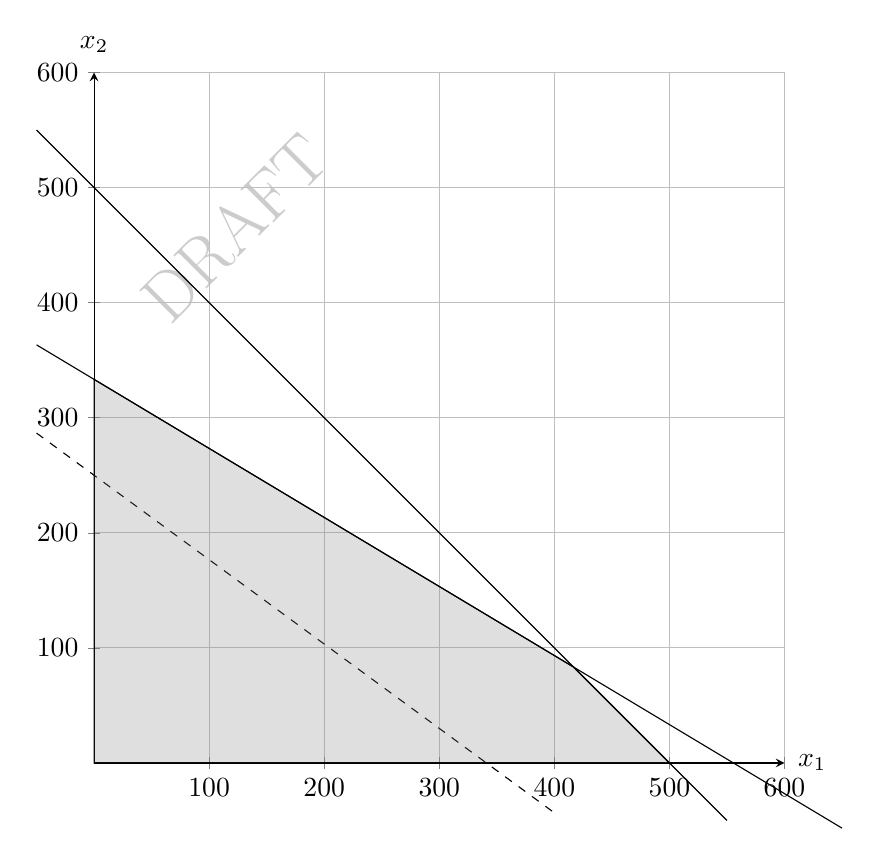
\begin{tikzpicture}
  \begin{axis}[ width=12cm,
    unit vector ratio*=1 1 1,
    enlargelimits=false,
    grid=both,
    axis x line=middle,
    axis y line=middle,
    title=,
    clip=false,
    ymin=0, ymax=600,
    xmin=0, xmax=600]

    \addplot[domain=-50:650] {50000/150 - 90/150*x};
    \addplot[domain=-50:550] {500 - x};
    \addplot[domain=-50:400,dashed] {250 - 110/150*x};
    \addplot[fill=gray, fill opacity=.25]
    coordinates { (0,0) (500,0) (416.67,83.33) (0,333.33) } \closedcycle;

  % to get axis labels at the end of the axis
  \node at (axis description cs:1.04,0) {$x_1$}; \node at
  (axis description cs:0,1.04) {$x_2$};
\end{axis}
\end{tikzpicture}
\end{center}
\caption{Feasible region for the farm problem.}
\label{fig:feasibleregion}
\end{figure}

We now show how to model the farm problem in GAMS.
The complete problem formulation is shown in
figure~\ref{fig:farmer}.

\begin{SaveVerbatim}{vrbfarmer}
variables
x1 'acres of feed corn'
x2 'acres of organic corn'
z;
positive variables x1, x2;

equations
 profit  'objective function'
 budget  'available cash'
 acres   'available acres';

profit.. z =e= 110*x1 + 150*x2;
budget.. 90*x1 + 150*x2 =l= 50000;
acres.. x1 + x2 =l= 500;

model farmer / all /;

solve farmer using LP maximizing z;
\end{SaveVerbatim}

\begin{figure}
\fbox{
\begin{minipage}{\textwidth}
\BUseVerbatim{vrbfarmer}
\caption{Farm problem (\texttt{farmer.gms})}
\label{fig:farmer}
\end{minipage}
}
\end{figure}


Since this problem is small, we include all data parameters directly
in the model specification. However, it is usually good practice to
separate the data from the model, and AMPL encourages this separation
by providing \texttt{param} declarations and the ability to have a
separate \texttt{data} section. We will illustrate these features of
AMPL in the other problem formulations in this article.  AMPL doesn't
actually solve the mathematical programing problem, but rather passes
a description of the problem to a solver, which returns information
about the solution (if any solution was found) to AMPL. An AMPL
session for the forestry problem follows:

\begin{Verbatim}[samepage=true]
ampl: model forester.mod;
ampl: solve;
MINOS 5.5: optimal solution found.
2 iterations, objective 6250
ampl: display x1,x2;
x1 = 25
x2 = 75
\end{Verbatim}

The optimal solution indicates that the forester should harvest 100
acres, but let 25 acres regenerate naturally and plant 75 acres with
pine, for a profit of \$6250. Notice that the entire budget of \$4000
is exhausted because $10 \times 25 + 50 \times 75 = 4000$. When a
resource capacity constraint such as \texttt{acres} or \texttt{budget}
holds with equality in the optimal solution (as in this example), then
the constraint is \emph{binding}; all of the resource associated with
the constraint is being consumed. If more/less of the resource were
available, then profit would be increased/decreased. The value of the
associated dual variable indicates the amount by which profit would be
affected for small changes in the supply of the resource. This is
called the marginal value of a resource, or the shadow price.

\begin{Verbatim}[samepage=true]
ampl: display acres, budget;
acres = 32.5
budget = 0.75
\end{Verbatim}

Displaying the shadow prices in AMPL indicates that an additional acre
of hardwood timber would increase profit by \$32.50, given the same
budget of \$4000.  Modifying the right-hand side of \texttt{acres} to
101 and re-solving shows that this is indeed the case.

\begin{Verbatim}[samepage=true]
ampl: reset;
ampl: model forester.mod;
ampl: expand acres;
subject to acres:
	x1 + x2 <= 101;

ampl: solve;
MINOS 5.5: optimal solution found.
2 iterations, objective 6282.5
ampl: display x1,x2;
x1 = 26.25
x2 = 74.75
\end{Verbatim}

The \texttt{expand} command displays the full form of a set of
constraints.  (This will be useful for indexed expressions.) Notice
that the values of the decision variables have necessarily changed and
that the solution is no longer integer-valued.  This is typical of
resource allocation problems. We are in fact assuming that the
forester is able to execute the decisions on partial acres.  For the
\texttt{budget} constraint, an additional one dollar increase/decrease
in the right-hand side would increase/decrease profit by \$0.75, given
the same 100 acres of hardwood. It stands to reason, then, that the
forester could take out a loan and apply the funds to her
operation. As long as the interest rate is less than .75, profit will
increase.

Shadow prices are valid for \emph{limited} increases/decreases in the
right-hand sides of the constraints. The ranges over which the these
values are valid is a topic of sensitivity analysis. Here, we will
show how to extract this information from AMPL. First we need to tell
AMPL to use a solver that is able to return sensitivity information
along with the optimal solution. We will use the solver
\texttt{cplex}. Then we set a solver-specific option to make the
sensitivity range information available.

\begin{Verbatim}[samepage=true]
ampl: option solver cplex;
ampl: option cplex_options 'sensitivity';
ampl: solve;
CPLEX 11.2.0: sensitivity
CPLEX 11.2.0: optimal solution; objective 6250
2 dual simplex iterations (1 in phase I)

suffix up OUT;
suffix down OUT;
suffix current OUT;
\end{Verbatim}

We are now able to display the ranges over which the current shadow
prices of \$32.5 per acre and \$0.75 per dollar of budget are
valid. To do this we simply add a suffix to the name of the
constraint, separated by a ``\texttt{.}''. The suffix
\texttt{.current} displays the current value of a constraint's
right-hand side, while \texttt{.down} and \texttt{.up} display the
lower and upper limits, respectively. In the AMPL session follows, the
upper limit of 5000 on the right-hand side of \texttt{budget}
indicates the forester should only consider loans of \$1000 or less to
be valued at an incremental marginal value of 0.75.

\begin{Verbatim}[samepage=true]
ampl: display acres.down, acres.current, acres.up;
acres.down = 80
acres.current = 100
acres.up = 400

ampl: display budget.down, budget.current, budget.up;
budget.down = 1000
budget.current = 4000
budget.up = 5000
\end{Verbatim}

Sensitivity ranges may also be obtained for the decision variables. In
this case the lower and upper limits represent the valid ranges on the
objective function coefficients over which the current solution
remains optimal.  The suffix \texttt{.current} refers to the current
value of the coefficient.  Displaying this information for the
forestry problem reveals that the current solution value of \texttt{x1
  = 25} remains optimal as long as its coefficient in the objective
function is in the range 14 to 70, holding all other parameters at
their current values.

\begin{Verbatim}[samepage=true]
ampl: display x1.down, x1.current, x1.up;
x1.down = 14
x1.current = 40
x1.up = 70

ampl: display x2.down, x2.current, x2.up;
x2.down = 40
x2.current = 70
x2.up = 200
\end{Verbatim}

\emph{A Diet Problem.}
Dwight is an elementary school teacher who also raises pigs for
supplemental income. He is trying to decide what to feed his pigs.
Considering a combination of pig feeds available from local suppliers,
he would like to feed the pigs at minimum cost while also making sure
each pig receives an adequate supply of calories and vitamins.  The
cost, calorie content, and vitamin content of each feed are given in
the table below.

\vspace{.1in}
\begin{center}
\begin{tabular}{ccc}
\textbf{Contents}   &  \textbf{Stark County Coop Pig Feed }   & \textbf{Pioneer Pig Feed} \\   \hline
Calories (per pound)  &  800    &  1000   \\
Vitamins (per pound)  &  140 units  &  70 units  \\
Cost (per pound)   &  \$0.40    & \$0.80  \\
\end{tabular}
\end{center}
\vspace{.1in}

Each pig requires at least 8,000 calories per day and at least 700
units of vitamins. A further constraint is that no more than one-third
of the diet (by weight) can consist of Stark County Coop Pig Feed,
since it contains an ingredient which is toxic if consumed in too
large a quantity.  First, let's write down the mathematical
programming formulation without regard to AMPL. Let $x_1$ be the
pounds per day of Stark County Coop feed to purchase. Similarly, let
$x_2$ be the pounds per day of Pioneer feed to purchase. Then the
problem is to 

\[
\begin{array}{lrrrrrl}
\textrm{minimize}   & .4x_1 & + & .8x_2 &  &  &  \\
\textrm{subject to} & 800x_1 & + & 1000x_2 & \geq & 8000 & \textrm{(calories)} \\
                    & 140x_1 & + & 70x_2   & \geq & 700  & \textrm{(vitamins)} \\
					& 2x_1   & - & x_2     & \leq & 0    & \textrm{(toxicity)} \\
\multicolumn{4}{r}{x_1,x_2}& \geq & 0 &
\end{array}.
\]

To get the toxicity restriction on the amount of Stark County Coop
feed, begin with the relation
\[
x_1 \leq \frac{1}{3}(x_1 + x_2).
\]
Then collect terms and simplify.  Since this problem has only two
variables, we can easily specify the model in AMPL by creating each
variable, the objective function, and the three constraints as shown
in Figure~\ref{p1}. This model should be saved in a text file with a
\texttt{.mod} extension.

\begin{SaveVerbatim}{pigs}
var x1 >= 0;  # stark
var x2 >= 0;  # pioneer

minimize total_cost: .4*x1 + .8*x2;

subject to cal: 800*x1 + 1000*x2 >= 8000;
subject to vit: 140*x1 + 70*x2 >= 700;
subject to tox: x1 <= (1/3)*(x1 + x2);
\end{SaveVerbatim}

\begin{figure}
\fbox{
\begin{minipage}{\textwidth}
\BUseVerbatim{pigs}
\caption{AMPL model (\texttt{pigs.mod})}
\label{p1}
\end{minipage}
}
\end{figure}

The following AMPL session shows how to read the problem into AMPL,
invoke the default solver, and print the solution. The minimum cost
feed mixture is 2.86 pounds of Stark County feed and 5.71 pounds of
Pioneer feed per pig per day, for a total cost of \$5.71 per pig per
day.
\begin{Verbatim}[samepage=true]
ampl: model pigs.mod;
ampl: solve;
MINOS 5.51: optimal solution found.
2 iterations, objective 5.714285714
ampl: display x1, x2;
x1 = 2.85714
x2 = 5.71429
\end{Verbatim}

For problems of any reasonable size it is necessary (and desirable) to separate
the model and data. This will allow us to solve different problem instances
(i.e. different sets of data) without changing the model. Figure~\ref{p2} shows
the complete problem formulation and data with separate \texttt{model} and
\texttt{data} sections in the same text file (\texttt{pigs2.mod}). It is also
possible (and you will usually want to do this) to put the data section
in its own text file. In that case we would name the data file with a
\texttt{.dat} extension, e.g. \texttt{pigs2.dat}.

\begin{SaveVerbatim}{pigs2}
model;
set Supplier;

param calories {Supplier};  # per pound
param vitamins {Supplier};  # units per pound
param cost {Supplier};      # dollars per pound

var x {Supplier} >= 0;  # pounds to purchase from each supplier (per pig)

minimize total_cost: sum {i in Supplier} cost[i]*x[i];

s.t. cal: sum {i in Supplier} calories[i]*x[i] >= 8000;
s.t. vit: sum {i in Supplier} vitamins[i]*x[i] >= 700;
s.t. tox: x['stark'] <= (1/3)* sum {i in Supplier} x[i];

data;
set Supplier := stark pioneer;

param : vitamins cost calories:=
stark   140      .4    800
pioneer  70      .8   1000;
\end{SaveVerbatim}

\begin{figure}
\fbox{
\begin{minipage}{\textwidth}
\BUseVerbatim{pigs2}
\caption{Separation of model and data (\texttt{pigs2.mod})}
\label{p2}
\end{minipage}
}
\end{figure}

Most AMPL models are specified by declaring sets, parameters, and
variables, and then by writing the objective function and the
constraints that make use of the sets, parameters, and
variables. Parameters are typically numeric values, although they can
also be logical or symbolic values. They can be thought of as ``data''
values, e.g. the cost per pound of feed. Variables represent the
decisions, e.g. the amount of feed to purchase. Sets specify the
objects with which parameters and variables are associated. We
declared the feed suppliers to be a set because the decisions for how
much feed to purchase as well as cost and nutritional attributes of
the feed are logically associated with each supplier. We say that the
parameters and the variables are \emph{indexed} over the set of
suppliers.

Giving short, meaningful names to sets, parameters, and variables
makes a model readable.  I like to capitalize the first letter of set
names so that they are easily distinguished from parameters.  In the
AMPL book, you will see that set names are in all upper-case
letters. This is just a convention, and the language does not require
it; however, good programming habits will make your code easier to
maintain.

Here is the output from an AMPL session using the model and data in
\texttt{pigs2.mod}.  When working with AMPL, if you read in a model
and subsequently make changes, or if you read in a new model after
having worked with an initial model, you will need to use the
\texttt{reset} command before reading in the new model. Note that when
the decision variables are indexed over a set, we display all of them
at once by typing the variable symbol.
\begin{Verbatim}[samepage=true]
ampl: reset;
ampl: include pigs2.mod;
ampl: solve;
MINOS 5.51: optimal solution found.
2 iterations, objective 5.714285714
ampl: display x;
x [*] :=
pioneer  5.71429
  stark  2.85714
;
\end{Verbatim}

\emph{Factory Planning.}
This example is taken from~\cite{williams:1999}. 
A factory makes seven products that require various amounts of time on four different
types of machines. The factory owns four grinders, two vertical drills, three 
horizontal drills, one boring machine, and one planing machine. 
For each product manufactured, the company can either sell the
product (subject to market limitations) or hold the product in inventory at a cost of
.5 per unit per month. We would like to develop a production and inventory plan for
each of the next six months.
We will not consider the sequence of machine operations; however, there
is a fixed maintenance schedule that specifies when and how many of each machine type
will be unavailable. The factory operates two eight-hour shifts each working day.
There are 24 working days each month.

Refer to the data in figure~\ref{fdat} as well as the model in
figure~\ref{fmod} while reading this description.
Notice that the set \texttt{Month} is declared to be of type \texttt{ordered},
indicating a defined ordering among its (symbolic) members.
This means that we can refer to the members of \texttt{Month} by their relative position.
For example, in our data the expression \texttt{first(Month)} refers
to the member \texttt{'jan'}. One common reason for declaring a set to be \texttt{ordered}
is the need to refer to the previous and/or the next member in an indexed expression.
A typical example of this use of an \texttt{ordered} set is illustrated by the 
\texttt{balance} constraints.

\begin{SaveVerbatim}{vrbfmod}
set Product;
set Machine;
set Month ordered;

param profit {Product} >= 0;
param time_required {Product,Machine} >= 0;
param num_available {Machine} integer, >= 0;
param downtime {Month,Machine} integer, >=0;
param market_limit {Month,Product} integer, >= 0;
param work_hours := 2*8*24;
# number of working hours in a month: 2 shifts of 8 hours each, 24 days/month

var make {Month,Product} >=0;  # how much of each product to make in each month
var sell {Month,Product} >=0;  # how much to sell
var hold {Month,Product} >=0, <=100;  # how much to hold

maximize total_profit:
  sum {t in Month, i in Product} (profit[i]*sell[t,i] - 0.5*hold[t,i]);

s.t. capacity {t in Month, m in Machine}:
sum {i in Product} time_required[i,m]*make[t,i] 
  <= work_hours*(num_available[m]-downtime[t,m]);

s.t. marketing {t in Month, i in Product}: sell[t,i] <= market_limit[t,i];

s.t. balance {t in Month, i in Product : ord(t) > 1}:
  hold[prev(t),i] + make[t,i] = sell[t,i] + hold[t,i];
# on-hand inventory plus number produced must equal number
# sold plus number held in inventory for the next period

s.t. balance0 {i in Product}:
  make[first(Month),i] = sell[first(Month),i] + hold[first(Month),i];
# there is no inventory held over from december

s.t. end_inventory {i in Product}: hold[last(Month),i] = 50;
# stipulate that 50 of each product are to be held over from june
\end{SaveVerbatim}

\begin{figure}
\fbox{
\begin{minipage}{\textwidth}
\BUseVerbatim{vrbfmod}
\caption{Model for factory planning problem (\texttt{factory\_planning1.mod})}
\label{fmod}
\end{minipage}
}
\end{figure}

A defining feature of this model is use of three different variables to represent
the quantities and timing for making, selling, and holding each product.
The relationship among these
variables is stated in the \texttt{balance} constraints.
An upper bound of 100 units on the \texttt{hold} variable represents a storage limitation 
for each product in each month.

Our objective is to maximize the total profit of the factory over a period of six months.
A unit profit is accrued for each item sold and a unit cost of .5 is incurred for each item
held in inventory in a given month.
Note that the parentheses surrounding the subtraction
are necessary because the \texttt{sum} operator has higher precedence than \texttt{-}.
As a side note, if we were to remove the holding cost from consideration in 
the objective then no parentheses would be required around the
\texttt{profit[i]*sell[t,i]} term because the \texttt{sum} operator has lower precedence
than \texttt{*}~\cite{fourer:2003}. 

Each product requires a certain amount of processing time (possibly zero) on each type
of machine. These requirements are specified in the data by the parameter 
\texttt{time\_required} that is indexed over \texttt{Product} and \texttt{Machine}
We need to specify constraints on the amount of machine time
available each month. There are \texttt{work\_hours} production hours available each month
on each machine unless a machine is down for maintenance. Because the maintenance
schedule is specific to each machine and month, the machine capacity constraints 
are indexed over \texttt{Month} and \texttt{Machine}. The total number of machine
hours for all products must not exceed the time available in any particular month
(respecting the \texttt{downtime} schedule.)
There is an upper bound on the amount of each product that the market will absorb
(i.e. that can be sold) each month.

We have three different variables to represent the decisions to make, sell,
and hold product.  The logical relationship among these variables is that
in any particular month the amount sold plus the amount held in inventory
must equal the amount produced plus any inventory from the previous month.
When specifying these product balance constraints we must pay attention to the
boundary conditions when indexing over \texttt{Month}. In our problem, we
cannot refer to the previous month when the dummy index evaluates to \texttt{'jan'}.
We can handle this in the main \texttt{balance} equations by placing a condition
on the indexed set such that the order of the member is greater than 1
(and so \texttt{'jan'} is omitted.)
This is possible because we declared the set \texttt{Month} to be of type
\texttt{ordered}. We then need to specify a separate set of constraints for
the first month (\texttt{balance0}). There is no beginning inventory and 
so the amount produced in \texttt{'jan'} equals the amount sold plus the amount
held.

Instead of using the expression \texttt{make[first(Month),i]},
it would have been legitimate to refer to \texttt{make['jan',i]}; however,
it's better practice to separate the model from the data. The model may then
be applied to other problem instances with the same structure, but perhaps with
a different starting month. Finally, we would like to end June with 50 of
each product type in inventory. This is specified by the equality constraints
named \texttt{end\_inventory}.

\begin{SaveVerbatim}{vrbfdata}
data;
set Product := 1 2 3 4 5 6 7;
set Machine := grinder vdrill hdrill borer planer;
set Month := jan feb mar apr may jun;

param profit := 1 10 2 6 3 8 4 4 5 11 6 9 7 3;

param num_available :=	
grinder 4 vdrill 2 hdrill 3 borer 1 planer 1;

param time_required (tr) :
         1   2   3   4   5   6   7 :=
grinder .5  .7   0   0  .3  .2  .5
vdrill  .1  .2   0  .3   0  .6   0
hdrill  .2   0  .8   0   0   0  .6
borer  .05 .03   0 .07  .1   0 .08
planer   0   0 .01   0 .05   0 .05;

param downtime :
     grinder vdrill hdrill borer planer :=
jan    1       0     0      0     0
feb    0       0     2      0     0
mar    0       0     0      1     0
apr    0       1     0      0     0
may    1       1     0      0     0
jun    0       0     1      0     1;

param market_limit :
       1     2     3     4     5     6     7 :=
jan  500  1000   300   300   800   200   100
feb  600   500   200     0   400   300   150
mar  300   600     0     0   500   400   100
apr  200   300   400   500   200     0   100
may    0   100   500   100  1000   300     0
jun  500   500   100   300  1100   500    60;
\end{SaveVerbatim}

\begin{figure}
\fbox{
\begin{minipage}{\textwidth}
\BUseVerbatim{vrbfdata}
\caption{Data for factory planning problem (\texttt{factory\_planning1.mod})}
\label{fdat}
\end{minipage}
}
\end{figure}

\section{Integer Programming}

\emph{Perfect Matching.}
There are 10 students to be assigned to 5 dorm rooms. Each room holds exactly
two students. For each pair of students, a value that indicates the desirability
of placing that pair in the same room has been determined. Higher values 
correspond to better pairings.
We would like to pair the students in such a way that the
sum total of the values of each assigned pair is maximized. More generally,
the perfect matching problem is to assign $n$ pairs for $2n$ objects (with or without
an objective function). The model and data are presented in figure~\ref{perfect}.

\begin{SaveVerbatim}{vrbperfect}
set Student; 
set Pair within Student cross Student;

param value {Pair};

var x {Pair} binary;

maximize total_value: sum {(i,j) in Pair} value[i,j] * x[i,j];

s.t. perfect_match {i in Student}:
	sum {(i,j) in Pair} x[i,j] + sum {(j,i) in Pair} x[j,i] = 1;

data;
set Student := 1 2 3 4 5 6 7 8 9 10;

param: Pair: value:
   1  2  3  4  5  6  7  8  9 10 :=
1  .  .  .  .  .  .  .  .  .  .
2  3  .  .  .  .  .  .  .  .  .
3  5  8  .  .  .  .  .  .  .  .
4  1 -4  7  .  .  .  .  .  .  .
5  2 -1  9  2  .  .  .  .  .  .
6  2  5  3  2  9  .  .  .  .  .
7  8  2  1  1  3 -2  .  .  .  .
8  2  3  3  4  5  1  1  .  .  .
9 13 -1  3  4  4 -5  2  2  .  .
10 1  2  6  6  7 -4  5  6  1  .;
\end{SaveVerbatim}

\begin{figure}
\fbox{
\begin{minipage}{\textwidth}
\BUseVerbatim{vrbperfect}
\caption{Model and data for perfect matching problem (\texttt{roommates.mod})}
\label{perfect}
\end{minipage}
}
\end{figure}

\texttt{Pair} is a compound set with dimension two. Each member of this set is
an ordered pair of students. We use the term ``ordered'' because the member
(3,7) is distinct from the member (7,3). The \texttt{within} phrase tells
us that the only allowed members in \texttt{Pair} are ordered pairs from the set
\texttt{Student}. Such restrictions in the declaration of sets are encouraged in order to
help detect errors in the data. For example, the following alternative declaration is 
perfectly acceptable, but using it would not allow the AMPL translator to recognize
invalid pairs of students in the data section.
\begin{Verbatim}
set Pair dimen 2;
\end{Verbatim}

The declaration of \texttt{Pair} is not strictly necessary. We could formulate the problem
using only the set \texttt{Student}. However, using the compound set \texttt{Pair}
makes the model easier to read and to maintain, particularly the indexing expressions.
We specify a parameter \texttt{value} that is indexed over \texttt{Pair} to represent the
desirability of matching up a particular pair of students. Our decision variables
\texttt{x} are binary variables that are also indexed over \texttt{Pair}. 
\texttt{x[i,j]} will equal one if student \texttt{i} is matched with student \texttt{j},
and will equal zero otherwise. Notice the \texttt{binary} modifier in the declaration
of \texttt{x}. This means that our decision variables may \emph{only} take on the values zero
or one and turns our formulation into one of pure integer programming~\cite{nemhauser:1988}.

The problem formulation itself consists of the objective function and a single set
of constraints, one for each student. Our objective is to maximize the overall
value of the assignments. It provides a good example of how to iterate over a 
compound set in AMPL. Notice that we must provide a pair of dummy variables
\texttt{(i,j)} to index into \texttt{Pair}. 

The constraints \texttt{perfect\_match} state that each student must be
matched with exactly one other student. To understand how this is 
accomplished note that the scope of the index \texttt{i} extends from 
its introduction in \texttt{i in Student} until the end of the statement
marked by the semi-colon. In the expression \texttt{sum \{(i,j) in Pair\} x[i,j]},
\texttt{i} is held constant for a particular student (row of \texttt{value}) 
and the summation is over all room mates such that the pair of students
represented by \texttt{(i,j)} exist in the set \texttt{Pair}, i.e. the
summation is over columns.
In the second expression with \texttt{i} and \texttt{j} interchanged, the
summation is over rows. This is necessary
due to the way that the data for \texttt{Pair} are structured. Notice that
only the lower left portion of \texttt{value} is filled in.

This example demonstrates how to simultaneously define a set (\texttt{Pair}) and a parameter
(\texttt{value}) that is indexed over that set. The ``\texttt{.}'' symbols indicate
missing values, e.g. there exists no member \texttt{(1,1)} in the set \texttt{Pair}.
An AMPL session for solving this problem follows. Although not strictly necessary
for this particular problem, we will instruct AMPL to use
a solver that can handle integer programming problems, such as the solver
\texttt{gurobi}. 

\begin{Verbatim}[samepage=true]
ampl: option solver gurobi;
ampl: model roommates.mod;
ampl: solve;
Gurobi 3.0.0: optimal solution; objective 39
14 simplex iterations
ampl: display x;
x [*,*]
:    1   2   3   4   5   6   7   8   9    :=
2    0   .   .   .   .   .   .   .   .
3    0   1   .   .   .   .   .   .   .
4    0   0   0   .   .   .   .   .   .
5    0   0   0   0   .   .   .   .   .
6    0   0   0   0   1   .   .   .   .
7    0   0   0   0   0   0   .   .   .
8    0   0   0   1   0   0   0   .   .
9    1   0   0   0   0   0   0   0   .
10   0   0   0   0   0   0   1   0   0
;
\end{Verbatim}

The large number of zeros makes the solution difficult to read. A useful
option is to only display the decision variables with nonzero values. Then
we can easily see that the pairs are (3,2),(6,5),(8,4),(9,1), and (10,7).

\begin{Verbatim}[samepage=true]
ampl: option omit_zero_rows 1;
ampl: display x;
x :=
3  2   1
6  5   1
8  4   1
9  1   1
10 7   1
;
\end{Verbatim}

\emph{Map Coloring.}
The map coloring problem is to assign a color to each area on a map
(e.g. state or county) in such a way that adjacent areas (i.e. those
areas that share a border) are assigned different colors. Moreover, we 
would like to use as few colors as possible. The formulation for this
problem was adapted from code written in GNU MathProg by Andrew
Makhorin~\cite{glpk}.

We may create a representation of the adjacency information by constructing a
graph wherein each area on the map is represented by a node. An 
edge is drawn between two nodes if the respective areas on the map share a border.
As an example, figure ? shows the map and the corresponding
adjacency graph for the western United States. The graph representation
will better facilitate the requirement that adjacent areas must be assigned 
different colors.

\begin{figure}
\begin{center}
\includegraphics[scale=0.7]{westernusa.pdf}
\caption{Western states and adjacency graph}
\label{westernusa}
\end{center}
\end{figure}

Both the model and the data are presented in figure~\ref{kcolor}. In this model
we must make the cardinality of the set \texttt{Color} large enough to effect
a feasible solution. For a large problem the minimum number of colors needed will not
be obvious (otherwise there is no need to solve the problem.) However, if the 
solver finds that the problem is infeasible we can always add more members to the
set \texttt{Color}. See Andrew Makhorin's code~\cite{glpk} for an implementation
of a heuristic to obtain an upper bound on the required number of colors.

\begin{SaveVerbatim}{vrbkcolor}
set Node;
set Edge within (Node cross Node);
set Color;   
# the cardinality of the set Color needs to be large enough
# to find a feasible solution

var x {Node,Color} binary; # x[i,c] = 1 means that node i is assigned color c
var u {Color} binary;      # u[c] = 1 means that color c is used

minimize num_colors: sum {c in Color} u[c];

s.t. assignment {i in Node}: sum {c in Color} x[i,c] = 1;
# each node is assigned exactly one color

s.t. different {(i,j) in Edge, c in Color}: x[i,c] + x[j,c] <= u[c];
# adjacent nodes must be assigned different colors

data;
set Color := red blue green yellow orange;

set Node := ca or wa mt id nv wy ut az;

set Edge:
   ca or wa mt id nv wy ut az :=
ca -  +  -  -  -  +  -  -  +
or -  -  +  -  +  +  -  -  -
wa -  -  -  -  +  -  -  -  -
mt -  -  -  -  +  -  +  -  -
id -  -  -  -  -  +  +  +  -
nv -  -  -  -  -  -  -  +  +
wy -  -  -  -  -  -  -  +  -
ut -  -  -  -  -  -  -  -  +
az -  -  -  -  -  -  -  -  -;
\end{SaveVerbatim}

\begin{figure}
\fbox{
\begin{minipage}{\textwidth}
\BUseVerbatim{vrbkcolor}
\caption{Model and data for map coloring problem (\texttt{kcolor.mod})}
\label{kcolor}
\end{minipage}
}
\end{figure}

Our binary decision variables \texttt{x} will indicate the particular color 
assigned to each node (area on the map). We also create binary modeling variables
\texttt{u} to indicate that a color has been used in the solution. Now the
objective is a simple summation over \texttt{u}. There are three dummy variables
in the indexing expression for the \texttt{different} constraint. Notice
that even though \texttt{x} is indexed over \texttt{\{Node,Color\}} the
indexing expression for \texttt{different} will only create one constraint for
each existing \texttt{Edge} and \texttt{Color} combination. Since \texttt{Edge}
is declared to be \texttt{within (Node cross Node)} we may safely use the
dummy indices \texttt{i} and \texttt{j} when indexing into \texttt{x}.

In the \texttt{data} section we see one way to specify the members of a 
two-dimensional set: the ``\texttt{+}'' symbols indicate membership while the
``\texttt{-}'' symbols indicate non-membership. Alternatively, we could have
specified \texttt{Edge} by providing only the ordered pairs.
\begin{Verbatim}[samepage=true]
set Edge :=
(ca,or)   (ca,az)   (or,id)   (wa,id)   (mt,wy)   (id,wy)   (nv,ut)   (wy,ut)
(ca,nv)   (or,wa)   (or,nv)   (mt,id)   (id,nv)   (id,ut)   (nv,az)   (ut,az);
\end{Verbatim}

\section{Deterministic Dynamic Programming}

\section{Deterministic Inventory Models}

\clearpage
\section{Exercises}
\begin{enumerate}

\subsubsection*{Linear Programming}

% written by Hannah
\item \emph{Feasible region for an LP.} Indicate graphically whether each of the following
  linear programs has a feasible solution. Graphically determine the
  optimal solution, if one exists, or show that no optimal solution
  exists.

\begin{enumerate}
\item
\[
  \begin{array}{lrrrrr}
    \textrm{maximize}   & x_1& +& 3x_2&  & \\
    \textrm{subject to} & x_1& -&4x_2& \leq & 4  \\
                        & x_1& +& 2x_2& \leq & 4 \\
    \multicolumn{3}{r}{x_1,x_2}&       \geq & 0 
  \end{array}
\]

\item
\[
  \begin{array}{lrrrrr}
    \textrm{minimize}   & x_1& +& 2x_2&  & \\
    \textrm{subject to} & 2x_1& -&x_2& \leq & 3  \\
                        & 2x_1& -& x_2& \geq & -3 \\
    \multicolumn{3}{r}{x_1,x_2}&       \geq & 0 
  \end{array}
\]

\end{enumerate}

\begin{solution}
\bs The feasible region for the linear program in part a) is shown
below. The objective function is plotted as a dashed line. The
optimal solution occurs at $x_1=0$, $x_2=2$, and value of the
objective function at the optimal solution is $z=6$.

\begin{center}
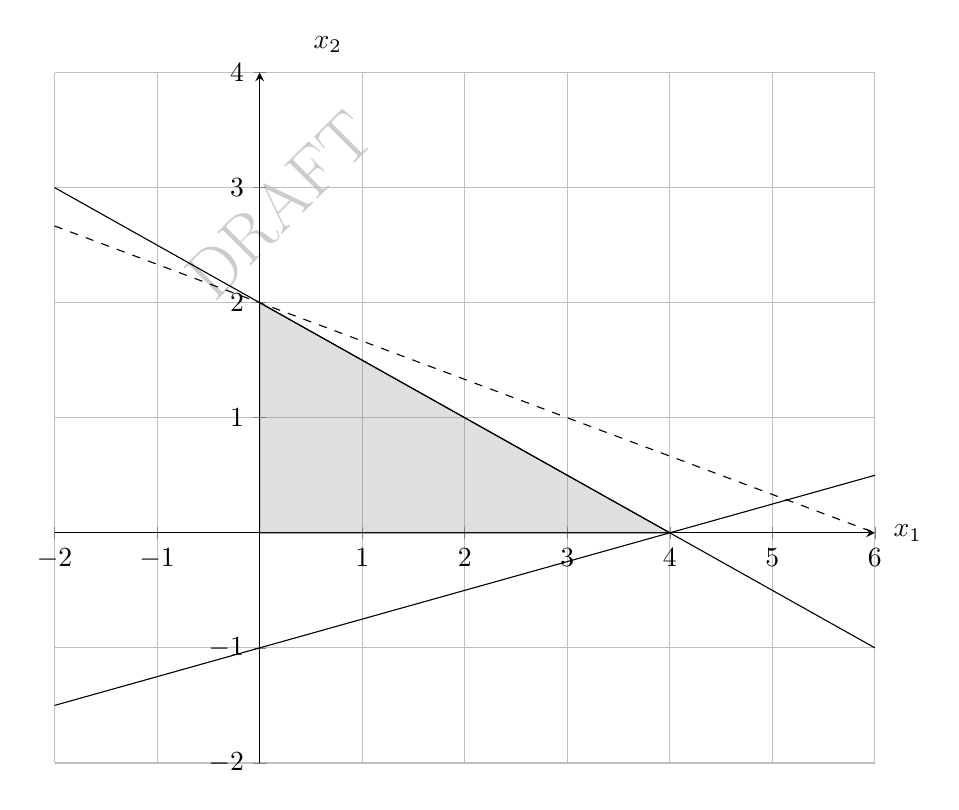
\begin{tikzpicture}
  \begin{axis}[ width=12cm, grid=both, axis x line=middle, axis y
    line=middle, title=, clip=false, ymin=-2, ymax=4, xmin=-2,
    xmax=6 ]

    \addplot[domain=-2:6] {-1 + 1/4*x}; \addplot[domain=-2:6] {2
      - 1/2*x}; \addplot[domain=-2:6,dashed] {2 - 1/3*x};
    \addplot[fill=gray, fill opacity=.25] coordinates { (0,0)
      (4,0) (0,2) }\closedcycle;

    % to get axis labels at the end of the axis
    \node at (axis description cs:1.04,.333) {$x_1$}; \node at
    (axis description cs:.333,1.04) {$x_2$};
  \end{axis}
\end{tikzpicture}
\end{center}

The feasible region for the linear program in part b) is unbounded;
however, since it is a minimization problem, it has an optimal
solution at $x_1=0$, $x_2=0$. The value of the objective function at
the optimal solution is $z=0$.

\begin{center}
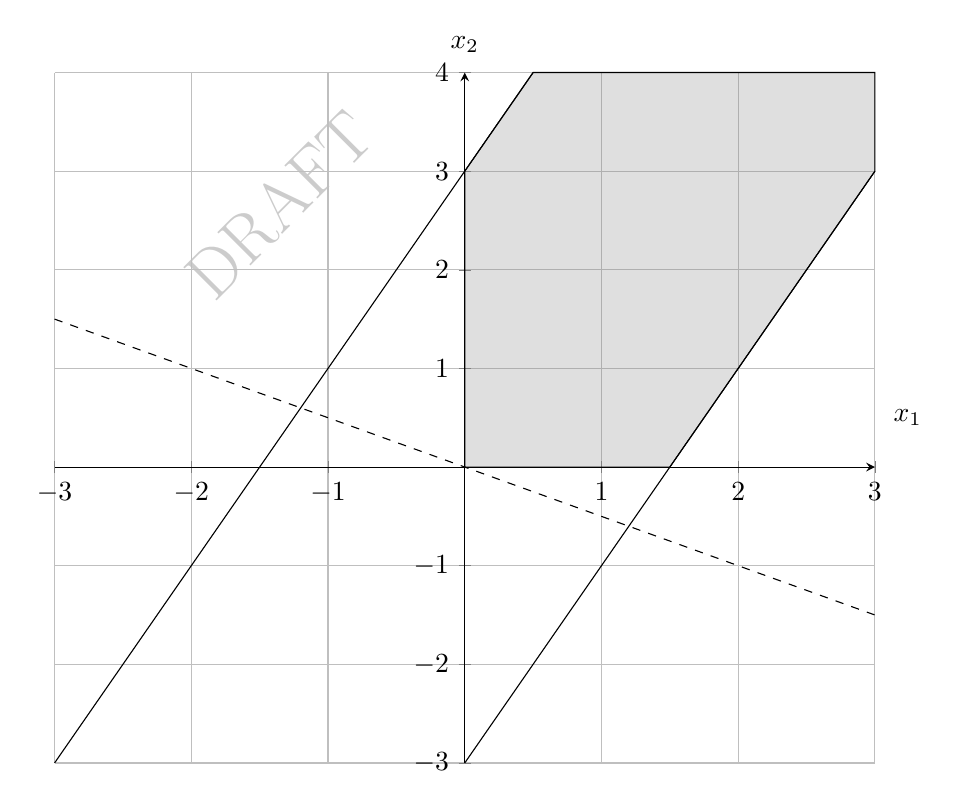
\begin{tikzpicture}
  \begin{axis}[ width=12cm, grid=both, axis x line=middle, axis y
    line=middle, title=, clip=false, ymin=-3, ymax=4, xmin=-3,
    xmax=3 ]

    \addplot[domain=0:3] {-3 +2*x}; \addplot[domain=-3:.5] {3+2*x};
    \addplot[domain=-3:3,dashed] {-1/2*x}; \addplot[fill=gray, fill
    opacity=.25] coordinates { (0,0) (0,3) (.5,4) (3,4) (3,3) (1.5,0)
    }\closedcycle;

    % to get axis labels at the end of the axis
    \node at (axis description cs:1.04,.5) {$x_1$}; \node at (axis
    description cs:.5,1.04) {$x_2$};
  \end{axis}
\end{tikzpicture}
\end{center}

\end{solution}

% re-written by Hannah
\item \emph{Karl's garden.}
Karl is a local gardener who grows lettuce, broccoli, and carrots. His garden is 
400 ft$^2$, and each individual plant of lettuce, broccoli, and carrots occupies 
0.5 ft$^2$, 1.2 ft$^2$, and 0.25 ft$^2$, respectively. Karl recently learned that 
many of his neighbors are interested in purchasing his vegetables. After polling the 
neighborhood, he learned that he has demand for 350 lettuce plants, 350 broccoli plants, 
and 250 carrot plants. Karl estimates that he will earn a profit of \$9.50 per 
lettuce plant, \$12.80 per broccoli plant, and \$8.25 per carrot plant. How many 
plants of each type of vegetable should Karl grow to maximize profit? Solve this 
problem using optimization software.

\begin{solution}
  \bs A GAMS model is provided in the file
  \texttt{karls-garden.gms}. The solution indicates that Karl should
  grow 350 lettuce plants, 135 broccoli plants, and 250 carrot plants
  for a total profit of about \$\num{7120}. Note that we are ignoring
  any fractional values of the decision variables.
\end{solution}


% this problem needs to be re-written, but I think we can just
% change the context and leave the numbers as they are (or very close
% anyway). the idea is to extract a shadow price and use it
% to answer questions.
\item \emph{Workplace safety.}  A manufacturing
  company has assembled a safety committee to reduce the number of
  injuries sustained by employees at work. The company has allotted
  the committee a budget of \$100 each week for purchasing items that
  will increase employee safety. After analyzing past incidents, the
  safety committee has concluded that the most common work hazard is
  exposure to loud noises. As a result, the committee would like to
  purchase (i) earplugs and (ii) other PPE (personal protection
  equipment). The relative value (utility) of the safety items was
  investigated, and it was determined that earplugs provide 1.2 units
  of value for each dollar spent on other types of PPE. The safety
  committee would like to determine how to spend the budget to
  maximize the safety of employees, but the company does not want to
  spend more than \$70 on earplugs and \$50 on other PPE each
  week. The committee also has the option to save part of the money.
  Additionally, the company would like to know:
\begin{enumerate}
\item How the total value of its expenditures for safety would change
  if there were only \$99 to spend. \label{safetya}
\item How the total value would change if \$75 could be spent on
  earplugs.\label{safetyb}
\item Whether it would save any money if each dollar of savings would
  provide 1.1 units of value for each dollar spent on other
  PPE.\label{safetyc}
\end{enumerate}
Formulate the safety committee's spending decision as a linear program. Sketch
the feasible region and determine the optimal solution using the
graphical method.  Then solve the linear program using optimization
software and obtain post-optimality output (i.e. a sensitivity
report).  Use this output to answer each of the questions \ref{safetya},
\ref{safetyb}, \ref{safetyc}.

\begin{solution}
\bs In the problem formulation to maximize total value, let
\[
  \begin{array}{lcl}
    x_1 &=& \textrm{\$ to spend on earplugs} \\
    x_2 &=& \textrm{\$ to spend on other PPE}
  \end{array}
\]
Then the committee wants to solve the following problem.
\[
\begin{array}{lrrrrr}
\textrm{maximize}   & 1.2x_1& +& x_2&      &   \\
\textrm{subject to} & x_1& +&x_2& \leq & 100 \\
                    & x_1& & & \leq & 70 \\
                    & & & x_2& \leq & 50 \\
\multicolumn{4}{r}{x_1,x_2}&       \geq & 0
\end{array}
\]

The feasible region is given below. The optimal solution is $x_1=70$ and $x_2=30$
for a total value of 114.
\begin{center}
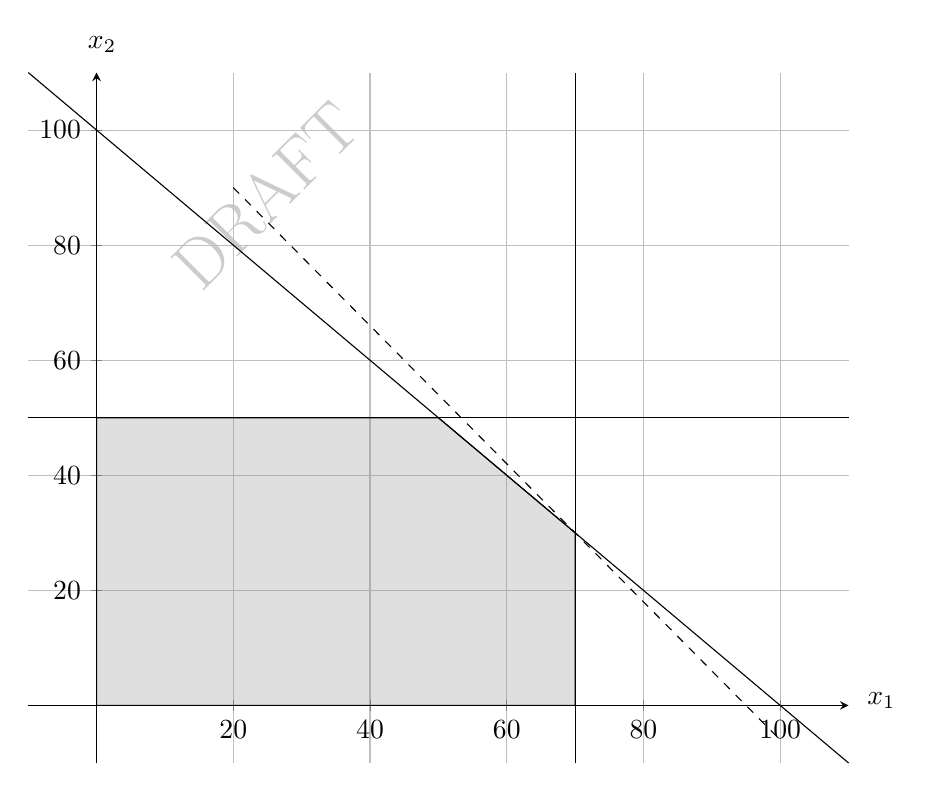
\begin{tikzpicture}
  \begin{axis}[ width=12cm, grid=both,
    axis x line=middle,
    axis y line=middle,
    title=, clip=false,
    ymin=-10, ymax=110, xmin=-10, xmax=110 ]

    \addplot[domain=-10:110] {-x + 100};
    \addplot[mark=none] coordinates {(70,-10) (70,110)};
    \addplot[domain=-10:110] {50};
    \addplot[fill=gray, fill opacity=.25] coordinates {
      (0,0) (70,0) (70,30) (50,50) (0,50) }\closedcycle;
    \addplot[domain=20:100,dashed] {-1.2*x + 114};

    % to get axis labels at the end of the axis
    \node at (axis description cs:1.04,.09) {$x_1$};
    \node at (axis description cs:.09,1.04) {$x_2$};
  \end{axis}
\end{tikzpicture}
\end{center}

A GAMS model is provided in \texttt{workplace-saftey.gms}. Refer to
the listing file \texttt{workplace-saftey.lst}, to answer questions
\ref{safetya}, \ref{safetyb}, and \ref{safetyc}.  Regarding part
\ref{safetya}, the shadow price on the \texttt{budget} constraint
tells us that if we decrease the RHS from 100 to 99, the value of the
objective function will decrease to 113. Since earplugs provide more
value than other PPE, the new solution will be $x_1=70$ and $x_2=29$.
For part \ref{safetyb}, notice that \$75 is within the range for the
shadow price on the \texttt{earplugs} constraint. So, increasing the
RHS to 75 will increase the total value by
\[ \$5 \times 0.2~\text{units of value per dollar} = 1 \]
for a total value of 115.
Finally, for part \ref{safetyc}, saving one dollar requires \$1; however, the
company gets 1.1 units of value for each dollar saved. Yes, the
company would save \emph{some} amount of money and spend less on other
PPE. To use the shadow price to answer this question, notice that the
shadow price on the \texttt{budget} constraint is 1. If we
``price-out'' the new activity of saving money, we see that it cost
\$1 per unit, but it returns \$1.1 per unit in total value. So the
company would save some amount of money. The question did not ask us
to determine the new solution. It only asked whether \emph{any} money
would be allocated to savings.
\end{solution}

% re-written by hannah
\item \emph{A blending problem.}  A pet food manufacturer is
  developing a new dog food recipe with natural ingredients. It has
  been decided that the recipe will contain a combination of 4
  ingredients: chicken, brown rice, vegetables, and corn meal. The
  cost and important nutritional information for each ingredient is
  summarized in the table below.

\begin{center}
\begin{tabular}{lcccc} \\
Ingredient  &   Cost (\$/lb)  & Protein (g/lb)  &  Fat (g/lb) &  Fiber (g/lb)  \\ \hline
(1) Chicken   &  3.00 & 125 & 60 & 0 \\
(2) Brown rice   &  0.75 & 12 & 4 & 9 \\
(3) Vegetables   &  1.80 & 14 & 1.5 & 12 \\
(4) Corn meal& 0.60 & 32 & 8 & 17
\end{tabular}
\end{center}

Industrial engineers have been asked to determine the most
cost-effective mixture of ingredients given the following guidelines:
\begin{compactitem}
\item Each pound of dog food must contain no more than 40 grams of fat.
\item Each pound of dog food must contain at least 80 grams of protein.
\item Each pound of dog food must contain at least 4 grams and no more
  than 10 grams of fiber.
\item Each ingredient must comprise at least 10\% of the mixture.
\end{compactitem}

\begin{enumerate}
\item Formulate an (algebraic) mathematical programming model using
  the information above and generate a solution using AMPL.  Your
  problem formulation can be a model for the minimum-cost way to
  produce one pound of dog food. We can consider that to be the
  ``recipe'' that would then be scaled up for production purposes.
  \label{doga}

\item Formulate an alternative (algebraic) mathematical programming
  model given the additional constraint that 80\% of the mixture must
  contain a combination of chicken and vegetables. Generate a solution
  using AMPL and determine the added cost due to the new
  constraint. \label{dogb}
\end{enumerate}

\begin{solution}
  \bs For part \ref{doga}, an AMPL model is provided in the file
  \texttt{dog-fooda.mod}.  The mixture should contain 55.7\% chicken,
  10\% brown rice, 10\% vegetables, and 24.3\% corn meal for a cost of
  \$2.07 per pound.
	
  For part \ref{dogb}, An AMPL model is provided in
  \texttt{dog-foodb.mod}. The added cost due to the additional
  constraint is \$0.20. The mixture should contain 58\% chicken, 10\%
  brown rice, 22\% vegetables, and 10\% corn meal for a cost of \$2.27
  per pound.
\end{solution}

% re-written by hannah
\item \emph{Maximum flow through a network.}  An industrial engineer
  is analyzing the drainage system at a food processing plant. The
  arrows in the following network indicate the direction of flow in
  the system, and the numbers indicate the capacity of each
  pipe. Formulate a linear programming problem to determine the
  maximum flow from source node $s$ to sink node $t$.

\vspace{.2in}
\begin{center}
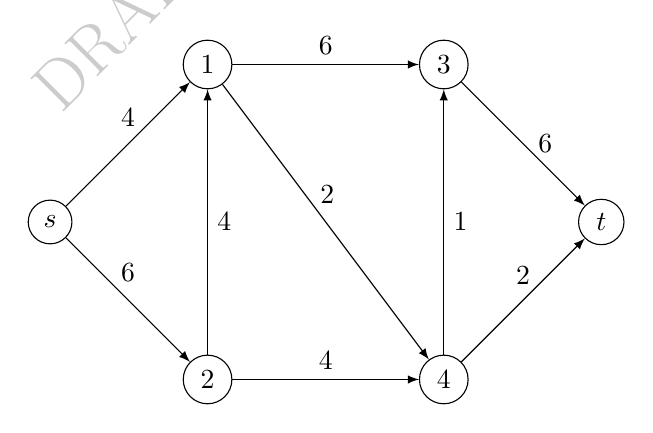
\begin{tikzpicture}[>=latex]

\node[circle,draw] (source) at (0,2) {$s$};
\node[circle,draw] (1) at (2,4) {1};
\node[circle,draw] (2) at (2,0) {2};
\node[circle,draw] (3) at (5,4) {3};
\node[circle,draw] (4) at (5,0) {4};
\node[circle,draw] (sink) at (7,2) {$t$};

\draw[->] (source) -- (1) node[above=3pt,pos=.5]{4};
\draw[->] (source) -- (2) node[above=3pt,pos=.5]{6};
\draw[->] (2) -- (1) node[right,pos=.5]{4};
\draw[->] (1) -- (3) node[above,pos=.5]{6};
\draw[->] (1) -- (4) node[right=2pt,pos=.4]{2};
\draw[->] (2) -- (4) node[above,pos=.5]{4};
\draw[->] (3) -- (sink) node[right=2pt,pos=.5]{6};
\draw[->] (4) -- (sink) node[above=2pt,pos=.5]{2};
\draw[->] (4) -- (3) node[right,pos=.5]{1};

\end{tikzpicture}
\end{center}

\begin{solution}
\bs
Add an artificial edge from sink node $t$ to source node $s$ that
has unlimited capacity. Let $x_{ij}$ be the amount of flow from node
$i$ to node $j$ for each directed edge $i,j$ that exists in the network.
The problem formulation is

\[
\begin{array}{lrrrrrrrrl}
\textrm{maximize}   & x_{ts} & & & & & & & \\
\textrm{subject to} & & & x_{s1} & + & x_{s2} & - & x_{ts} & = & 0 \\
& x_{13}&+ & x_{14} & - & x_{s1} & - & x_{21} & = & 0 \\
& & & x_{24} & + & x_{21} & - & x_{s2} & = & 0 \\
& & & x_{3t} & - & x_{13} & - & x_{43} & = & 0 \\
& x_{43} & + & x_{4t} & - & x_{14} & - & x_{24} & = & 0 \\
& & & x_{ts} & - & x_{3t} & - & x_{4t} & = & 0 \\
&&&&&&& x_{s1} & \leq & 4 \\
&&&&&&& x_{s2} & \leq & 6 \\
&&&&&&& x_{13} & \leq & 6 \\
&&&&&&& x_{21} & \leq & 4 \\
&&&&&&& x_{14} & \leq & 2 \\
&&&&&&& x_{24} & \leq & 4 \\
&&&&&&& x_{43} & \leq & 1 \\
&&&&&&& x_{4t} & \leq & 2 \\
&&&&&&& x_{3t} & \leq & 6 \\
\multicolumn{7}{r}{x_{ij}}&\geq & 0 & \text{for all edges $i,j$}
\end{array}
\]

\end{solution}

% re-written by Hannah
\item \emph{Golf lessons.}  Amy and Brian are professional
  golfers who have each agreed to donate 10 hours of private golf
  lessons to a charity auction. Three people have bid on the lessons,
  and their bids are shown in the table below. For example, Emma has
  bid \$28 per hour to receive lessons from Amy.

\begin{tabular}{lrr}
Bidder & Amy & Brian \\ \hline
Emma & \$28/hr & \$30/hr \\
Dan     & \$26/hr & \$28/hr \\
Sam  & \$30/hr & \$32/hr
\end{tabular}

In the spirit of fairness, the auction committee has decided that no bidder can win 
more than 8 hours of total instruction. Given the bid amounts, the committee must now
decide how to allocate the 20 hours of available instruction time.
\begin{compactenum}
  \item Draw a diagram of the problem as a network flow model.
  \item Formulate a linear programming model to maximize the
    charity's revenue.
  \item Solve the problem using optimization software.
\end{compactenum}

\begin{solution}
  \bs A diagram of the network flow model is shown below. Bidders 1, 2,
  and 3 correspond to Emma, Dan, and Sam, respectively.
\vspace{.2in}
\begin{center}
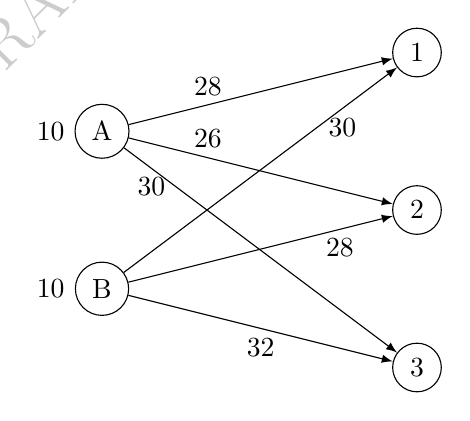
\begin{tikzpicture}[>=latex] % to get latex arrowheads

  \node[circle,draw](B) at (0,2) {B};
  \node[circle,draw](A) at (0,4) {A};
  \node[circle,draw](3) at (4,1) {3};
  \node[circle,draw](2) at (4,3) {2};
  \node[circle,draw](1) at (4,5) {1};

  \draw[->] (A) -- (1) node[above,pos=.3]{28};
  \draw[->] (A) -- (2) node[above,pos=.3]{26};
  \draw[->] (A) -- (3) node[below,pos=.1]{30};
  \draw[->] (B) -- (1) node[below,pos=.8]{30};
  \draw[->] (B) -- (2) node[below,pos=.8]{28};
  \draw[->] (B) -- (3) node[below,pos=.5]{32};

  \node[anchor=east] at (A) {10~~~~};
  \node[anchor=east] at (B) {10~~~~};

\end{tikzpicture}
\end{center}

Let $x_{ij}$ be the number of hours of instruction bidder $j$ receives
from professional golfer $i$.
  \[
     i \in \{\text{A},\text{B}\} \qquad j \in \{1,2,3\}
  \]
  The problem formulation is
\[
  \begin{array}{lrrrrrrrrrr}
    \textrm{maximize} &&&&&&&&&&\\   
    28x_{\text{A}1}&+& 26x_{\text{A}2}&+&30x_{\text{A}3}&+&30x_{\text{B}1}&+&28x_{\text{B}2}&+&32x_{\text{B}3} \\ \\
    \textrm{subject to}  &&&&&&&&&&\\
    & & & & x_{\text{A}1}&+ & x_{\text{A}2}&+ &x_{\text{A}3} & = & 10 \\
    & & & & x_{\text{B}1}&+ & x_{\text{B}2}&+ &x_{\text{B}3} & = & 10 \\
    & & & & & &  x_{\text{A}1} & + & x_{\text{B}1} & \leq & 8 \\
    & & & & & &  x_{\text{A}2} & + & x_{\text{B}2} & \leq & 8 \\
    & & & & & &  x_{\text{A}3} & + & x_{\text{B}3} & \leq & 8 \\
    \multicolumn{11}{r}{x_{ij} \geq 0 \quad \text{for}~i \in \{\text{A},\text{B}\},~j \in \{1,2,3\} }
  \end{array}
\]

The optimal solution is: bidder 1 (Emma) receives 6 hours of
instruction with Amy and 2 hours of instruction with Brian, bidder 2
(Dan) receives 4 hours of instruction with Amy, and bidder 3 (Sam)
receives 8 hours of instruction with Brian. The charity receives \$588
in revenue. A GAMS model and solution is provided in
\texttt{golf-lessons.gms}.  \emph{Note:} There are multiple optimal
solutions to this problem, so the values of the decision variables in
your solution could differ, but the value of the objective function
will be the same.
\end{solution}

% we need GAMS code for this problem, otherwise it's OK
\item \emph{A supply chain problem.} A company will produce the same
new product at two different factories, and then the product will be
shipped to two warehouses. Factory 1 can send an unlimited amount by
rail to warehouse 1 only, whereas factory 2 can send an unlimited
amount by rail to warehouse 2 only. However, independent truckers
can can be used to ship up to 50 units from each factory to a
distribution center (DC), from which up to 50 units can be shipped
to each warehouse.  The shipping cost for each alternative is shown
in the following table, along with the amounts to be produced and
the amounts needed at the warehouses.

\begin{center}
\begin{tabular}{|l|r|r|r|r|}\hline
      & \multicolumn{3}{c|}{Unit shipping cost} & \\ \cline{2-4}
      & & \multicolumn{2}{c|}{Warehouse} & \\ \cline{3-4} 
      \diagbox[width=10em]{From}{To}&  DC & WH1 & WH2 & supply \\ \hline
      Factory 1&  3 &  7 & -- & 80\\
      Factory 2&  4 &  --&  9 & 70\\
      DC       &    &  2 &  4 &   \\ \hline
      demand   &    & 60 & 90 &   \\ \hline
\end{tabular}
\end{center}

\begin{enumerate}
\item Draw the network representation of this problem as a transshipment problem.
\item Formulate the linear programming problem that minimizes total shipping cost.
\item Solve this problem using an algebraic modeling language such as GAMS.
\end{enumerate}

\begin{solution}
\bs

To make the notation easier, assign numbers to the nodes in the
network as follows: node 1 is factory 1, node 2 is factory 2, node 3
is the DC, node 4 is warehouse 1, and node 5 is warehouse 2.  Let
$x_{ij}$ be the number of products shipped from node $i$ to node $j$.

\begin{center}
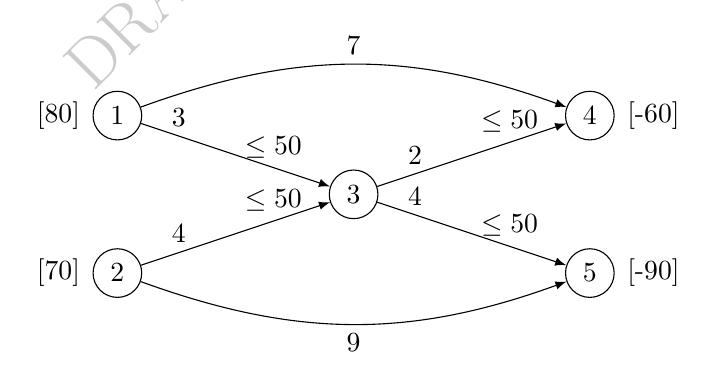
\begin{tikzpicture}[>=latex]
\node[circle,draw](f1) at (0,2) {1};
\node[circle,draw](f2) at (0,0) {2};
\node[circle,draw](dc) at (3,1) {3};
\node[circle,draw](wh2) at (6,0) {5};
\node[circle,draw](wh1) at (6,2) {4};

\node[anchor=east] at (f1) {[80]~~~~};
\node[anchor=east] at (f2) {[70]~~~~};
\node[anchor=west] at (wh1) {~~~[-60]};
\node[anchor=west] at (wh2) {~~~[-90]};

\draw[->] (f1) to [out=20,in=160]  node[above,pos=.5]{7} (wh1);
\draw[->] (f2) to [out=340,in=200] node[below,pos=.5]{9} (wh2);
\draw[->] (f1) -- (dc) node[above,pos=.2]{3} node[above,pos=.7]{$\leq 50$};
\draw[->] (f2) -- (dc) node[above,pos=.2]{4} node[above,pos=.7]{$\leq 50$};
\draw[->] (dc) -- (wh1) node[above,pos=.2]{2} node[above,pos=.7]{$\leq 50$};
\draw[->] (dc) -- (wh2) node[above,pos=.2]{4} node[above,pos=.7]{$\leq 50$};
\end{tikzpicture}
\end{center}

\[
\begin{array}{lrrrrrrrrrrl}
\textrm{minimize} & 3x_{13} &+& 4x_{23} &+& 7x_{14} &+& 9x_{25} &+& 2x_{34} &+& 4x_{35} \\
\textrm{subject to} &&&&&&& x_{13} &+& x_{14} &=& 80\\
&&&&&&& x_{23} &+& x_{25} &=& 70\\
&&&&&&& x_{34} &+& x_{14} &=& 60\\
&&&&&&& x_{25} &+& x_{35} &=& 90\\
&&&&&&&&& x_{13} & \leq & 50\\
&&&&&&&&& x_{23} & \leq & 50\\
&&&&&&&&& x_{34} & \leq & 50\\
&&&&&&&&& x_{35} & \leq & 50\\
&&& x_{13} &+& x_{23} &-& x_{34} &-& x_{35} &=& 0\\
\multicolumn{10}{r}{x_{ij}} & \geq & 0
\end{array}
\]
We note that the flow balance constraint at the DC is unnecessary
because total supply equals total demand.
\end{solution}

% re-written by hannah
\item \emph{A work-holding material for manufacturing.}  A material
compound
   is used in a manufacturing process to hold parts while
they are being machined.
  a machine. The material flows when heated and becomes solid when
  cooled. An industrial engineer must determine a method for
  maintaining the quality of the material over a four-week period,
  while minimizing cost. The engineer knows that $r_j \geq 0$ pounds
  of the material will be required in each of the four weeks,
  $j = 1, 2, 3, 4$. This demand can be met by either purchasing new
  material at cost $P$ dollars per pound or by filtering the old
  material and reusing it.  Two options are available for filtering:
   normal service, which requires 1 full week at a cost
  of $N$ dollars per pound, and expedited service, which allows
  material used during one week to be filtered by the start of the
  next week, at a cost of $Q$ dollars per pound. Currently, the
  manufacturing company has no work-holding material available.

\begin{enumerate}
\item Formulate a network flow problem that will allow the company to
  satisfy the demand for the work-holding material at minimal cost.
  You should draw a diagram of the network to help you formulate the
  problem. Note that because the company can purchase new work-holding
  material, used material can be discarded at the end of a week, if it
  is economical to do so.
	
\item Now suppose that used material may be filtered and re-used only
  once. How does the model change?
\end{enumerate}
% this was the car races problem from Bradley AMP.

\begin{solution}
  \bs Define the following variables.

  \begin{tabular}{rl}
    $x_{0j}$ & pounds (lbs) of new material purchased for the beginning of week $j$ \\
$y_{ij}$ & lbs material for expedited filtering from end of week $i$ to beginning of week $j$ \\
$z_{ij}$ & lbs material for normal filtering from end of week $i$ to beginning of week $j$ \\
$w_{i5}$ & lbs material discarded at the end of week $i$
  \end{tabular}

The network flow can be depicted as follows. Node 0 represents the beginning of the
four-week period. Nodes 1 through 4 represent weeks 1 through 4. Node 5 represents
the sink node for discarded material.

\begin{center}
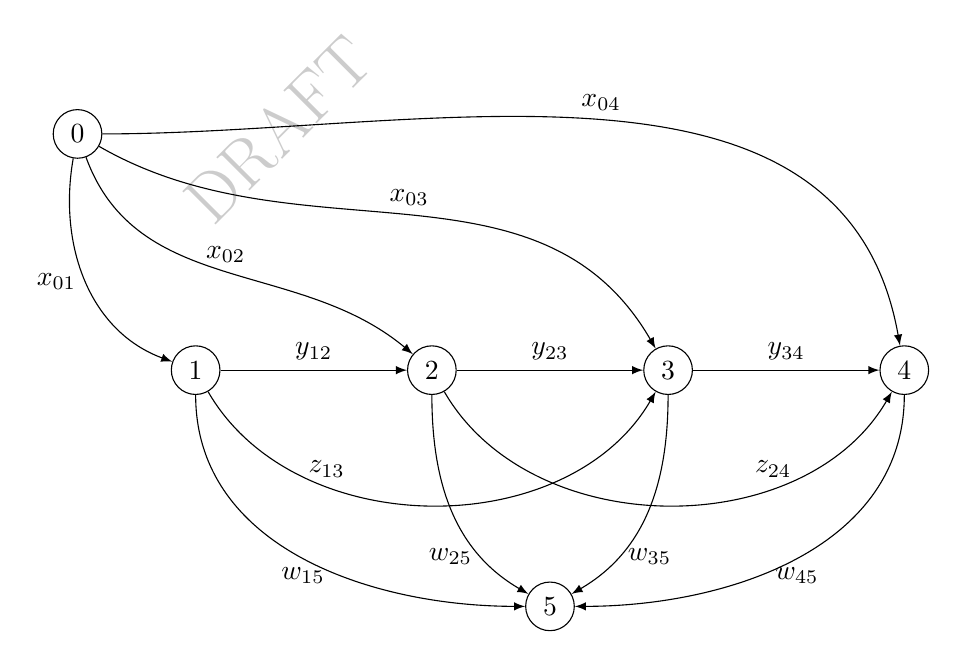
\begin{tikzpicture}[>=latex]
\node[circle,draw](0) at (-1.5,3) {0};
\node[circle,draw](1) at (0,0) {1};
\node[circle,draw](2) at (3,0) {2};
\node[circle,draw](3) at (6,0) {3};
\node[circle,draw](4) at (9,0) {4};
\node[circle,draw](5) at (4.5,-3) {5};

\draw[->] (0) to [out=260,in=160]  node[left,pos=.5]{$x_{01}$} (1);
\draw[->] (0) to [out=290,in=140]  node[above,pos=.5]{$x_{02}$} (2);
\draw[->] (0) to [out=330,in=120]  node[above,pos=.5]{$x_{03}$} (3);
\draw[->] (0) to [out=0,in=100]  node[above,pos=.5]{$x_{04}$} (4);

\draw[->] (1) to [out=0,in=180]  node[above,pos=.5]{$y_{12}$} (2);
\draw[->] (2) to [out=0,in=180]  node[above,pos=.5]{$y_{23}$} (3);
\draw[->] (3) to [out=0,in=180]  node[above,pos=.5]{$y_{34}$} (4);

\draw[->] (1) to [out=300,in=240]  node[above,pos=.3]{$z_{13}$} (3);
\draw[->] (2) to [out=300,in=240]  node[above,pos=.7]{$z_{24}$} (4);

\draw[->] (1) to [out=270,in=180]  node[below,pos=.5]{$w_{15}$} (5);
\draw[->] (2) to [out=270,in=150]  node[left,pos=.75]{$w_{25}$} (5);
\draw[->] (3) to [out=270,in=30]  node[right,pos=.75]{$w_{35}$} (5);
\draw[->] (4) to [out=270,in=0]  node[below,pos=.5]{$w_{45}$} (5);
\end{tikzpicture}
\end{center}
The mathematical programming problem is to

\[
\begin{array}{lrrrrrrrrll}
\textrm{minimize} & \multicolumn{10}{r}{P(x_{01} + x_{02} + x_{03} + x_{04}) + Q(y_{12}+y_{23}+y_{34}) +N(z_{13}+z_{24})} \\
\textrm{subject to} & x_{01} & \geq & r_1 &&&&&&&(1)\\
& x_{02}&+&y_{12}&\geq&r_2&&&&&(2)\\
& x_{03}&+&y_{23}&+&z_{13}&\geq&r_3&&&(3)\\
& x_{04}&+&y_{34}&+&z_{24}&\geq&r_4&&&(4)\\
& x_{01}&=&w_{15}&+&y_{12}&+&z_{13}&&&(5)\\
& x_{02}&+&y_{12}&=&w_{25}&+&y_{23}&+&z_{24}&(6) \\
& x_{03}&+&y_{23}&+&z_{13}&=&w_{35}&+&y_{34}&(7) \\
& x_{04}&+&y_{34}&+&z_{24}&=&w_{45}&&&(8)\\
& \multicolumn{9}{r}{x_{ij},~y_{ij},~z_{ij},~w_{ij} \geq 0~\text{for each edge $i,j$ in the network.}}
\end{array}
\]

Constraints 1 -- 4 pertain to the material requirements for weeks 1
through 4.  Constraints 5 -- 8 are the flow balance constraints. They
require that the material that enters the beginning of a week must
exit at the end of the week.

If the work-holding material can be filtered only once, then we 
require that all incoming flow on edges that represent filtering (i.e. $y_{ij}$ and
$z_{ij}$) must be routed to node 5 (the discard node). To accomplish this, one idea
is to split nodes 2 and 3 as depicted in the diagram below. All flow into nodes 2a
and 3a must be discarded, but is allowed to help satisfy the demand requirements.

\begin{center}
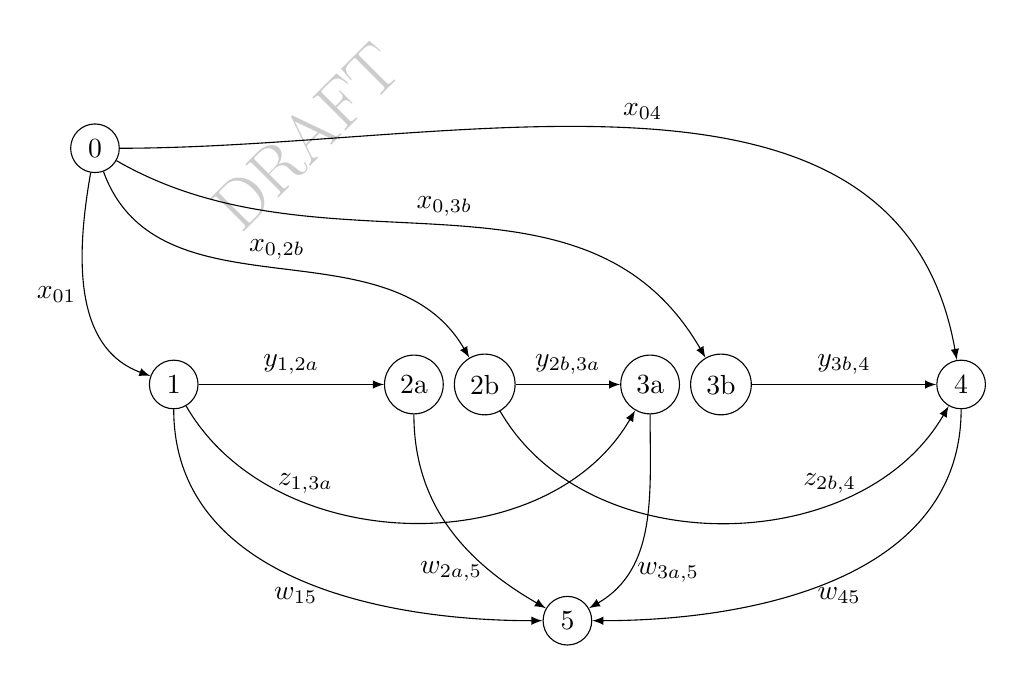
\begin{tikzpicture}[>=latex]
\node[circle,draw](0) at (-1.5,3) {0};
\node[circle,draw](1) at (-.5,0) {1};
\node[circle,draw](2a) at (2.55,0) {2a};
\node[circle,draw](2b) at (3.45,0) {2b};
\node[circle,draw](3a) at (5.55,0) {3a};
\node[circle,draw](3b) at (6.45,0) {3b};
\node[circle,draw](4) at (9.5,0) {4};
\node[circle,draw](5) at (4.5,-3) {5};

\draw[->] (0) to [out=260,in=160]  node[left,pos=.5]{$x_{01}$} (1);
\draw[->] (0) to [out=290,in=120]  node[above,pos=.5]{$x_{0,2b}$} (2b);
\draw[->] (0) to [out=330,in=120]  node[above,pos=.5]{$x_{0,3b}$} (3b);
\draw[->] (0) to [out=0,in=100]  node[above,pos=.5]{$x_{04}$} (4);

\draw[->] (1) to [out=0,in=180]  node[above,pos=.5]{$y_{1,2a}$} (2a);
\draw[->] (2b) to [out=0,in=180]  node[above,pos=.5]{$y_{2b,3a}$} (3a);
\draw[->] (3b) to [out=0,in=180]  node[above,pos=.5]{$y_{3b,4}$} (4);

\draw[->] (1) to [out=300,in=240]  node[above,pos=.3]{$z_{1,3a}$} (3a);
\draw[->] (2b) to [out=300,in=240]  node[above,pos=.7]{$z_{2b,4}$} (4);

\draw[->] (1) to [out=270,in=180]  node[below,pos=.5]{$w_{15}$} (5);
\draw[->] (2a) to [out=270,in=150]  node[left,pos=.75]{$w_{2a,5}$} (5);
\draw[->] (3a) to [out=270,in=30]  node[right,pos=.75]{$w_{3a,5}$} (5);
\draw[->] (4) to [out=270,in=0]  node[below,pos=.5]{$w_{45}$} (5);
\end{tikzpicture}
\end{center}

Now the objective function and demand requirements are
\[
\begin{array}{lrrrrrrrrll}
\textrm{minimize} & \multicolumn{10}{r}{P(x_{01} + x_{0,2b} + x_{0,3b} + x_{04}) + Q(y_{1,2a}+y_{2b,3a}+y_{3b,4}) +N(z_{1,3a}+z_{2b,4})} \\
\textrm{subject to} & x_{01} & \geq & r_1 &&&&&&&(1)\\
& x_{02}&+&y_{1,2a}&\geq&r_2&&&&&(2)\\
& x_{03}&+&y_{2b,3a}&+&z_{1,3a}&\geq&r_3&&&(3)\\
& x_{04}&+&y_{3b,4}&+&z_{2b,4}&\geq&r_4&&&(4)\\
\end{array}
\]
We also need flow balance constraints for nodes 1,2a,2b,3a,3b,4, and
the non-negativity constraints.

\end{solution}

% re-written by hannah
\item \emph{Laundering clean-room garments.} A medical device company
  uses a cleanroom to assemble and inspect many of its
  products. Because the purpose of a cleanroom is to limit pollutants
  and contaminants, there are strict guidelines that must be
  followed. At this company, each employee and visitor who enters the
  cleanroom must wear a clean lab coat. As a result, there must be
  enough clean lab coats at the beginning of each day for all
  employees and visitors who enter the cleanroom. The company
  outsources cleaning to an laundry service. Normal laundry takes one
  full day at a cost of \$2.25 per lab coat. Overnight laundry service
  can be done at a cost of \$5 per lab coat. Under normal
  circumstances, the current supply of 40 lab coats is sufficient for
  complete dependence upon the normal laundry service. However, the
  normal laundry service will not be sufficient for the next three
  days due to a training program and audit that will take place. It is
  known that the requirements for the next three days will be 25, 35,
  and 30 lab coats. It is now mid-afternoon on the day before the
  training program and audit. 15 lab coats are clean, and 25 are ready
  for laundry. It is against clean-room protocol to have used lab
  coats remain at the company overnight. The clean-room will be closed
  on the day after the training program and audit, so all used lab
  coats on the third day can be sent to normal laundry. An industrial
  engineer wants to determine a plan for laundering that will minimize
  total cost while satisfying demand and respecting the clean-room
  protocol.

  Interpret this problem as one of network flow.  Draw the network and
  formulate the LP (i.e. the decision variables, the objective
  function, and the constraints.)
% this was the napkin laundering problem from AMP.

\begin{solution}
\bs Define the following variables.

\begin{tabular}{rl}
$x_i$ & number of garments sent to regular laundry at the end of day $i$ \\
$y_i$ & number of garments sent to overnight service at the end of day $i$ \\
$z_i$ & number of clean (unused) garments at the end of day $i$
\end{tabular}

The network flow diagram can be depicted as shown below. Node 0 represents the
current day (before the three-day event). Nodes 1, 2, and 3 represent the next
three days of the higher-than-usual demand. Node 4 represents the day following
the three-day event. For example, the flow labeled $x_0$ represents the garments
that are sent to the normal laundry service today. Those garments will be
available at the beginning of day 2.

\begin{center}
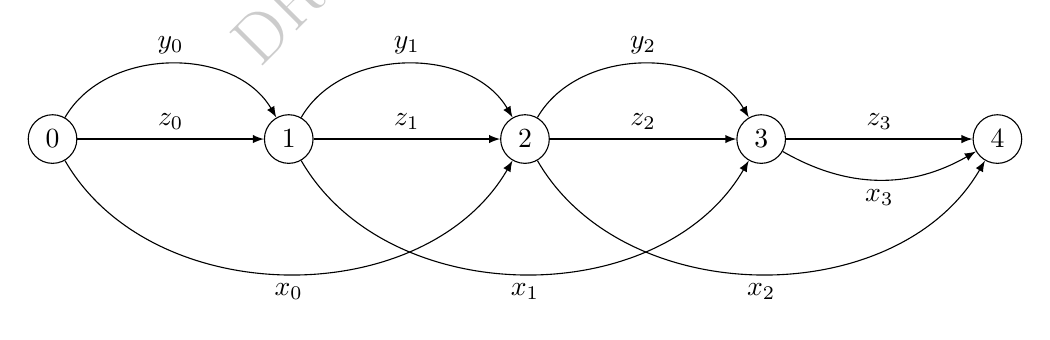
\begin{tikzpicture}[>=latex]
\node[circle,draw](0) at (-3,0) {0};
\node[circle,draw](1) at (0,0) {1};
\node[circle,draw](2) at (3,0) {2};
\node[circle,draw](3) at (6,0) {3};
\node[circle,draw](4) at (9,0) {4};

\draw[->] (0) to [out=0,in=180]  node[above,pos=.5]{$z_0$} (1);
\draw[->] (1) to [out=0,in=180]  node[above,pos=.5]{$z_1$} (2);
\draw[->] (2) to [out=0,in=180]  node[above,pos=.5]{$z_2$} (3);
\draw[->] (3) to [out=0,in=180]  node[above,pos=.5]{$z_3$} (4);

\draw[->] (0) to [out=60,in=120]  node[above,pos=.5]{$y_0$} (1);
\draw[->] (1) to [out=60,in=120]  node[above,pos=.5]{$y_1$} (2);
\draw[->] (2) to [out=60,in=120]  node[above,pos=.5]{$y_2$} (3);

\draw[->] (0) to [out=300,in=240]  node[below,pos=.5]{$x_0$} (2);
\draw[->] (1) to [out=300,in=240]  node[below,pos=.5]{$x_1$} (3);
\draw[->] (2) to [out=300,in=240]  node[below,pos=.5]{$x_2$} (4);
\draw[->] (3) to [out=330,in=210]  node[below,pos=.5]{$x_3$} (4);
\end{tikzpicture}
\end{center}

The formulation of the mathematical programming problem is
\[
\begin{array}{lrrrrrrrrrrll}
\textrm{minimize} & \multicolumn{11}{r}{5\left(y_0+y_1+y_2\right) + 2.25\left(x_0+x_1+x_2+x_3\right)}&\\
\textrm{subject to} & y_0&+&z_0&+&x_0&=&40&&&&&(1) \\
& y_0&+&z_0&=&y_1&+&z_1&+&x_1&&&(2) \\
& y_1&+&z_1&+&x_0&=&y_2&+&z_2&+&x_2&(3) \\
& y_2&+&z_2&+&x_1&=&x_3&+&z_3&&&(4)\\
& y_0&+&z_0&\geq&25&&&&&&&(5)\\
&y_1&+&z_1&+&x_0&\geq&35&&&&&(6)\\
&y_2&+&z_2&+&x_1&\geq&30&&&&&(7)\\
&y_0&+&x_0&\geq&25&&&&&&&(8)\\
&y_1&+&x_1&\geq&25&&&&&&&(9)\\
&y_2&+&x_2&\geq&35&&&&&&&(10)\\
&x_3&\geq&30&&&&&&&&&(11)\\
&\multicolumn{11}{r}{x_i,y_i,z_i \geq 0}&
\end{array}
\]
Constraints 1 -- 4 are flow balance constraints for nodes 0, 1, 2, and 3,
respectively. Constraints 5, 6, and 7 are the requirements for the number
of clean garments during the three-day event. Constraints 8 -- 11 model
the clean-room protocol that used garments must be sent to a laundry service
(either normal or overnight) at the end of the day. Note that at the end
of day 3, it would not make sense to use the overnight laundry service.

\end{solution}

\subsubsection*{Integer Programming}
% this problem is OK.
\item \emph{Discrete purchases.} Sam is considering purchasing some
  combination of a new car, a washer, a dryer, and a high-definition
  television (HDTV). For practical reasons, Sam knows that he can only
  buy the dryer if he also buys the washer. It could still make sense
  to buy the washer without the dryer because Sam could dry his
  clothes on a clothesline. Due to political reasons with Sam's
  spouse, he can only purchase the HDTV if he does not purchase the
  car. Taking everything into consideration, Sam has estimated the
  values for each item. The item utilities (converted to dollars) and
  purchase prices in dollars are shown in the table below.  Sam's
  total budget is \$16,000. Formulate a binay integer programming
  problem to maximize Sam's estimated value while respecting the
  practicality, spouse, and budget constraints mentioned above.

\begin{center}
\begin{tabular}{lcc}
Item    &  Estimated value  & Price   \\  \hline
car     &   \$9,500   &  \$12,000 \\
washer  &   \$3,000   &  \$2,000  \\
dryer   &   \$3,000   &  \$2,000  \\
HDTV    &   \$5,000   &  \$3,000  \\
\end{tabular}
\end{center}

\begin{solution}
\bs

\[ \text{Let}~x_j = \begin{cases}
1 \quad \text{if item $j$ is purchased}\\
0 \quad \text{otherwise} \end{cases}
\]

where the index $j = 1,2,3,4$ corresponds to the car, washer, dryer,
and HDTV. The problem is to 
\[
\begin{array}{lrrrrrrrrl}
\textrm{maximize}   & 9.5x_1& +& 3x_2&+& 3x_3 &+& 5x_4 & & \\
  \textrm{subject to} & 12x_1& +& 2x_2&+& 2x_3 &+& 3x_4 & \leq & 16 \\
                    &&&&&& &x_3 & \leq & x_2 \\
                    &&&&& x_1 & + & x_4 &\leq& 1 \\
\multicolumn{8}{r}{x_j}&  \in & \{0,1\}
\end{array}
\]
\end{solution}

% re-written by hannah
\item \emph{A set covering problem.}  A general merchandise retailer
  is planning to expand into a new metropolitan area comprised of
  seven cities. The following table shows the distance (in miles)
  between each city.

\begin{center}
\begin{tabular}{l|ccccccc}
& \multicolumn{7}{c}{To} \\
From & City 1 & City 2 & City 3 & City 4 & City 5 & City 6 & City 7\\ \hline
City 1 & 0 & 15 & 20 & 38 & 20 & 28 & 22 \\
City 2 & 15 & 0 &  5 & 23 & 16 & 12 & 10 \\
City 3 & 20 & 5 & 0 & 18 & 12 & 13 & 14 \\
City 4 & 38 & 23 & 18 & 0 & 31 & 19 & 27 \\
City 5 & 20 & 16 & 12 & 31 & 0 & 7 & 19 \\
City 6 & 28 & 12 & 13 & 19 & 7 & 0 & 22 \\
City 7 & 22 & 10 & 14 & 27 & 19 & 22 & 0 \\
\end{tabular}
\end{center}

The company assumes that customers will only visit a retail location
if it is within 15 miles of the city in which the customer
lives. Using this information, the company would like to construct the
fewest number of stores while ensuring that they can serve every
customer in the metropolitan area. Formulate an integer programming
model to determine the cities where retail locations should be
constructed.

\begin{solution}
\bs
\begin{equation*}
\text{Let $x_i$} = 
\begin{cases}
  1 & \text{if a retail location is constructed in city $i$,}\\
  0 & \text{otherwise.}
\end{cases}
\end{equation*}

To model the requirement that there is at least one retail location within
15 miles of city 1, we require that $x_1 + x_2 \geq 1$. The full
problem formulation is
\[
\begin{array}{lrrrrrrrrrrrrl}
\textrm{minimize} & \sum_{i=1}^{7} x_i & & & & & & \\
\textrm{subject to} && & & & & & & & x_1 & + & x_2 & \geq & 1 \\
& & & x_1 & + & x_2 & + & x_3 & + & x_6 & + & x_7 & \geq & 1 \\ & &  & x_2 & + & x_3 & + & x_5 & + & x_6 & + & x_7 & \geq & 1 \\
& &  & & & & & &  &  &  & x_4 & \geq & 1 \\
& & & &  & &  & x_3 & + & x_5 & + & x_6 & \geq & 1 \\
& & & &  & x_2 & + & x_3 & + & x_5 & + & x_6 & \geq & 1 \\
& & & & & & & x_2 & + & x_3 & + & x_7 & \geq & 1 \\
\multicolumn{14}{r}{x_i \in \{0,1\} \quad i = 1,\ldots,7}
\end{array}
\]
\end{solution}

% re-written by hannah
\item \emph{A set partitioning problem.} A DSL (Digital Subscriber
  Line) Internet service provider is determining where to construct
  three central offices in a city. A customer’s DSL connection works
  better when they are near a central office, so customers that live
  close to a new central office will experience faster Internet
  speeds. The city is divided into six geographical regions, and an
  industrial engineer must decide which regions should have central
  offices. The engineer must also determine which regions each central
  office will serve. The following table indicates the average
  internet speed in a region, depending on the region of the central
  office that provides service.

\begin{center}
\begin{tabularx}{3.75in}{>{\setlength\hsize{.9in}\centering}Y|ZZZZZZ}
\multirow{2}{.9in}{location of central office} & \multicolumn{6}{c}{avg internet speed in region} \\
& 1 & 2 & 3 & 4 & 5 & 6\\ \hline
1 & 45 & 35 & 30 & 25 & 10 & 12\\
2 & 35 & 45 & 20 & 20 & 25 & 18\\
3 & 30 & 20 & 45 & 30 & 15 & 25\\
4 & 25 & 20 & 30 & 45 & 12 & 27\\
5 & 10 & 25 & 15 & 12 & 45 & 30\\ 
6 & 12 & 18 & 25 & 27 & 30 & 45\\ 
\end{tabularx}
\end{center}

Formulate an integer programming model to determine the regions in
which central offices are located and the regions to which each
central is assigned so that the average internet speed in the city is
maximized.

\begin{solution}
  \bs Let $a_{ij}$ be the data describing the average internet speed
  in region $j$ when served by a central office in region $i$. Also,
  let the decision variables be

\begin{equation*}
\text{$x_{ij}$} = 
\begin{cases}
    1 & \text{if central office in region $i$ provides service to region $j$}\\
    0 & \text{otherwise.}
\end{cases}
\end{equation*}
and
\begin{equation*}
\text{$y_i$} = 
\begin{cases}
    1 & \text{if central office is constructed in region $i$}\\
    0 & \text{otherwise.}
\end{cases}
\end{equation*}

The problem is to
\[
\begin{array}{lll}
\textrm{maximize} & \multicolumn{2}{c}{\displaystyle\sum_{i=1}^6 \sum_{j=1}^6 a_{ij}x_{ij}} \\
\textrm{subject to} & \displaystyle\sum_{i=1}^6 y_i &= 3  \\
& \displaystyle\sum_{i=1}^{6} x_{ij} &= 1~\text{for all $j$}\\ 
& x_{ij} &\leq y_i~\text{for all $i$ and $j$} \\
& \multicolumn{2}{r}{ x_{ij} \in \{0,1\}} \\
& \multicolumn{2}{r}{ y_i \in \{0,1\}} \\
& \multicolumn{2}{r}{ i = 1,\ldots,6} \\
& \multicolumn{2}{r}{ j = 1,\ldots,6}
\end{array}
\]
The objective function will maximize the average Internet speed of the
six regions. We could include the constant 1/6, which would change the
value of the objective function, but not the values of the decision
variables.
\end{solution}

% re-written by hannah
\item \emph{A problem with a fixed charge.}  A bicycle manufacturing
  company can produce three types of bikes: mountain bikes, road
  bikes, and fat bikes. The company rents specific machinery for
  producing each type of bike. It costs \$150 per week to rent
  machinery for mountain bikes, \$250 per week to rent machinery for
  road bikes, and \$300 per week to rent machinery for fat bikes. A
  maximum of 120 hours of labor and \num{11000} pounds of material
  (aluminum) are available each week for production. The material
  and labor requirements to produce one unit of each type of bike are
  shown in the table below. The unit variable cost and the unit
  selling price for each type of bike are also shown.

\vspace{.1in}
\begin{tabulary}{5.4in}{LRRRR}
& Labor (hours) 
& Material (pounds) 
& Variable cost 
& Selling price \\ \hline
Mtn bike & 2.5 & 28 & \$350 & \$550 \\
Road bike & 7 & 25 & \$420 & \$800 \\
Fat bike & 4.5 & 36 & \$680 & \$\num{1200}
\end{tabulary}
\vspace{.1in}

The machinery needed to produce a specific type of bike is only rented
if that type of bike is produced. Assume that the company can sell all
of the bikes that it produces, regardless of type.  Formulate a mixed
integer linear programing problem to determine the weekly production
quantities of mountain bikes, road bikes, and fat bikes that will
maximize profit.

\begin{solution}
  \bs Let the decision variables $x_1,x_2,x_3$ be the number of
  mountain bikes, road bikes, and fat bikes, respectively, to produce
  each week. Machinery rental costs are only incurred if bicycles of that
  particular type are produced. We introduce binary decision variables
  $y_i$ to apply the machinery rental costs when production $x_i$ is
  positive.
\[
\text{Let $y_i$} = 
\begin{cases}
1 & \text{if $x_i > 0$} \\
0 & \text{otherwise}
\end{cases}
\quad i = 1,2,3.
\]
The mathematical formulation of the Integer Programming problem is
\[
\begin{array}{lrrrrrrl}
\textrm{maximize} &   & 550x_1 & + & 800x_2 & + & \num{1200}x_3 & \\
& - & 350x_1  & - & 420x_2 & - & 680x_3  & \\
& - & 150y_1& - & 250y_2&- & 300y_3& \\
& & & & & & &\\
\textrm{subject to} & 2.5x_1 & + & 7x_2 & + & 4.5x_3 & \leq & 120 \\
& 28x_1 & + & 25x_2 & + & 36x_3 & \leq & \num{11000} \\
& & & & & x_1 & \leq & My_1 \\
& & & & & x_2 & \leq & My_2 \\
& & & & & x_3 & \leq & My_3 \\
\end{array}
\]
where $M$ is a large number, $x_i \geq 0$, $x_i$ are integer-valued, 
$y_i \in \{0,1\}$, and $i = 1,2,3$.
\end{solution}

% re-written by hannah
\item \emph{A maxi-min problem.} A college student has received a \$50
  gift and is interested in four different investment options. One
  of three possible random events will occur in the next year that
  will impact the return on the investments. The return for each
  dollar invested in each of the four options for each event is
  shown in the table below. For example, if the student invests \$1 in
  option 3 and event B occurs, the student will receive a return of
  \$7.  Investment amounts must be in increments of \$1. The student is
risk-averse; his objective is to maximize the minimum return.
  Formulate an integer programming problem and obtain a
  solution.  \emph{Hint:} The decision variables are the amounts to
  invest in each option. Introduce another variable (say $w$) that
  represents the minimum return. Then, if $w$ is the minimum return,
  the actual return for each possible outcome must be greater than or
  equal to $w$.)

\begin{tabular}{c|rrr}
	& \multicolumn{3}{c}{event}\\
	option & A & B & C \\ \hline
	1 & -4 & 6 & 5 \\
	2 & 4 & -2 & -11 \\
	3 & -5 & 7 & 12 \\
	4 & 12 & 6 & -4
\end{tabular}
\vspace{.2in}

\begin{solution}
	\bs Let the decision variables $x_i$ represent the amounts to invest
	in each option, where $i = 1,2,3,4$. Also, let $w$ represent
	the minimum return among the three events. The student wants to
	
	\[
	\begin{array}{lrrrrrrrrrrr}
	\textrm{maximize} & w & \multicolumn{10}{c}{} \\
	\textrm{subject to} & -4x_1 & + & 4x_2 & - & 5x_3 & + & 12x4 &-&50&\geq & w \\
	& 6x_1 & - & 2x_2 & + & 7x_3 & + & 6x4 &-&50&\geq & w \\
	& 5x_1 & - & 11x_2 & + & 12x_3 & - & 4x4 &-&50&\geq & w \\
	&  & & x_1 & + & x_2 & + & x_3 &+&x_4& = & 50 \\
	\end{array}
	\]
	where $x_i$ is integer-valued and non-negative, and $w$ is
        unrestricted.  An implementation and solution is provided in
        the files \texttt{maxi-min.gms} and \texttt{maxi-min.lst}. The
        solution indicates that the student should invest \$24 in
        option 3 and \$26 in option 4 for a guaranteed minimum return
        of \$134.

\end{solution}

% re-written by hannah
\item \emph{Modeling with binary variables.} This problem (slightly
  altered) appears in~\cite{bradley:1977}, an excellent book that is
  freely available on-line. A business sells video games and
  movies. For each video game sold, the business earns a profit of
  \$1. For each movie sold, the business earns a profit of \$2. The
  store manager, who is a bit quirky, has imposed the following
  restrictions on customers' purchases.

\begin{compactenum}[i)]
\item There is a limit of eight items (total) per customer.
\item The number of movies purchased minus the number of video games
purchased cannot exceed 2.
\item The number of video games purchased minus the number of movies
purchased cannot exceed four.
\item A customer can purchase zero, one, four, or six video games. No
  other quantities of video games are allowed. There is no such
  restriction on the quantity of movies.
\end{compactenum}

The manager would like to determine the combination of purchases by a
customer that will maximize profit. Letting $x_1$ and $x_2$ represent
the quantities of video games and movies, respectively, the problem
can be formulated as follows.

\[
\begin{array}{lrrrrrrl}
\textrm{maximize} &   & z & = & x_1 & + & 2x_2 & \\
\textrm{subject to} & & & x_1 & + & x_2 & \leq & 8 \\
& & & -x_1 & + & x_2 & \leq & 2 \\
& & & x_1 & - & x_2 & \leq & 4 \\
& & & & & x_2 & \geq & \text{0, and integer} \\
& & & & & x_1 & = & \text{0,1,4, or 6} \\
\end{array}
\]

\begin{enumerate}
\item Reformulate the problem as an equivalent integer linear
  program.\label{ex:ip}
\item How would your answer to part \ref{ex:ip} change if the
  objective function was instead
\[ \text{maximize~} z = x_1^2 + 2x_2\text{?} \] \label{ex:quad}
\end{enumerate}

\begin{solution} 
\bs Introduce the following binary variables. Let
\[ y_i = \begin{cases}
1 \quad \text{if}~ x_1 = i \quad i \in \{0,1,4,6\}\\
0 \quad \text{otherwise}
\end{cases}
\]

Now the binary integer programming formulation is
\[
\begin{array}{lrrrrrrrrl}
\textrm{maximize}   &&& y_1 & + & 4y_4 & + & 6y_6 & + & 2x_2 \\
\textrm{subject to} & y_0 & + & y_1 & + & y_4 & + & y_6 & = & 1 \\
& y_1 & + & 4y_4 & + & 6y_6 & + & x_2 & \leq & 8\\
& -y_1 & - & 4y_4 & - & 6y_6 & + & x_2 & \leq & 2\\
& y_1 & + & 4y_4 & + & 6y_6 & - & x_2 & \leq & 4\\
\multicolumn{8}{r}{x_2}& \geq & 0 ~\text{and integer}\\
\multicolumn{8}{r}{y_0,y_1,y_4,y_6}& \in & \{0,1\}
\end{array}
\]
For part \ref{ex:quad}, change the coefficients on the $y_i$
variables in the objective function only to be the squares,
i.e. $16y_4$ and $36y_6$. Note that by using this technique the
objective function is transformed from a quadratic to a linear function
of the variables.
\end{solution}

\begin{comment}
% Let's hold off on this problem for now. This problem should be explained
% in the chapter.
\item \emph{Scheduling a sports league.} An amateur hockey league is
  being formed among four cities in northern Minnesota. The cities
  with teams are Bemidji, Park Rapids, Crookston, and Detroit
  Lakes. The league is to be split into two divisions, A and B. Each
  division will have two teams. Each team is to play four away games
  against the opponent in their own league and two away games against
  opponents in the other league. We can represent this with the
  following ``away-game matrix''.

\begin{center}
\begin{tabular}{rrr}
    & A & B\\
  A & 4 & 2\\
  B & 2 & 4
\end{tabular}
\end{center}

The distances between cities are:

\begin{center}
\begin{tabular}{lrrrr}
  & \multicolumn{4}{c}{Distance in miles} \\
            & Bemidji & Park Rapids & Crookston & Detroit Lakes \\
Bemidji     &  0  &     47   &      87   &     85\\
Park Rapids  & 47  &     0    &      114  &     39\\
Crookston   & 87  &     114  &      0    &     92\\
Detroit Lakes& 85  &     39   &      92   &     0
\end{tabular}
\end{center}

Find an assignment of teams to divisions that minimizes total league
travel.

\begin{solution}
\bs The league structure that minimizes total travel is to assign
Bemidji and Crookston to one division, and assign Detroit Lakes and
Park Rapids to the other division. My AMPL output is shown below.

\begin{Verbatim}[samepage=true]
ampl: include '/home/darin/Dropbox/isye/ie1101/ampl/options.run';
ampl: model '/home/darin/Dropbox/isye/ie1101/hw/realignment.mod';
ampl: data '/home/darin/Dropbox/isye/ie1101/hw/realignment-mn.dat';
ampl: solve;
CPLEX 12.7.1.0: sensitivity
CPLEX 12.7.1.0: optimal integer solution; objective 2360
36 MIP simplex iterations
0 branch-and-bound nodes

suffix up OUT;
suffix down OUT;
suffix current OUT;
ampl: display x;
x :=
bemidji      divA   1
bemidji      divB   0
crookston    divA   1
crookston    divB   0
detroitlakes divA   0
detroitlakes divB   1
parkrapids   divA   0
parkrapids   divB   1
;  
\end{Verbatim}
\end{solution}
\end{comment}

\subsubsection*{Deterministic Dynamic Programming}

\item \emph{An optimal assignment of resources.} 
The number of crimes in each of a city's three
  precincts depends on the number of police cars assigned to each
  precinct. The number of crimes is shown in the table below. Three
  patrol cars are available. Use dynamic programming to determine how
  many patrol cars should be assigned to each precinct so that the
  total number of crimes is minimized.

  \begin{center}
  \begin{tabularx}{3.5in}{r|XXXX}
    & \multicolumn{4}{c}{No. of patrol cars assigned to precinct} \\
    &0 & 1 & 2 & 3 \\ \hline
    precinct 1 & 14 & 10 & 7 & 4 \\
    precinct 2 & 25 & 19 & 16 & 14 \\
    precinct 3 & 20 & 14 & 11 & 8
  \end{tabularx}
\end{center}

\begin{solution}
  \bs A natural representation for dynamic programming is that the
  stage is the precinct and the state is the number of patrol cars
  remaining. Let $x_i$ represent the number of cars to assign to
  precinct $i$, $i = 1,2,3$. With one precinct to go it makes sense to
  assign all remaining cars. In this stage I am assigning cars to
  precinct 3.

  \begin{tabular}{rrrr}
    state & $x_3$ & cost & $x_3^{\ast}$ \\ \hline
    0 & 0 & 20 & 0 \\
    1 & 1 & 14 & 1 \\
    2 & 2 & 11 & 2 \\
    3 & 3 & 8 & 3
  \end{tabular}

  With two precincts to go, we are assigning cars to precinct 2.

  \begin{tabular}{llccll}
    state & $x_2$ & cost & cost-to-go & total & $x_2^{\ast}$ \\ \hline
    0 & 0 & 25 & 20 & 45 & 0 \\ \hline

    \multirow{2}{*}{1} & 0 & 25 & 14 & $39^{\ast}$ & \multirow{2}{*}{0} \\
          & 1 & 19 & 20 & 39 &  \\ \hline

    \multirow{3}{*}{2} & 0 & 25 & 11 & 36 & \multirow{3}{*}{1} \\
          & 1 & 19 & 14 & 33$^{\ast}$ &  \\
          & 2 & 16 & 20 & 36 & \\ \hline

    \multirow{4}{*}{3} & 0 & 25 & 8 & 33 & \multirow{4}{*}{1}\\
    & 1 & 19 & 11 & $30^{\ast}$ &  \\
    & 2 & 16 & 14 & 30 & \\
    & 3 & 14 & 20 & 34 & 
  \end{tabular}

  With three precincts to go we are assigning cars to precinct 1. At this
  stage no cars have been assigned.

  \begin{tabular}{llrcll}
    state & $x_1$ & cost & cost-to-go & total & $x_1^{\ast}$ \\ \hline
    \multirow{4}{*}{3} & 0 & 14 & 30 & 44 & \multirow{4}{*}{1} \\
          & 1 & 10 & 33 & $43^{\ast}$ & \\
          & 2 & 7 & 39 & 46 & \\
          & 3 & 4 & 45 & 49 &
  \end{tabular}

  The optimal solution is to assign 1 car to each of the three
  precincts for a total of 43 crimes. You may have selected a
  different sequence of precincts for the stages, but the solution
  should be the same.
\end{solution}

\subsubsection*{Deterministic Inventory Models}

% written by Emily
% deterministic inventory model
% to replace IMS problem 5 from ch 10
\item \emph{Ordering lumber.}  Building Builders, a construction
  company, always has a full schedule of building projects.  One of
  the most important resources required for their projects is
  lumber. To complete their projects, Building Builders has a constant
  demand for lumber of \num{5000} board feet per day.  There is a
  \$300\ delivery fee every time the company orders more lumber. It
  costs \$0.02\ per week for the company to store each unused board
  foot (7 days in one week). Every order has a lead time of 2 days to
  account for order processing and delivery time.

\begin{enumerate}
\item What is the optimal order quantity (in board feet) for Building
  Builders?
\item How frequently should Building Builders order to replenish the
  lumber supply?
\item Building Builders currently has space to store \num{35000} board
  feet of lumber. Should they invest in more space to store lumber?
  Why or why not?
\item What is the reorder point?
\end{enumerate}

\begin{solution}
  \bs The cost per order is $C_0=\$300$, the holding cost is
  $C_h=\$.02$ per board foot per week, the lead time is $m=2$ days,
  the demand rate is $D=\num{5000}$ board feet per day, and there are
  7 days in a week.  The demand per week is
  \[\num{5000} ~\text{board feet per day} \times 7 ~\text{days per
      week} = \num{35000} ~\text{board feet per week}\] Using the
  formula for economic order quantity,
\[ Q^{\ast} = \sqrt{\frac{2DC_o}{C_h}} = \sqrt{\frac{2(\num{35000})(300)}{0.02}} = \num{32404}~\text{board feet.} \]

The cycle time associated with the economic order quantity is
\[ T^{\ast} = \frac{Q^{\ast}}{D} = \frac{\num{32404}}{\num{5000}} = 6.5 ~\text{days.} \]

No, Building Builders should not invest in more space to store lumber
because the economic order quantity of \num{32404} board feet is less
than the current storage space capacity of \num{35000} board feet.

The lead time is 2 days and the usage rate per day is \num{5000} board
feet, so the reorder point is $2 \times \num{5000} = \num{10000}$
board feet.
\end{solution}


\end{enumerate}
%%% Local Variables:
%%% TeX-master: "main"
%%% End:

\chapter{Probabilistic Models}

\section{Modeling with Probability Distributions}

% a discussion on binomial distribution.
The normal rate of infection of a certain disease in cattle is
25\%.  Each animal becomes infected (or not) independently of other
animals.  A team of veterinarians would like to test a new
vaccine. Which of the following two scenarios, \ref{sc1} or \ref{sc2},
provides more evidence that the vaccine is effective.  \emph{Hint:}
Compute the probability that each scenario would occur under the
hypothesis that the vaccine has no effect whatsoever.
\begin{enumerate}[A)]
\item 10 animals are vaccinated and none of them become infected. \label{sc1}
\item 17 animals are vaccinated. At most one of the animals becomes infected. \label{sc2}
\end{enumerate}

Let $X$ be the number of animals infected under the assumption that
the vaccine is worthless.  Under scenario \ref{sc1},
\[ X \sim \text{Binomial}(n=10,p=.25) \]
\[ P(X = 0) = {10 \choose 0} .25^0 .75^{10} = .0563 \]
Under scenario \ref{sc2}, 
\[ X \sim \text{Binomial}(n=17,p=.25) \]
\begin{align*} P(X \leq 1) &= P(X=0) + P(X=1) \\
                 &= \sum_{x=0}^1 {17 \choose x} .25^x .75^{17-x} \\
                 &= .0501
\end{align*}
In the absence of a working vaccine, scenario \ref{sc2} is less likely to occur,
and so it provides a better test of the effectiveness of the vaccine.


% use this section to illustrate modeling with a poisson rv
At a facility that manufactures recreational sports
  vehicles (ATVs), each vehicle is subjected to a final
  inspection. The rate of defects during final inspection is
  $\lambda=1.5$ defects per vehicle.
\begin{enumerate}
\item What is an appropriate probability distribution to model the
number of defects? \label{atv1}
\item What proportion of vehicles have more than 2 defects? \label{atv2}
\item Management has set a new goal that the proportion
of vehicles with no defects is .5. What rate $\lambda$ would
achieve this goal? \label{atv3}
\end{enumerate}

We are interested in the number of defects, which is discrete.
The Poisson distribution makes sense because it is commonly used
for count data. Moreover, we are given information for a single
parameter, and the Poisson distribution has a single parameter.
If we let the random variable $X$ represent the number of defects
per vehicle, then a reasonable distribution is
\[ X \sim \text{Poisson}(\lambda=1.5) \]
For part~\ref{atv2},
\begin{align*}
P(X>2) &= 1 - P(X \leq 2)\\
       &= 1 - \sum_{x=0}^2 \frac{e^{-\lambda}\lambda^x}{x!}\\
       &= 0.191
\end{align*}
For part \ref{atv3}, management's goal is that $P(X=0)=0.5$, or
\[ P(X=0) = \frac{e^{-\lambda}\lambda^0}{0!} = e^{-\lambda}=0.5 \]
Then
\[ \lambda = -\ln{0.5} = 0.693 \]

%% using poisson distribution and binomial distribution, and independence
The number of bacteria colonies of a certain type in samples of
polluted water has a Poisson distribution with a mean of 2 per cubic
centimeter. If four 1--cubic--centimeter samples are independently
selected from this water, find the probability that at least one
sample will contain one or more bacteria colonies.

Let $X$ be a random variable that represents the number of bacteria
colonies in a 1 cm$^3$ sample of the polluted water. From the problem
description,
\[ X \sim \text{Poisson}(\lambda = 2) \]
First let's find the probability that any particular sample will contain
at least one colony.
\begin{align*}
  P(X \geq 1) &= 1 - P(X=0)\\
              &= 1 - \frac{e^{-\lambda}\lambda^0}{0!}\\
              &= 1 - e^{-2}\\
  &= .865
\end{align*}
Now, the four samples are independent and the the probability that
a sample contains one or more colonies is the same for each sample.
Let $Y$ be a random variable that represents the number of samples
that contain one or more colonies. Then
\[ Y ~ \sim \text{Binomial}(n=4, p=0.865) \]
and we want to know $P(Y \geq 1)$.
\begin{align*}
  P(Y \geq 1) &= 1 - P(Y = 0)\\
              &= 1 - {4 \choose 0} (.865)^0 (1 - .865)^4 \\
  &= 0.9997
\end{align*}

% discussion on the Normal distribution
A refinery makes two grades of gasoline, regular and premium.  The
advertised octane ratings are 87 for regular gasoline and 89 for
premium gasoline.  The quality engineer at the refinery asks for 10
samples from one of the two types of gasoline. She does not know for
sure whether the samples are from the regular batch or the premium
batch. She devises the hypothesis test
\begin{align*}
H_0: \mu &\leq 87 \\
H_1: \mu &> 87
\end{align*}
and sets the confidence level to be 0.995. Suppose that the mean of
the 10 samples is 88.3 and the standard deviation is 1.0. What is her
conclusion for the hypothesis test?

Suppose that a gas station owner has his own octane test
kit and rule for accepting a tanker-truck of premium gasoline.
The owner knows from past shipments that the distributions
of octane ratings are
\begin{align*}
X_{\text{regular}} &\sim N(87,1) \\
X_{\text{premium}} &\sim N(89,1)
\end{align*}
Although the owner may not think about it explicitly, his hypothesis
test is
\begin{align*}
H_0: \mu &= 87 \\
H_1: \mu &= 89
\end{align*}
The owner takes one sample from the tanker-truck. If the octane
measurement is greater than 88.5, then he will accept the shipment as
premium gasoline. What is the probability that the owner accepts a
shipment of regular gasoline as premium (i.e. what is $\alpha$)? What
is the probability that he declines a shipment of premium gasoline,
claiming that he thinks it is regular (i.e. what is $\beta$)?  Use the
Normal distribution for this problem. The following diagram may help.

\begin{tikzpicture}
\begin{axis}[
  no markers, domain=0:12, samples=100,
  height=5cm, width=15cm,
  axis x line=bottom,
  axis y line=none,
  xtick=\empty, ytick=\empty,
  extra x ticks={4,6,7},
  extra x tick labels={87,88.5,89},
  enlargelimits=false, clip=false
  ]
  
  \addplot [fill, pattern=north west lines, domain=0:6] {gauss(7,1)} \closedcycle;
  \addplot [fill, draw=none, domain=6:12] {gauss(4,1)} \closedcycle;
  \addplot [thick] {gauss(4,1)};
  \addplot [thick] {gauss(7,1)};

  \draw [ultra thin] (4,0) -- (4,.3989);
  \draw [ultra thin] (7,0) -- (7,.3989);

  \draw (4,.42) node[anchor=south] {$H_0$};
  \draw (7,.42) node[anchor=south] {$H_1$};

  \draw (4.9,.15) node[anchor=east] (beta) {$\beta$};
  \draw (5.4,.03) node (beta2) {};
  \draw[-] (beta) -- (beta2);

  \draw (6.5,.15) node[anchor=west] (alpha) {$\alpha$};
  \draw (6.1,.005) node (alpha2) {};
  \draw[-] (alpha) -- (alpha2);
  
\end{axis}
\end{tikzpicture}

For the quality engineer, the test statistic is
\[
t_0 = \left( \overline{X} - \mu_0 \right)\frac{\sqrt{n}}{S} 
= \left(88.3 - 87\right) \frac{\sqrt{10}}{1} 
 = 4.11
\]
and since $t_0 > t_{\alpha,n-1}=3.25$ ($\alpha=0.005$) she will
reject $H_0$ and conclude that the samples are from the premium
batch of gasoline.

For the station owner,
\begin{align*}
\alpha &= P(X > 88.5 \mid H_0) \\
&= P\left( Z > \frac{88.5-87}{1} \right) \\
&= 1 - P(Z < 1.5) \\
&= 0.067
\end{align*}
and
\begin{align*}
\beta &= P(X < 88.5 \mid H_1) \\
&= P\left( Z < \frac{88.5-89}{1} \right) \\
&= P(Z < -0.5) \\
&= 0.309
\end{align*}

\section{Stochastic Processes}

% Use this section to introduce the idea of a Poisson Process.
% add explanatory material.
\emph{A Poisson Process.} A statistician has observed the behavior of
a Hollywood celebrity for about one year and has noted that between
the hours of 8pm and 11pm this celebrity generates, on average, three
tweets per hour and that the rate is approximately the same within
each one-hour period.  We can count the \emph{number} of tweets that
occur in a time interval $t$. We can also measure the \emph{time}
between tweets. Here is a depiction of the tweets from last night.

\vspace{.2in}
\begin{center}
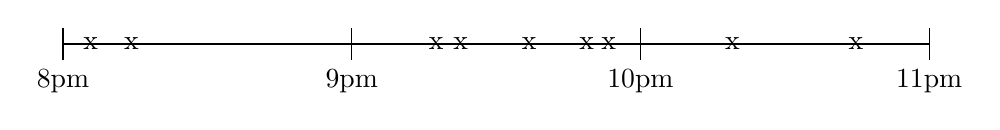
\begin{tikzpicture}

\draw (0,0) -- (11,0)
  node[pos=0.35/11]{x}
  node[pos=0.87/11]{x}
  node[pos=4.74/11]{x}
  node[pos=5.05/11]{x}
  node[pos=5.92/11]{x}
  node[pos=6.65/11]{x}
  node[pos=6.93/11]{x}
  node[pos=8.50/11]{x}
  node[pos=10.07/11]{x}
;
\node[below] at (0,-.2) {8pm};
\draw (0,-.2) -- (0,.2);
\node[below] at (11/3,-.2) {9pm};
\draw (11/3,-.2) -- (11/3,.2);
\node[below] at (22/3,-.2) {10pm};
\draw (22/3,-.2) -- (22/3,.2);
\node[below] at (11,-.2) {11pm};
\draw (11,-.2) -- (11,.2);


\end{tikzpicture}
\end{center}

Let the random variable $Y$ be the number of tweets from
the celebrity in some time interval.
When we say that the number of tweets in a time interval $t$ follows
a Poisson distribution with mean $\lambda t$, we write
\[
  Y \sim \text{Poisson($\lambda t$)}
\]
If $t$ is one hour, then we can write
\[
  Y \sim \text{Poisson($\lambda = 3$)}
\]
Stating that the number of tweets follows a Poisson distribution
implies that the time between tweets follows an Exponential
distribution (and vice versa). Let the random variable $X$ be
the time between tweets. Then
\[
  Y \sim \text{Poisson($\lambda t$)} \Longleftrightarrow X \sim \text{Exp($\lambda$)}
\]
Yes, it is the same $\lambda$ in each distribution.
The average number of tweets is $\lambda=3$ per hour. The average
time between tweets is $1/\lambda = 1/3$ hour (or 20 minutes).
Recall that for the Exponential distribution
\[
  E(X) = \frac{1}{\lambda} = \frac{1~\text{hour}}{3~\text{tweets}} = 20 ~\text{minutes per tweet on average}
\]

Questions.
\begin{enumerate}
\item What is the probability that the celebrity sends out five or
  more tweets in one hour?
\item What is the probability that the celebrity sends out
  no tweets between 9pm and 11pm?
\end{enumerate}

\section{Queueing Models}

\section{Stochastic Dynamic Programming}

\section{Probabilistic Inventory Models}

% first we need to introduce the newsvendor problem.
% perhaps solve this problem as a newsvendor problem.
% also need to make sure that the example of turkeys is OK to use.

\emph{Monte Carlo simulation and Thanksgiving turkeys.}
Tom the grocer pays \$10 wholesale for his turkeys.  Before
Thanksgiving he sells them for \$18.  After Thanksgiving he sells any
remaining turkeys for \$5 each.  In the past years Tom has noticed
pre-Thanksgiving demand has varied uniformly between 50 and 100 birds.
How many turkeys should he buy to maximize his expected profit?

Let's let $x$ represent the number of turkeys that Tom should order.
The random pre-Thanksgiving customer demand is $D$, and Tom's
expect profit is $P$, where

\begin{equation*}
  P = \begin{cases}
    (18 - 10)x & \text{if}~D \geq x \\
    18D - 10x + 5(x - D) & \text{if}~D < x
  \end{cases} 
\end{equation*}
           
Let's find an optimal value for $x$ (our decision variable)
via simulation. Here are the steps.

\begin{compactenum}
\item Set $x = 50,~51,~52,~\ldots,~100$.
  \begin{compactenum}
\item For each value of $x$ generate $B \approx 200$ independent replications
  of $D$, where $D \sim U(50,~100)$. Call the realized values of demand $D_i$ where
  $i = 1 \ldots B$.
\item Calculate the profit $P_i$ for each $D_i$.
  \end{compactenum}
\item Estimate expected profit for each value of $x$ as
  \[ \frac{1}{B} = \sum_{i=1}^B P_i \]
\item Choose the value of $x$ that achieves the maximum profit.
\end{compactenum}

An implementation in R is shown in Figure~\ref{fig:sim-turkeys} and the
output is shown in Figure~\ref{fig:plot-turkeys}.

\begin{SaveVerbatim}{simulation}
Order <- 50:100
EP <- numeric(length(Order))  # will hold expected profit
B <- 200                      # number of replications

for (x in Order) {
    P <- numeric(B)   # will hold realized profits
    for (i in 1:B) {
        D <- sample(50:100, 1)
        if (D >= x) { # sell all turkeys
            P[i] <- 8*x
        } else {      # don't sell them all
            P[i] <- 18*D - 10*x + 5*(x-D)
        }
    }
    EP[which(x==Order)] <- mean(P)
}

plot(Order, EP)   # using base R graphics
\end{SaveVerbatim}

\begin{figure}
\fbox{
\begin{minipage}{\textwidth}
\BUseVerbatim{simulation}
\caption{Simulation to determine the number of turkeys to order
  so that expected profit is maximized.}
\label{fig:sim-turkeys}
\end{minipage}
}
\end{figure}

\begin{figure}
\begin{center}
\includegraphics[width=0.7\columnwidth]{turkeyprofit.pdf}  % change to tikz plot with data
\caption{Plot of expected profit vs. turkeys ordered.}
\label{fig:plot-turkeys}
\end{center}
\end{figure}

\emph{Questions.}
\begin{enumerate}
\item Referring to Figure~\ref{fig:plot-turkeys}, why does it appear
  that the expected profit is becoming more varied as the order
  quantity increases? What can we do about it?
\item Can you solve this problem analytically?
\item Why use simulation?
\end{enumerate}

\emph{Auctioning a turkey.}
On the Wednesday before Thanksgiving, Tom decides to auction a turkey
with the proceeds donated to charity. Tom will offer the turkey using
a second-price sealed-bid auction. In a second-price auction
(also valled a Vickrey auction), the highest bidder wins, but the pays the
price of the second-highest bid.  At the time of the auction it turns
out that there are only two bidders.  Tom doesn't want to give the
turkey away so he sets a reserve price $r$.  The reserve price 
modifies the rules of the auction as follows.  If both bids are below
$r$ then neither bidder wins, and Tom collects no proceeds.
If both bids are at or above $r$ then the regular 2nd-price
auction rules prevail. If only one bid is at or above $r$ then that
bidder wins the turkey and pays $r$. Both bidders agree to the rules.

Now, it is well-known that a 2nd-price is a truth-telling mechanism.
That is to say, bidders will bid their true valuations for the item.
Suppose each bidder has a value for the Turkey is independently and
uniformly distributed between \$0 and \$20.
What is the optimal reserve price $r$?

With some effort, this problem can be solved analytically.
Alternatively, and with not as much effort, we can determine the
optimal reserve price via simulation (see Figure~\ref{fig:auction}.)
Now consider adding just a bit more complexity to the problem, e.g. a
third-price auction, or multiple classes of bidders having different
valuation distributions (Gamma, Lognormal, etc.) The problem can
become intractable to solve analytically, but it is relatively easy to
obtain an approximate optimal solution via simulation.

\begin{SaveVerbatim}{auction}
auction <- function(r) {
    b1 <- runif(1, 0, 20) # bidder 1's valuation
    b2 <- runif(1, 0, 20) # bidder 2's valuation, independent of bidder 1
    if (b1 < r && b2 < r) {
        rev <- 0
    } else if (b1 >= r && b2 >= r) {
        rev <- min(b1,b2) # regular 2nd price auction
    } else {
        rev <- r
    }
    rev
}

reserve <- seq(0, 20, by=.1)
expected.rev <- numeric(length(reserve))

for (i in 1:length(reserve)) {
    expected.rev[i] <- mean(replicate(10000, auction(reserve[i])))
}

plot(reserve, expected.rev, type="l")
\end{SaveVerbatim}

\begin{figure}[h]
\fbox{
\begin{minipage}{\textwidth}
\BUseVerbatim{auction}
\caption{Implementation of a 2nd-price auction with a reserve price $r$ and
  independent valuations for two bidders. We would like to know the reserve
  price $r$ that maximizes revenue for the seller.}
\label{fig:auction}
\end{minipage}
}
\end{figure}


\section{Exercises}

\begin{enumerate}
  
\subsubsection*{Modeling with Probability Distributions.}

% this problem is OK
% geometric distribution
\item \emph{Searching for an item.} Albert has \num{1176} Pok\'{e}mon
  cards in total.  Pok\'{e}mon EX is a special type of card, and
  Albert has 39 EX-type cards.  He is looking for an EX-type card, but
  all of the cards are completely mixed up and stored in a shoe
  box. His mother is calling him for dinner.  What is the probability
  that Albert will have to look through no more than 25 cards before
  he finds an EX-type card?

\begin{solution}
\bs Consider finding an EX-type card to be a ``success''. Let $X$ be a
random variable that represents the number of cards that Albert has to
handle up to and including the first success. Then
\[
X \sim \text{Geometric}(p=\frac{39}{1176})
\]
and
\[
P(X \leq 25) = 1 - (1 - p)^{25} \approx 0.57.
\]
\end{solution}

% this problem is OK
% Binomial, odds, probabilities
\item \emph{Playing Pok\`{e}mon.} Albert is playing
  Pok\'{e}mon cards with his friend. It's Albert's turn, and he
  decides to use Marowak. The card says the following.
\begin{quote}
\emph{Flip a coin four times. The amount of damage done to your opponent's
Pok\'{e}mon is the number of heads times 40.}
\end{quote}
What are the odds that Marowak will do at least 120 damage to the
opponent? One approach to answer this question is to use the Binomial
distribution to compute the probability of doing at least 120 damage
and then convert from probability to odds. You can take another
approach if you prefer. In any case, assume that the coin is fair,
i.e.\ the probability of getting heads on any particular toss is 1/2.

\begin{solution}
\bs
In order to do at least 120 damage, we need either three or four heads
out of the four coin tosses. Let $X$ represent the number of heads obtained
in four tosses of a fair coin. Then $X \sim \text{Binomial}(p=1/2,n=4)$.
\begin{align*}
P(X=3) + P(X=4) &= {4 \choose 3} p^3 (1-p)^1 + {4 \choose 4} p^4 (1-p)^0 \\
&= \frac{1}{4} + \frac{1}{16} \\
&= \frac{5}{16}
\end{align*}
The odds are
\[
\frac{p}{1-p} = \frac{\frac{5}{16}}{1-\frac{5}{16}} = \frac{5}{11}
\]
or 5 to 11.
\end{solution}

% binomial distribution
\item \emph{System reliability.}  A data warehouse has $n$ servers.
Each server will fail, independently, with probability $p$.
\begin{enumerate}
\item Suppose that a single functioning server can support the
  integrity of the data. What is the probability that data will be
  lost? \label{ex:p1}
\item Suppose that two functioning servers are required for data
  integrity.  What is the probability that data will be lost?
\label{ex:p2}
\end{enumerate}

\begin{solution}
  \bs For part~\ref{ex:p1}, all $n$ servers must fail for data to be
  lost.  Because failures are independent, the probability of data
  loss due to server failure is $p^n$.

For part~\ref{ex:p2}, let $X$ be the number of failed servers. $X$
has a Binomial distribution with parameters $n$ and $p$. The probability
of data loss due to server failure is
\begin{align*}
      P(X \geq n-1) &= \sum_{i=n-1}^n {n \choose i} p^i (1-p)^{n-i} \\
      &= {n \choose n-1} p^{n-1} (1-p)^{n-(n-1)} + {n \choose n} p^n (1-p)^{n-n} \\
      &= np^{n-1}(1-p) + p^n \\
      &= np^{n-1} - np^{n-1}p + p^n\\
      &= np^{n-1} - np^n + p^n\\
      &= np^{n-1} + (1-n)p^n
\end{align*}
\end{solution}

% this problem is OK
% exponential distribution
\item \emph{Evaluating a warranty.}
  A manufacturer of automotive batteries offers a one-year
  warranty. If the battery fails for any reason during the warranty
  period, it is replaced for free. The time to failure is distributed
  Exponential with rate $\lambda=.125$ failures per year.
\begin{enumerate}
\item What proportion of batteries fail within the warranty period?
\item The cost to manufacture a battery is \$50, and the profit
per battery is \$25. What is the effect of the warranty replacement
policy on profit? \label{ex:profit}
\end{enumerate}

\begin{solution}
  \bs The question is asking for the theoretical proportion of
  batteries that fail within one year. Since all batteries have the
  same probability of failure, this proportion is equal to the
  probability that a single battery will fail within one year. Let $X$
  be a random variable that represents the time to failure.
\[ P(X<1) = 1-e^{-\lambda t} = 1 - e^{-.125} = 0.118 \]
Now, imagine that the manufacturer has, over time,
  sold many batteries and has kept data on how many batteries failed
  within one year. The empirical proportion is simply the number
  of batteries that failed divided by the number of batteries sold.
  The Law of Large Numbers tells us that when the number of batteries
  sold is large, the empirical proportion will be approximately
  equal to the theoretical proportion.

Taking the warranty into account, the average profit per battery is
\[ \$25 - 0.118\times \$50 = \$19.10 \]
So, the (average) effect of the warranty on profit is -\$5.90.
\end{solution}

% memoryless property of the Exponential distribution this problem is
% from Ross. It's a thought experiment. The actual numbers don't
% matter as long as the rates are the same. Can we find a different
% scenario that illustrates the same idea: the memoryless property
\item \emph{Memoryless property of the Exponential distribution.} A
  hair salon has two hairdressers who provide haircuts on a walk-in
  basis. Sam arrives to the salon and finds that both hairdressers are
  busy with customers. However, no other customers are waiting, so Sam
  will begin his haircut (immediately) when the first space opens up.
  Suppose that the distribution of service times for both hairdressers is
  exponential with rate $\lambda$. What is the probability that
  Sam is the last of the three customers to complete a haircut?

\begin{solution}
  \bs By the memoryless property of the Exponential distribution, the
  distribution of remaining time for each customer currently receiving
  a haircut is exponential with rate $\lambda$.  Since the two
  customers getting haircuts have the same distribution for remaining
  time, the probability that customer 1 finishes before customer 2 is
  1/2 (likewise for customer 2 finishing before customer 1). When Sam
  enters service, the memoryless property still applies.  Regardless
  of how long the other customers have been in service, Sam has the
  same distribution for remaining time. The probability Sam is the
  last to finish is 1/2.
\end{solution}

% Poisson distribution
\item \emph{Donut giveaway.}  A professional baseball team has just
  won a game that secured them a berth in the league’s playoffs. To
  celebrate, a local donut shop will be giving away up to 200 free
  donuts during a two-hour period on the morning following the
  victory. All 200 donuts will be baked and decorated with a baseball
  theme before the giveaway starts. If there are any donuts remaining
  after the giveaway, they will be sold at a discounted price. Assume
  that customers will arrive at the giveaway according to a Poisson
  process at a mean rate of 100 customers per hour. Also, note that
  there is a limit of one donut per customer.
\begin{enumerate}
\item What is the probability that there will be donuts remaining
  after the giveaway? \label{ex:donuta}
\item What is the predicted number of donuts that will be remaining
  after the giveaway? \label{ex:donutb}
\end{enumerate}

For part~\ref{ex:donuta}, present your answer as an expression for the
probability that there will be donuts remaining. Then, use software,
such as R, to compute a numerical answer.

\begin{solution}
  \bs Given that customers arrive to the giveaway according to a
  Poisson process with a mean of 100 customers per hour, the number of
  customers that arrive during the two-hour period is Poisson
  distributed with a mean of 200. Let $N$ be the number of customers
  arriving in a two-hour period. Then
  \[ N \sim \text{Poisson}(\lambda = 200) \] 
For part~\ref{ex:donuta},
  the probability that there will be donuts remaining after the
  giveaway is
\begin{align*}
P(N < 200) &= \sum_{n=0}^{199} \frac{\lambda^n e^{-\lambda}}{n!}\\
&= \sum_{n=0}^{199} \frac{200^n e^{-200}}{n!}\\
&\approx .49
\end{align*}
In R,
\begin{Verbatim}
> sum(dpois(0:199,200))
[1] 0.4905966
\end{Verbatim}  

For part~\ref{ex:donutb}, our calculations are all done in expectation
(that is to say, on average). There are 200 customers in 2 hours,
which means that 200 donuts are given away. So, on average, no donuts
remain.
\end{solution}

% re-written by hannah
% Poisson distribution
\item \emph{Startup expenses.}  Two friends are starting a small
  business selling ice cream. They applied for a grant and have
  received \$\num{1800} to help cover any startup expenses. The
  friends will incur expenses of \$300 randomly throughout the first
  year, and the time between payments for these expenses is
  exponential with a mean of 2 months. Determine the probability that
  the friends will run out of grant money before the end of the year.

\begin{solution}
  \bs Let $X$ be a random variable that represents the time between
  payments. The mean time between payments, that is to say the
  expected value of $X$ ($E(X)$), is two months. We know that for the
  Exponential distribution
  \[ E(X) = \frac{1}{\lambda} \] where $\lambda$ is the rate (in units
  of payments per month). So,
  \[ X \sim \text{Exp}(\lambda = 1/2~\text{payments per month}) \] If
  the time between payments is distributed Exponential with rate
  $\lambda$, then the number of payments in $t$ months is Poisson with
  mean $\lambda t$. Let $N$ be the number of payments in 12 months.
  \[ N \sim \text{Poisson}(\lambda t = \lambda \times 12 = 6) \] Now,
  the probability that the friends runs out of money is
\begin{align*}
      P(N \geq 6) &= 1 - P(N \leq 5) \\
      &= 1 - \sum_{n=0}^{5} \frac{\lambda^n e^{-\lambda}}{n!}\\
      &= 0.55
\end{align*}
You may have defined the event that the friends runs out of
money as $P(N = 6)$. In other words, that there are exactly
six payments during the first year.  This is incorrect because
we are modeling the spending activity as a Poisson process. In
other words, the (unstated) assumption is that the number of
payments is independent of the available funds.
\end{solution}

% re-written by hannah
% poisson distribution
\item \emph{Stocking a vending machine.}  A university cafeteria has a
  vending machine that is stocked with a variety of juices and
  sodas. A student employee replenishes inventory weekly so that there
  are 180 beverages in stock at the beginning of each week. The
  cafeteria is open 24 hours, 7 days a week, and beverages are
  purchased according to a Poisson process with a mean of 1 hour
  between purchases.
\begin{enumerate}
\item What is the probability that, at the end of any given week, the
  student employee will find the machine to be sold out? \label{ex:pout}
\item On average, how many beverages remain in the vending
  machine when the employee arrives? \label{ex:qremain}
\item What is the probability that the employee will replenish 150 or
  more beverages? \label{ex:preplenish}
\end{enumerate}

\begin{solution}
  \bs For part~\ref{ex:pout}, there will be no beverages remaining in
  the vending machine if demand for beverages is at least 180.
  Because the beverages are purchased according to a Poisson
  process with a mean of one hour between purchases, the rate
  $\lambda$ that beverages are purchased is 24 beverages per
  day. This means that the number of purchases in seven days is Poisson
  with mean $\lambda t$. Let $N$ be a random variable that represents
  the number of purchases in one week (seven days).
  \[ N \sim \text{Poisson}(\lambda = \lambda \times 7 = 168) \] 
\begin{align*}
      P(N \geq 180) &= 1 - P(N \leq 179)\\
      &= 1 - \sum_{i=0}^{179} \frac{168^i e^{-168}}{i!}\\
      &\approx 0.19
\end{align*}
In R,
\begin{Verbatim}
> 1 - sum(dpois(0:179,168))
[1] 0.1866995
\end{Verbatim}

For part~\ref{ex:qremain}, the expected number of beverages purchased
from the vending machine each week is 168. The expected number of
beverages remaining at the end of the week is $180-168=12$.
	
For part~\ref{ex:preplenish}, The probability that 150 or more
beverages are purchased during a week is
\begin{align*}
      P(N \geq 150) &= 1 - P(N \leq 149)\\
      &= 1 - \sum_{i=0}^{149} \frac{168^i e^{-168}}{i!}\\
      &\approx 0.93
\end{align*}
In R,
\begin{Verbatim}
> 1 - sum(dpois(0:149,168))
[1] 0.9253016
\end{Verbatim}
\end{solution}

% re-written by hannah
% Poisson distribution
\item \emph{Car dealership.} A used car dealership parks their
  inventory on an uncovered lot. In the city where the dealership is
  located, the probability of a hailstorm during the month of June is
  0.30. If a hailstorm occurs, the number of dents in a randomly
  chosen car follows a Poisson distribution with a mean of five dents.
\begin{enumerate}
\item If a car receives no more than one dent during a hailstorm,
the dealership ignores it and hopes that the customer will not notice.
Given that a hailstorm occurred, compute the probability that a car
receives no more than one dent.~\label{ex:dent}
\item The occurrence of a storm and the amount of damage after a storm
  are independent. (Of course damage is conditional on the occurrence
  of a storm.)  If a car has more than five dents after a storm, then
  the dealership must file an insurance claim for the car. It is May 31
  and there are 100 cars on the lot. Determine the expected number of
  cars for which the dealership will file insurance during June
  (assume that the inventory remains constant at 100
  cars).\label{ex:cars}
\end{enumerate}

\begin{solution}
  \bs For part~\ref{ex:dent}, let $N$ be a random variable that
  represents the number of dents in a car after a hailstorm.  We know
  that
 \[ N \sim \text{Poisson}(\lambda = 5). \]
  The probability that a car receives no more than one dent is
\begin{align*}
P(N \leq 1) &= P(N=0)+P(N=1) \\
&= \frac{e^{-\lambda}\lambda^0}{0!} + \frac{e^{-\lambda}\lambda^1}{1!} \\
&\approx 0.04
\end{align*}

Conditional on the occurrence of a hailstorm, the probability that any
particular car receives more than 5 dents is
\begin{align*} P(N \geq 6) &= 1-P(N\leq 5) \\
&= \sum_{i=0}^5 \frac{e^{-\lambda}\lambda^i}{i!}\\
&\approx 0.384,
\end{align*}
and the (unconditional) expected number of such cars is
\[ 0.30 \times P(N \geq 6) \times 100 \approx 11.5 \]
Using R, 
\begin{Verbatim}
> 0.30 * (1 - sum(dpois(0:5,5))) * 100
[1] 11.52118
\end{Verbatim}
\end{solution}

% this problem is OK
% a poisson process, memory-less property of exponential distribution
\item \emph{A mining operation.} A dump truck at a mine takes ore to
  the railroad after 10 one-ton scoops have been loaded into the
  truck.  The one-ton scoops are loaded from a large diesel-powered
  shovel at a mean rate of seven scoops per hour.  The time between
  scoops from the shovel follows an Exponential distribution.

\begin{enumerate}
\item Find the probability that the time required to load the truck
takes at least one hour.
\item It takes the dump truck 18 minutes to travel to the railroad,
  unload, and return. Suppose the truck returns and finds that no
  scoop is waiting to be loaded. What is the probability that the next
  scoop is ready within 5 minutes? \label{item:2}
\end{enumerate}

\begin{solution}
  \bs The time between scoop arrivals is distributed Exponential, so
  we know that the number of arrivals in a time interval is
  distributed Poisson. In particular, the number of arrivals in a
  one-hour period follows a Poisson distribution with mean
  $\lambda=7$. In order for the time required to load the truck be at
  least one hour, the number of scoops in one hour be nine or
  less. Let $N$ be the number of scoops in a one hour period.
\[
P(N \leq 9) = \sum_{x=0}^9 \frac{e^{-\lambda}\lambda^x}{x!} = .83.
\]
For part \ref{item:2}, we can invoke the memoryless property of the
Exponential distribution. The remaining time until the next arrival is
disitributed Exponential with rate 7 scoops per hour, regardless of
how much time has elapsed since the last arrival. Let $Y$ be the
remaining time until the next arrival, and don't forget to convert
from minutes to hours.
\[
P(Y \leq 5) = 1 - e^{-7\times \frac{5}{60}} = .44
\]
\end{solution}

% re-written by hannah
% normal distribution
\item \emph{Blood pressure screening.} High blood pressure is an
  underlying health condition that makes people more susceptible to
  severe illness. A company conducted blood pressure screenings to
  determine the risk its employees have for severe illness. The
  systolic blood pressures (SBP) of 220 employees were measured.  In
  the general population, SBP measurements follow a Normal distribution
  with mean $\mu=135$ and with standard deviation $\sigma=20$.  The
  company doctor has created the following guidelines for determining
  which employees are at highest risk.

\begin{tabular}{rl}
	systolic blood pressure & risk \\ \hline
	$\mu+1.5\sigma < SBP$ & very high \\
	$\mu < SPB \leq \mu+1.5\sigma$ & high \\
	$\mu-\sigma < SBP \leq \mu$ & average \\
	$SBP \leq \mu-\sigma$ & low
\end{tabular}

How many employees of this company fall into each of the four categories?

\vspace{.1in}
\begin{solution}
\bs Let $X \sim \mathcal{N}(\mu=135,~\sigma=20)$ be a random variable that represents
systolic blood pressure, and recall that $\Phi(z)$ indicates the CDF of the
standard Normal distribution.
\begin{align*}
\text{very high}&
\quad 220\times(1-P(X \leq \mu+1.5\sigma))=220\times(1-\Phi(1.5)) \approx 15 \\
\text{high}&
\quad 220\times (P(X \leq \mu+1.5\sigma)-P(X \leq \mu))=220\times(\Phi(1.5)-\Phi(0)) \approx 95 \\
\text{average}&
\quad 220\times(P(X \leq \mu)-P(X \leq \mu-\sigma))=220\times(\Phi(0)-\Phi(-1))\approx 75 \\
\text{low}&
\quad 220\times(P(X \leq \mu-\sigma))=220\times\Phi(-1) \approx 35
\end{align*}
\end{solution}

% this problem is OK
% Lognormal distribution
\item \emph{Time to failure.} The lifetimes of parts or components
  that are subjected to the environment (i.e. temperature, corrosion,
  stress, chemicals) are often modeled using a Lognormal
  distribution. Rather than being additive, the environmental factors
  that influence the time to failure are multiplicative. The Central
  Limit Theorem applies, but because the random effects are
  multiplicative on the time scale, they are additive on the log
  scale.  

  A certain component of a bridge is inspected annually to see if it
  needs to be replaced. The lifetime of the part follows a Lognormal
  distribution with parameters $\mu=1.6$ and $\sigma=0.25$.

\begin{enumerate}
\item Determine the mean time to failure for this part.
\item What is the probability that the part will last longer
than seven years?
\end{enumerate}

\begin{solution}
  \bs Let $X$ be a random variable that represents the time to failure
of a part. Then  
\[ X \sim \text{LogN}(\mu=1.6,\sigma=0.25). \]
The mean time to failure is
\[ e^{\mu + \sigma^2/2} \approx 5.1~\text{years.} \]

We wish to find $P(X > 7)$. Taking logarithms and standardizing,
\begin{align*}
      P(X > 7) &= P(\ln(X) > \ln(7)) \\
      &= P\left(Z > \frac{\ln(7)-1.6}{0.25}\right) \\
      &= P(Z > 1.38) \\
      &= 1-P(Z \leq 1.38) \\
      &= 0.084
\end{align*}

\end{solution}


\subsubsection*{Stochastic Processes}

\subsubsection*{Queueing Models}

% this problem is ok.
\item \emph{Performance metrics for a queueing system.} Consider a
  single server queueing system with FIFO queue discipline.  For the
  particular day that this system was in operation, the arrival times
  and the service times of the first six customers were
  (0,3,7,9,10,12) and (4,6,2,1,3,1), respectively. Arrival times and
  service times are in minutes.  Compute the average waiting time and
  the average number of customers in the queue for the first six
  customers. It will help to construct a diagram of number in
  system versus time.

\begin{solution}
\bs
    
\pgfplotsset{compat=1.12}
\begin{center}
  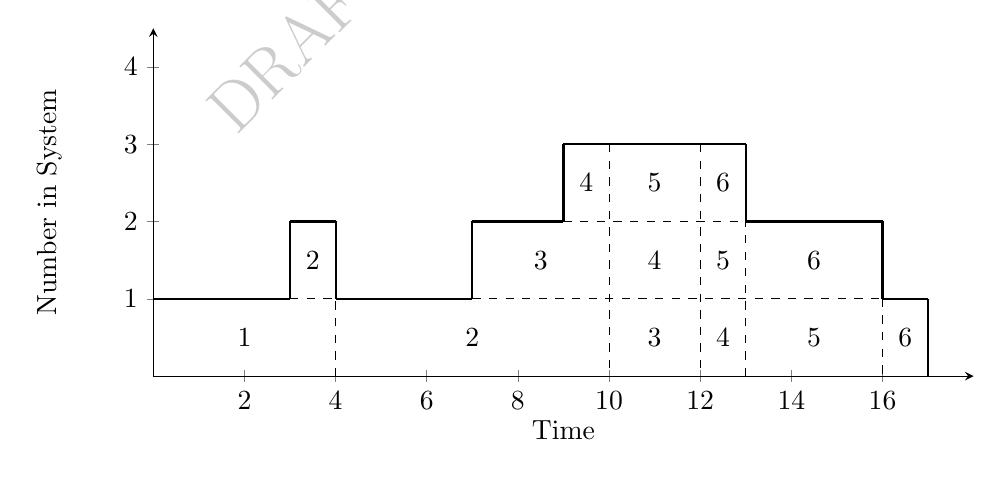
\begin{tikzpicture}[scale=1.0]
    \begin{axis}[clip=false,
      width=12cm, height=6cm,
    axis x line=middle,
    axis y line=middle,
    ymin=0, ymax=4.5,
    ytick={0,1,2,3,4},
    yticklabels={0,1,2,3,4},
    xmin=0, xmax=18,
    xtick={2,4,6,8,10,12,14,16},
    xticklabels={2,4,6,8,10,12,14,16},
    x label style={at={(axis description cs:0.5,-0.1)},anchor=north},
    y label style={at={(axis description cs:-0.1,.5)},rotate=90,anchor=south},
    xlabel=Time,
    ylabel=Number in System,
    ]
    \addplot[mark=none, style=thick] coordinates { (0, 1) (3, 1) };
    \addplot[mark=none, style=thick] coordinates { (3, 1) (3, 2) };
    \addplot[mark=none, style=thick] coordinates { (3, 2) (4, 2) };
    \addplot[mark=none, style=thick] coordinates { (4, 1) (4, 2) };
    \addplot[mark=none, style=thick] coordinates { (4, 1) (7, 1) };
    \addplot[mark=none, style=thick] coordinates { (7, 1) (7, 2) };
    \addplot[mark=none, style=thick] coordinates { (7, 2) (9, 2) };
    \addplot[mark=none, style=thick] coordinates { (9, 2) (9, 3) };
    \addplot[mark=none, style=thick] coordinates { (9, 3) (13,3) };
    \addplot[mark=none, style=thick] coordinates { (13, 3) (13,2) };
    \addplot[mark=none, style=thick] coordinates { (13,2) (16,2) };
    \addplot[mark=none, style=thick] coordinates { (16,2) (16,1) };
    \addplot[mark=none, style=thick] coordinates { (16,1) (17,1) };
    \addplot[mark=none, style=thick] coordinates { (17,1) (17,0) };

    \addplot[mark=none,dashed] coordinates { (3,1) (4,1) };
    \addplot[mark=none,dashed] coordinates { (7,1) (16,1) };
    \addplot[mark=none,dashed] coordinates { (9,2) (13,2) };
    \addplot[mark=none,dashed] coordinates { (10,3) (10,0) };
    \addplot[mark=none,dashed] coordinates { (12,3) (12,0) };
    \addplot[mark=none,dashed] coordinates { (16,1) (16,0) };
    \addplot[mark=none,dashed] coordinates { (4,0) (4,1) };
    \addplot[mark=none,dashed] coordinates { (13,0) (13,2) };

    \node at (2,.5) {1};
    \node at (3.5,1.5) {2};
    \node at (8.5,1.5) {3};
    \node at (9.5,2.5) {4};
    \node at (7,.5) {2};
    \node at (11,.5) {3};
    \node at (11,1.5) {4};
    \node at (11,2.5) {5};
    \node at (12.5,.5) {4};
    \node at (12.5,1.5) {5};
    \node at (12.5,2.5) {6};
    \node at (16.5,.5) {6};
    \node at (14.5,.5) {5};
    \node at (14.5,1.5) {6};

  \end{axis}
\end{tikzpicture}
\end{center}

First note that the problem description does \emph{not} tell us that
the times between arrivals and/or the service times are exponentially
distributed. So it is not an $M/M/1$ system.
The total delay of all six customers is $0+1+3+3+3+4=14$. The average
waiting time in the queue is the total delay divided by the number
of customers.
\[ W_q = \frac{14}{6} = 2.3333~\text{min} \]
To compute the average number in the queue, weight the time in queue
by the number of customers. In other words, compute the area under the
curve but above one, and then divide by the total time.
\[ L_q = \frac{14}{17} \]
\end{solution}

% re-written by hannah.
\item \emph{Justification for a capital expense.} An amusement park is
  known for having rides with short waiting times. A new ride has
  opened, and customers arrive to the ride according to a Poisson
  process with a mean of 20 arrivals per hour. Only one customer is
  allowed on the ride at a time, and customers can stay on the ride as
  long they wish. The length of time that each customer spends on the
  ride is exponentially distributed with a mean of 2.5
  minutes. Management is willing to add an additional cart to the ride
  if, under the current system, 1) the average number of waiting
  customers is greater than four, and 2) the percentage of time that
  the ride is idle exceeds 10\%.  Can an additional cart be justified?

\begin{solution}
  \bs The amusement ride can be modeled as an M/M/1 queuing
  system. Customers arrive at the rate
\[ \lambda = 20~\text{customers per hour,} \]
and the service rate is 
\[ \mu = 24~\text{customers per hour.} \]
To see whether the first condition is satisfied, we compute
\[ L_q = \frac{\lambda^2}{\mu(\mu-\lambda)} = \frac{20^2}{24(24-20)} =
  25/6 > 3~\text{customers} \] 
and so the first condition is satisfied. To
see if the second condition is satisfied, we compute
\[ p_0 = 1 - \frac{\lambda}{\mu} = 0.167 \]
and so the second condition is also satisfied.
\end{solution}

% re-written be hannah
\item \emph{Comparing system configurations.}  Patients arrive to an
  emergency room according to a Poisson process at the rate of 10
  patients per hour. Before a patient can see a doctor, they must have
  their medical history reviewed and their vitals measured. Currently,
  the hospital has one nurse who performs both of these tasks for each
  patient. The time that each patient spends with the nurse is
  exponentially distributed with a mean of five minutes. An Industrial
  Engineer at the hospital is considering two options for improving
  service.
\begin{compactenum}
\item Hire a medical scribe to review each patient's medical history
  while the nurse takes vitals. The service rate would increase to 20
  patients per hour with this improved single-server operation
(service times are still exponentially distributed.) \label{ex:scribe}
\item Hire a second nurse who also reviews medical history and takes
  vitals for each patient. The two nurses would each have a service
  rate of 12 patients per hour (each with exponential service times)
  with this two-server operation.
\end{compactenum}
Consider the relative cost of each option and evaluate the
improvements that would result. Then, determine which option the
engineer should recommend.

\begin{solution}
  \bs We will look at the average number of patients in the queue
  $L_Q$ and the average time in queue $W_Q$ as metrics to judge
  improvement in system performance. Before any improvements are made,
\[ L_q = \frac{\lambda^2}{\mu(\mu-\lambda)} = \frac{10^2}{12(12-10)} = 25/6 = 4.167~\text{patients} \]
and
\[W_q = \frac{L_q}{\lambda} = \frac{25/6}{10} = 5/12~\text{hours} = 25~\text{minutes} \]
If they hire a scribe to assist the nurse
\[ L_q = \frac{\lambda^2}{\mu(\mu-\lambda)} = \frac{10^2}{20(20-10)} = 0.5~\text{patients} \]
and
\[W_q = \frac{L_q}{\lambda} = \frac{0.5}{10} = 0.05~\text{hours} =
  3~\text{minutes} \] 
and if they add an additional nurse we need to
use the formulas for a two-server operation. First,
\[ P_0 = \frac{1}{\sum_{n=0}^{k-1}\frac{\left(\lambda/\mu\right)^n}{n!} + \frac{\left(\lambda/\mu\right)^k}{k!}\left(\frac{k\mu}{k\mu-\lambda}\right)} \]
where $k=2$ servers. Then
\[ L_q = \frac{\left(\lambda/\mu\right)^k\lambda\mu}{(k-1)!(k\mu-\lambda)^2}P_0 \]
and
\[W_q = \frac{L_q}{\lambda} \] 
Plugging values, I got $P_0=0.4118$,
$L_q=0.1751$ patients, and $W_q=0.0175$ hours or $1.05$ minutes.
Considering the relative improvement and the cost of adding a second
nurse, I would recommend option~\ref{ex:scribe}. That is, to hire a scribe to help
the nurse. The average number in queue and the average time in queue
appear to be acceptable for an emergency room setting.
\end{solution}

% the context of this problem needs to be re-written. perhaps describe a
% situation of a store with two clerks, each with exponential service times
% (so total service time is Gamma/Erlang). Social distancing measures mean
% that only one customer at a time is allowed in the store.
\item \emph{An $M$/$G$/$1$ queue.}  A coffee shop has recently opened
  for takeout after being closed due to COVID-19. In order to follow
  public health guidelines, only one customer is allowed in the shop
  at a time. If a customer is being served, any customer
  that arrives must wait in a line outside of the coffee
  shop. Customers arrive at a rate of 12 customers per hour, and
  inter-arrival times are exponentially distributed. The shop has two
  baristas: one barista takes orders and the other prepares the
  beverages. The service time for each barista to complete their task
  is independently and exponentially distributed with a mean of two
  minutes. Determine the average number of customers waiting in line
  to be served, $L_Q$. A couple of helpful items:
\begin{compactenum}[i)]
\item The variance of the sum of independent
random variables is the sum of the variances,
\item the sum of IID
exponential random variables is distributed Gamma, 
\item the variance
of an exponential distribution is the mean squared, and
\item for an $M$/$G$/1 queue, 
\[ L_Q = \frac{\rho^2(1 + \sigma^2\mu^2)}{2(1-\rho)} \]
where $\rho$ is the server utilization, $\mu$ is the service rate, and $\sigma^2$ is
the variance of the service time distribution.
\end{compactenum}

\begin{solution}
\bs The first thing to note is that the service time is the sum of two IID exponential
random variables, and so we know that it has a Gamma distribution.
Letting $X$ represent the service time,
\[ \text{Var}(X) = 2^2 + 2^2 = 8.\]
The expected total service time for both baristas is 4 minutes, so
$\mu = 1/4$ customers per minute. 
Now, in units of customers per minute, the arrival rate is $\lambda = 1/5$.
\begin{align*}
      L_Q &= \frac{\frac{16}{25}\left(1 + 8\left(\frac{1}{16}\right)\right)}{2\left(\frac{1}{5}\right)} \\
      &= 2.4 ~\text{customers}
\end{align*}
\end{solution}


\subsubsection*{Stochastic Dynamic Programming}

\subsubsection*{Probabilistic Inventory Models}

% written by Emily
% Probabilistic Inventory Model

\item \emph{Stocking a seasonal item.} Summer is approaching and a
  store is determining how many folding lawn chairs they should
  purchase from a supplier.  Each chair costs \$15\ for the store to
  purchase and can be sold for \$27.50.\ The store stocks lawn chairs
  only during the summer; any chairs left at the end of the summer are
  sold at a clearance price of \$10.50.\ Based on historical data, the
  seasonal summer demand for lawn chairs follows a normal distribution with
  $\mu = 205$ and $\sigma = 25$.

\begin{enumerate}
\item What is your recommended order quantity for the store?
\item What is the probability that the store will sell all the folding
  lawn chairs it orders before summer is over? \label{ex:lawn}
\item How would the economic order quantity change if the clearance
  price for the chairs was only \$8?\ What happens to the store's
  order quantity as the clearance price is reduced? \label{ex:clearance}
\end{enumerate}

\begin{solution}
  \bs Let $D$ be the summer demand for folding lawn chairs. We know
  that $D \sim \mathcal{N}\left(\mu=205,~\sigma=25\right)$. The
  penalty for ordering too few items is $c_u= 12.50$ and the penalty
  for ordering too many items is $c_o= 4.50$. We want to find the
  order quantity $Q^{\ast}$ such that


\[ P\left(D \leq Q^{\ast}\right) < \frac{c_u}{c_u+c_o} = \frac{12.50}{17.00} = 0.735 \]
Standardizing,
\[ P\left(z \leq \frac{Q^{\ast}-205}{25}\right) = 0.735 \]
implies that
\begin{align*}
\frac{Q^{\ast}-205}{25} &= 0.63 \\
Q^{\ast} &= 205 + 0.63(25)\\
Q^{\ast} &= 220.75
\end{align*}

The store should order 221 (or 220) folding lawn chairs. 
If we are using R, we can obtain the answer without standardizing
by simply passing the mean and standard deviation to \texttt{qnorm},
\begin{Verbatim}
> qnorm(.735, 205, 25)
[1] 220.7002
\end{Verbatim}

For part~\ref{ex:lawn}, the probability that all chairs will sell is


\begin{align*}
  P\left(D \geq 221 \right) &= 1 - P\left(D \leq 221 \right)\\
                            &= 1 - P\left( z \leq \frac{221-205}{25} \right) \\
                            &= 1 - P\left( z \leq .64 \right)\\
                            &= 1 - .74 \\
                            &= 0.26
\end{align*}


Regarding part~\ref{ex:clearance}, if the clearance price decreases to
\$8\, then the cost of being under-stocked will still be $c_u=12.50$,
but the cost of being over will increase to $c_o=7.00$. The order
quantity $Q^{\ast}$ will change such that

\begin{align*}
  P\left(D \leq Q^{\ast}\right) = \frac{12.50}{19.50} &= .641 \\
  P\left(z \leq \frac{Q^{\ast}-205}{25}\right) &= .641
\end{align*}
which implies that
\begin{align*}
  \frac{Q^{\ast}- 205}{25} &= .36\\
  Q^{\ast} &= 205 + 0.36(25) = 214
\end{align*}

With a clearance price of \$8, the new order quantity will be 214
chairs.  The economic order quantity will continue to decrease as the
clearance price decreases because the cost of being over will continue
to increase.
\end{solution}

% written by Emily
% Uniform distribution
\item \emph{Programs for sale.}  A college hockey team has game
  programs for sale at every home game they play. The demand $D$ for
  these programs is a random variable that follows a Uniform
  distribution with a minimum of \num{1200} programs and a maximum of
  \num{2000} programs.
  \[ D \sim \text{Uniform}(1200,\,2000) \] Each program costs \$1\ to
  produce and sells for \$3.\ The programs contain information
  specific to the game, so any unsold programs are thrown away after
  the game. How many game programs should the college print per game
  to maximize their revenue? You should use the CDF of the Uniform
  distribution to answer this question.
  
\begin{solution}
\bs 
The CDF of Uniform distribution is
\[ P(X \leq x) = F(x) = \int_{y=a}^x f(y)\,dy = \int_{y=a}^x
  \frac{1}{b-a}\,dy = \frac{x-a}{b-a} \] for $a \leq x \leq b$.  The
cost per copy of being over/under is $c_o = \$1$ and $c_u = \$2$,
respectively.  Let $Q^{\ast}$ be the optimal number of copies to
produce.  Using the critical ratio, we want
\[ P\left(D \leq Q^{\ast}\right) = \frac{c_u}{c_u+c_o} = 
\frac{2}{3} \approx 0.667 \]
Using the definition of the CDF for the Uniform distribution,
\begin{align*}
  \frac{Q^{\ast} - 1200}{2000-1200} &= 0.667 \\
    Q^{\ast} &= 0.667\times 800 + 1200\\
    Q^{\ast} &= 1734
\end{align*}
The college should print 1734 copies.
\end{solution}

% written by Emily
\item \emph{The risk of being out-of-stock.}
The daily demand for milk cartons in a school cafeteria
follows a Normal distribution with mean 600 and standard
deviation 20. It costs \$.01 per day to hold one item in
inventory. The fixed cost to make a replenishment order is
\$50, and the lead time to receive an order is 2 days.

\begin{enumerate}
\item Currently, the inventory policy for milk cartons is 
to order \num{3000} cartons whenever the inventory drops 
to \num{1225} units. Determine the probability of a 
stock-out under this policy. \label{ex:pol}

\item Running out of milk generates lots of complaints to the
PTA. Recommend an inventory policy for the school when
the probability of a stock-out cannot exceed .01.
Your policy should include an economic order quantity and 
a re-order point.
\label{ex:so-policy}

\item Compare the cost of the policy in part~\ref{ex:pol} with 
the cost of the policy in part~\ref{ex:so-policy}. \label{ex:comp-pol}
\end{enumerate}

\begin{solution}
\bs The distribution of demand during lead time $X_m$ is
\[ X_m \sim \text{Normal}(\mu_m=1200,\sigma_m=\sqrt{800}) \]
The probability of a stock-out is
\begin{align*}
  P(X_m \geq 1225) &= P\left(z \geq \frac{1225-\mu_m}{\sigma_m}\right) \\
                  &= 1 - P\left(z < \frac{1225-1200}{\sqrt{800}}\right) \\
                  &= 1 - P\left(z < 0.8839\right) \\
                  &= 1 - .8106 \\
                  &\approx .19
\end{align*}

With the requirement that the probability of a stock-out not exceed
0.01, the optimal order quantity is
\[
  Q^{\ast} = \sqrt{\frac{2C_oD}{C_h}} = 
  \sqrt{\frac{2\times 50\times 600}{.01}} \approx 2450
\]
Without a buffer stock the optimal policy is to order 
\num{2400} milk cartons every $T_0=Q^{\ast}/D \approx 4$ days. 
To compute the buffer stock, we want
\[
  P(X_m \geq B + 1200) \leq 0.01
\]
or equivalently, we want $B \geq \sigma_m \times 
2.33 \approx 66$.
The best policy is to order \num{2400} milk cartons 
whenever the inventory drops to $\num{1200}+66=\num{1266}$ units.

On average, the total daily cost of the current inventory policy (not
considering the frustration costs of a stock-out) consists of the
holding cost and the ordering cost. The holding cost has two terms:
one for the normal inventory and one for the buffer stock
\begin{align*}
 & \left(\frac{Q}{2}\right)\left(C_h\right)  + \left(25\right)\left(C_h)\right)\\
= & \left(\frac{3000}{2}\right)\left(0.01\right) + (25)(0.01) \\
= & \$15 + \$0.25 \\
= & \$15.25 ~\text{per day.}
\end{align*}
The ordering cost of the current policy is
\[ \left(\frac{600}{3000}\right) \left(50\right) = \$10~\text{per
    day.} \] Remember that demand is random and so these costs are
``on average''.  The only difference in cost for the new inventory
policy in part~\ref{ex:so-policy} is the increased holding cost for
the larger buffer stock. This amounts to an increase of
\[ (66 - 25) (0.01) = \$0.41~\text{per day.} \]
Assuming the milk does not expire before it is used, the benefit
of fewer stock-outs seems to be worth the increase in cost.
\end{solution}

\end{enumerate}
%%% Local Variables:
%%% TeX-master: "main"
%%% End:

\chapter{Decision Problems}

\section{Games Against Nature}

% also we need a section on using backward induction to solve
% decisions over time. relate it to DP.

\section{Games Against an Opponent}

% this will be the last portion of this section, where we bring together
% several concepts. Need to re-write this section: change the context
% of the problem and explain the methodology.
\emph{Nature as an adversary: a two-person zero-sum game.}
Merrill has a concession stand at Target Field for the sale of
sunglasses and umbrellas. This entrepreneur likes to make sales
regardless of the weather.  When it rains can sell about 500
umbrellas.  On a sunny day he can sell about 100 umbrellas and about
1000 sunglasses. Umbrellas cost him 50 cents and sell for \$1.
Sunglasses cost him 20 cents each and sell for 50 cents. Merrill is
willing to invest \$250 in the concession stand business.  All unsold
items represent a loss; there is no salvage value. 

Formulate Merrill's problem as a two-person zero--sum game. Merrill is
the row player and Nature is the column player. Merrill's strategy set
is \{buy inventory for rain, buy inventory for sun\}. Nature's strategy
set is \{rain, sun\}. The payoff entries represent the profit/loss.
Find an equilibrium strategy for Merrill. That is
to say, Merrill treats Nature as a strategic opponent and wants to
find an optimal inventory strategy that will yield a maximum expected
profit \emph{regardless} of the weather.

Would Merrill necessarily need to invest all \$250 into buying inventory
exclusively for rain or sun? In other words, does it seem possible that
Merrill could truly mix his two pure strategies and invest a portion
of the \$250 into each? The game is

\begingroup
\setlength{\tabcolsep}{9pt}
\renewcommand*{\arraystretch}{2}
\begin{tabularx}{4in}{YYYY}
& & \multicolumn{2}{c}{Nature} \\
& & Rain & Sun \\ \cline{3-4}
\multirow{2}{.5in}{Merrill} & \gtcol{Rain} & \gtcol{250} & \gtcol{-150} \\ \cline{3-4}
& \gtcol{Sun} & \gtcol{-150} & \gtcol{350} \\ \cline{3-4}
\end{tabularx}
\endgroup
\vspace{.1in}

The best strategy for Merrill is to mix buying for rain and buying
for sun in the ratio 5 to 4. These are the odds. To compute 
Merrill's expected profit (i.e. the value of the game) we use
Merrill's  equilibrium strategy against either of Nature's
pure strategies. Here is the payoff for Merrill against
Nature's strategy of Rain.

\[ \frac{5 \times (250) + 4 \times (-150)}{9} = \$72.22 \]

Merrill could play the odds and choose a pure strategy, but 
note that in this game it is possible for Merrill to physically
mix the strategies. He could invest 5/9 of his \$250 in
rainy--day inventory and invest 4/9 in sunny--day inventory.
So he buys
\[ \frac{5}{9} \left(500 \times .50\right) + \frac{4}{9} \left(100 \times .50\right) = \$161.11 \]
worth of umbrellas and
\[ \frac{4}{9} \left(1000 \times .20\right) = \$88.89 \]
worth of sunglasses so that he enjoys a steady profit of \$72.22.

\section{Utility Theory}
The payoffs in the decision problems that we have discussed have been
either monetary values or ``utilities''. So far, we haven't said much
about them.  In this section, we provide a bit more detail about the
payoff values in a decision problem.  The purpose of utility theory is
to have a convenient way to represent personal preferences over
outcomes, and by \emph{convenient} we mean numerical~\cite{luce:1957},
\cite{peterson:2009},\cite{resnik:1987}. Why is utility
important? How can utility for outcomes be more useful than simply
stating our preferences?

\begin{quote} % need to find the source ... luce and raiffa i think
Utilities are more
useful than a list of preferences for the same reason that Arabic
numerals are more useful than Roman numerals; they are better at
facilitating the transfer of information. 
\end{quote} 

It is important to note that we are not trying to explain why a
decision-maker has certain preferences over outcomes. We are just
trying to represent the preferences numerically. It turns out that
utilities are measured on an interval scale, as opposed to a ratio
scale. We cannot add, subtract, multiply, or divide utilities as we do
with measurements such as length, weight and speed, and we cannot
compare the utilities among different persons (unless they have the
same utility function).  Nevertheless, utilities capture attitudes
toward risk and utility theory is fundamental to understanding
decision problems.
\vspace{.2in} 

\begin{wrapfigure}{r}{.33\textwidth}
\centering
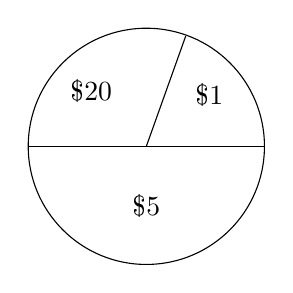
\begin{tikzpicture}
\draw (-1.5,0) -- (1.5,0);
\draw (0,0) -- (.5,1.4);
\draw (0,0) circle (1.5cm);
\draw (0,-.75) node {\$5};
\draw (-.7,.7) node {\$20};
\draw (.8,.65) node {\$1};
\end{tikzpicture}
\end{wrapfigure}

Sometimes taking a simple expected value makes sense.  Consider a
gamble in which one of three outcomes will occur. The outcomes are
worth \$1, \$5, and \$20 and the probabilities of the outcomes are .2,
.5, and .3, respectively. For example, a wheel is spun and the
probability of winning an amount corresponds to the area on the wheel.
The expected monetary value (EMV) of the gamble is
\[ \$1 \times .2 + \$5 \times .5 + \$20 \times .3 = \$8.70 \]

However, there exist situations where EMV is not an appropriate
indicator of ``fair value''. Consider another gamble in which a fair
coin is tossed until the first head appears. The gambler receives
$\$2^n$ where $n$ is the number of the tosses required until the first
instance of heads appears. So there will be $n-1$ tails followed by
heads. The probability of the first instance of heads occurring on
toss $n$ is $(1/2)^n$ and the EMV of the gamble is
\[
  2\left(\frac{1}{2}\right) + 4\left(\frac{1}{4}\right) + 8\left(\frac{1}{8}\right) +
  16\left(\frac{1}{16}\right) + \ldots = \infty.
\]
Few people (perhaps no one) would pay any amount to participate in the
gamble.  This is the St. Petersburg paradox stated by Bernoulli. To
resolve the paradox, he said that the monetary value is not as
important as the ``intrinsic worth'' of the money. For many people, an
increase in the amount of money has increasing worth, but at a
decreasing rate. Given an amount of money $m$, the logarithmic
function captures the basic relationship between $m$ and its
``intrinsic worth'' (see Figure~\vref{fig:diminishing}).

\begin{figure}
\centering
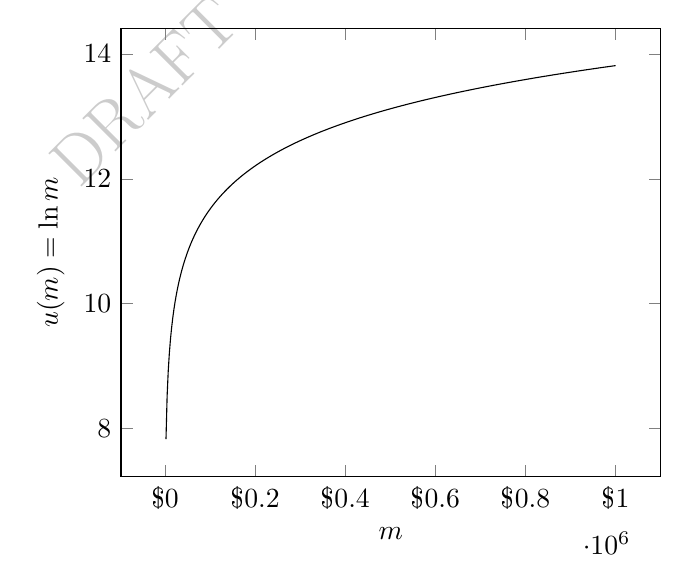
\begin{tikzpicture}
\begin{axis}[
    xlabel={$m$},
    ylabel={$u(m) = \ln m$},
    xticklabel={\$$\pgfmathprintnumber{\tick}$},
    %title={}
  ]
  \addplot[domain=0:1000000,samples=400] {ln(x)};
\end{axis}
\end{tikzpicture}
\caption{The diminishing rate of the value of money.}
\label{fig:diminishing}
\end{figure}

However, there are many functions with this basic shape and they
differ from person to person. How can the value (or utility) of money
be specified for an individual? Also, expected value is commonly
associated with value over the long run. What about a one-time
gamble? Von Neumann and Morgenstern (VnM~\cite{vonneumann:1953})
showed how to construst a utility that
represents a decision-maker's preferences (numerically) among gambles. Note that if
we were only concerned with choices among basic (certain) alternatives
then the decision-maker would simply rank the alternatives in an
ordinal manner. But we are concerned with decision-making under
risk. When we allow gambles, and ask a person to express preferences
over pairs of gambles (where the gambles are over basic alternatives)
then VnM showed how to associate utilities to the basic alternatives
in such a way that 
\begin{inparaenum}[1)] 
\item the utility for an alternative is measured by
the risk one is willing to take to receive it~\cite{savage:1972}, and
\item if decisions are made based on expected utility, then the
decision--maker is acting in agreement with her preferences.
\end{inparaenum}
Of course, the decision-maker's preferences must have some amount of
consistency. In other words, preferences must obey some rules that we
will state later.

Here is the basic idea for the construction of a utility function.
Suppose that among three different bands, Alice prefers
Smashing Pumpkins to Yo La Tengo, and she prefers Yo La Tengo to Wilco.
Now any three numbers that decrease in magnitude will capture
the ordinal preferences. But we are allowing gambles so that
we can capture Alice's attitude toward risk. We allow Alice
to choose between two alternatives 
\begin{inparaenum}[1)]
\item seeing Yo La Tengo for sure, or 
\item a gamble where she sees Smashing Pumpkins with probability
$p$ or Wilco with probability $1-p$. 
\end{inparaenum}
If $p$ is very close to one then Alice will choose the gamble. But if we
decrease $p$, then at \emph{some} point Alice will prefer the certain
alternative of seeing Yo La Tengo. We ask Alice for the value of
$p$ at which she is indifferent between the certain alternative and
the gamble. Suppose Alice indicates
$p=2/3$. Now, arbitrarily associate the value 1 with Smashing Pumpkins
and associate the value 0 with Wilco. Then it seems natural to
associate the value 2/3 with Yo La Tengo. Note that the value of Yo La
Tengo equals the expected value of the gamble.
\[ \frac{2}{3} = 1\left(\frac{2}{3}\right) +
  0\left(\frac{1}{3}\right) \] Instead of using (1, 2/3, 0) we could
use \emph{any} three numbers $a+c,~(2/3)a+c,~c$, where $a$ and
$c$ are constants and
$a>0$, and not alter the preferences (including the preference over the
certain outcome and the gamble).

Perhaps the most troublesome aspect of constructing utilities in this
way is the natural inclination to think about the utility values in
terms of ratios. You should avoid doing this.  For example, it is
\emph{not} correct to say that Alice prefers seeing Yo La Tengo to
seeing Wilco twice as much as she prefers seeing Smashing Pumpkins to
seeing Yo La Tengo. No! The number 2/3 reflects Alice's attitude
toward gambling, not her attitude toward the two intervals. A commonly
used example~\cite{luce:1957} to illustrate this fact is the
following. Suppose you like taking chances. You are
indifferent between 1) receiving \$9 for sure, or 2) participating in
a gamble that results in equal chances of receiving either \$10 or
nothing. Your utilities for the three amounts \$10, \$9 and \$0 are 1,
1/2, and 0, respectively. It's not that you have equal preferences
for going from \$0 to \$9 and going from \$9 to \$10. No. You simply
like taking chances.

Another common mistake is to say that Alice prefers Smashing Pumpkins
to Yo La Tengo because Smashing Pumpkins has higher utility. No!
Alice's preferences (and your preferences) among basic alternatives
and lotteries come first. A decision-maker knows her preferences. The
point is that if Alice can state her preferences, then we can
construct a numerical characterization of them. That is to say, we can
associate a value (i.e. a number) to something that is inherently
non-numeric.  The expected utility theorem is a representation
theorem.

\label{rules-of-consistency}
Now for the rules of consistency. Let $L(p,x,y)$ represent a gamble
(also called a lottery) in which you receive outcome $x$ with
probability $p$ or you receive outcome $y$ with probability
$(1-p)$. Also, let $x \succ y$ indicate that outcome $x$ is preferred
to outcome $y$, and let $x \sim y$ indicate indifference between the
outcomes $x$ and $y$. A decision-maker's preferences must satisfy the
following rules. (Note that the rules don't seem too objectionable).
\begin{enumerate}
\item $x \succ y$ or $y \succ x$ or $x \sim y$. (completeness)
\item if $x \succ y$ and $y \succ z$ then $x \succ z$. (transitivity)
\item $L\left(p,L(q,x,y),L(r,x,y)\right) \sim L(s,x,y)$ where $s=pq+(1-p)r$. (no fun in gambling)
\item given $x \succ y \succ z$, there is some lottery $L(p,x,z) \sim y$. (continuity)
\item if two lotteries are identical except for the first prize, then the
  lottery with the better first prize is preferred. (better prizes condition)
\item if two lotteries have the same alternatives as prizes, then the
  lottery that assigns higher probability of winning the best prize is
  preferred. (better chances condition)
\end{enumerate}
If you can state your preferences according to the above rules,
then an \emph{interval} utility function $u()$ can be constructed
in such a way that
\begin{enumerate}[i)]
\item $u(x) \succ u(y) \iff x \succ y$ \label{eu1}
\item $u(x) = u(y) \iff x \sim y$ \label{eu2}
\item $u\left(L(p,x,y)\right) = pu(x) + (1-p)u(y)$ 
(expected utility property) \label{eu3}
\item if $u'()$ is a positive linear transformation of $u()$ then
  $u'()$ also satisfies \ref{eu1}, \ref{eu2}, and \ref{eu3}. \label{eu4}
\end{enumerate}
Items \ref{eu1} through \ref{eu4} constitute the Expected Utility
Theorem.  When working through exercises, perhaps the most useful item is
item \ref{eu3}, the expected utility property. It states that the utility
of a lottery is equal to its expected utility. Do \emph{not} confuse
expected utility with the utility of the expected value, which is not
of interest.

\emph{Retirement and risk}.  This example is inspired from the
discussion on utility in Chernoff and Moses~\cite{chernoff:1959}.
Alice currently has \$\num{400000} in her individual retirement
account (IRA). Of course, it is always better to have more money for
retirement, but Alice is not super-greedy; she wants to have enough
money to pay bills and take a few backpacking trips each year.  Her
utility for an amount of money $m$ in the range \$0 to \$1 million is
given by the following function and is shown in
Figure~\vref{fig:retirement}.

\[
u(m) = \frac{10}{1+e^{-(\frac{m}{\num{500000}}-5)}}
\]

\begin{figure}
\centering
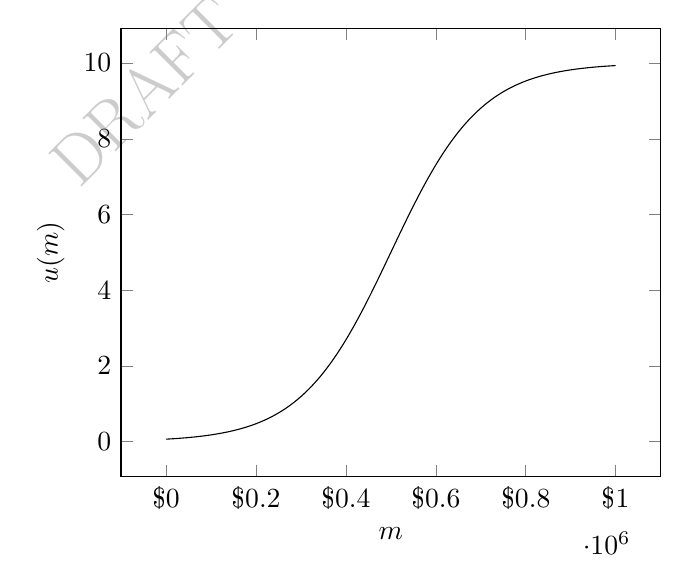
\begin{tikzpicture}
\begin{axis}[
    xlabel={$m$},
    ylabel={$u(m)$},
    xticklabel={\$$\pgfmathprintnumber{\tick}$},
    %title={Utility function for the retirement funds}
  ]
  %\addplot[domain=0:1000000,samples=1000] {10 / (1 + exp(-(x/500000 - 5)))};
  % tikz was plottting the function incorrectly, so for now i am resorting
  % to coordinates.
  \addplot[color=black,mark=none]
  coordinates {
(0,0.0669)(1000,0.0676)(2000,0.0683)(3000,0.069)(4000,0.0696)
(5000,0.0703)(6000,0.071)(7000,0.0717)(8000,0.0725)(9000,0.0732)
(10000,0.0739)(11000,0.0747)(12000,0.0754)(13000,0.0761)(14000,0.0769)
(15000,0.0777)(16000,0.0785)(17000,0.0792)(18000,0.08)(19000,0.0808)
(20000,0.0816)(21000,0.0824)(22000,0.0833)(23000,0.0841)(24000,0.0849)
(25000,0.0858)(26000,0.0866)(27000,0.0875)(28000,0.0884)(29000,0.0892)
(30000,0.0901)(31000,0.091)(32000,0.0919)(33000,0.0929)(34000,0.0938)
(35000,0.0947)(36000,0.0957)(37000,0.0966)(38000,0.0976)(39000,0.0985)
(40000,0.0995)(41000,0.1005)(42000,0.1015)(43000,0.1025)(44000,0.1035)
(45000,0.1046)(46000,0.1056)(47000,0.1067)(48000,0.1077)(49000,0.1088)
(50000,0.1099)(51000,0.111)(52000,0.1121)(53000,0.1132)(54000,0.1143)
(55000,0.1154)(56000,0.1166)(57000,0.1177)(58000,0.1189)(59000,0.1201)
(60000,0.1213)(61000,0.1225)(62000,0.1237)(63000,0.1249)(64000,0.1262)
(65000,0.1274)(66000,0.1287)(67000,0.13)(68000,0.1313)(69000,0.1326)
(70000,0.1339)(71000,0.1352)(72000,0.1365)(73000,0.1379)(74000,0.1393)
(75000,0.1406)(76000,0.142)(77000,0.1434)(78000,0.1449)(79000,0.1463)
(80000,0.1477)(81000,0.1492)(82000,0.1507)(83000,0.1522)(84000,0.1537)
(85000,0.1552)(86000,0.1567)(87000,0.1583)(88000,0.1598)(89000,0.1614)
(90000,0.163)(91000,0.1646)(92000,0.1663)(93000,0.1679)(94000,0.1696)
(95000,0.1712)(96000,0.1729)(97000,0.1746)(98000,0.1764)(99000,0.1781)
(1e+05,0.1799)(101000,0.1816)(102000,0.1834)(103000,0.1852)(104000,0.1871)
(105000,0.1889)(106000,0.1908)(107000,0.1927)(108000,0.1946)(109000,0.1965)
(110000,0.1984)(111000,0.2004)(112000,0.2023)(113000,0.2043)(114000,0.2063)
(115000,0.2084)(116000,0.2104)(117000,0.2125)(118000,0.2146)(119000,0.2167)
(120000,0.2188)(121000,0.221)(122000,0.2231)(123000,0.2253)(124000,0.2275)
(125000,0.2298)(126000,0.232)(127000,0.2343)(128000,0.2366)(129000,0.2389)
(130000,0.2413)(131000,0.2436)(132000,0.246)(133000,0.2484)(134000,0.2509)
(135000,0.2533)(136000,0.2558)(137000,0.2583)(138000,0.2608)(139000,0.2634)
(140000,0.266)(141000,0.2686)(142000,0.2712)(143000,0.2738)(144000,0.2765)
(145000,0.2792)(146000,0.282)(147000,0.2847)(148000,0.2875)(149000,0.2903)
(150000,0.2931)(151000,0.296)(152000,0.2989)(153000,0.3018)(154000,0.3047)
(155000,0.3077)(156000,0.3107)(157000,0.3137)(158000,0.3168)(159000,0.3198)
(160000,0.323)(161000,0.3261)(162000,0.3293)(163000,0.3325)(164000,0.3357)
(165000,0.339)(166000,0.3422)(167000,0.3456)(168000,0.3489)(169000,0.3523)
(170000,0.3557)(171000,0.3592)(172000,0.3626)(173000,0.3661)(174000,0.3697)
(175000,0.3733)(176000,0.3769)(177000,0.3805)(178000,0.3842)(179000,0.3879)
(180000,0.3917)(181000,0.3954)(182000,0.3993)(183000,0.4031)(184000,0.407)
(185000,0.4109)(186000,0.4149)(187000,0.4189)(188000,0.4229)(189000,0.427)
(190000,0.4311)(191000,0.4352)(192000,0.4394)(193000,0.4436)(194000,0.4479)
(195000,0.4522)(196000,0.4565)(197000,0.4609)(198000,0.4653)(199000,0.4698)
(2e+05,0.4743)(201000,0.4788)(202000,0.4834)(203000,0.488)(204000,0.4927)
(205000,0.4974)(206000,0.5021)(207000,0.5069)(208000,0.5117)(209000,0.5166)
(210000,0.5215)(211000,0.5265)(212000,0.5315)(213000,0.5366)(214000,0.5417)
(215000,0.5468)(216000,0.552)(217000,0.5572)(218000,0.5625)(219000,0.5679)
(220000,0.5732)(221000,0.5787)(222000,0.5841)(223000,0.5897)(224000,0.5952)
(225000,0.6009)(226000,0.6065)(227000,0.6123)(228000,0.618)(229000,0.6239)
(230000,0.6297)(231000,0.6357)(232000,0.6416)(233000,0.6477)(234000,0.6538)
(235000,0.6599)(236000,0.6661)(237000,0.6723)(238000,0.6786)(239000,0.685)
(240000,0.6914)(241000,0.6978)(242000,0.7044)(243000,0.7109)(244000,0.7176)
(245000,0.7243)(246000,0.731)(247000,0.7378)(248000,0.7447)(249000,0.7516)
(250000,0.7586)(251000,0.7656)(252000,0.7727)(253000,0.7799)(254000,0.7871)
(255000,0.7944)(256000,0.8017)(257000,0.8091)(258000,0.8166)(259000,0.8241)
(260000,0.8317)(261000,0.8394)(262000,0.8471)(263000,0.8549)(264000,0.8627)
(265000,0.8707)(266000,0.8786)(267000,0.8867)(268000,0.8948)(269000,0.903)
(270000,0.9112)(271000,0.9195)(272000,0.9279)(273000,0.9364)(274000,0.9449)
(275000,0.9535)(276000,0.9622)(277000,0.9709)(278000,0.9797)(279000,0.9886)
(280000,0.9975)(281000,1.0065)(282000,1.0156)(283000,1.0248)(284000,1.034)
(285000,1.0433)(286000,1.0527)(287000,1.0621)(288000,1.0717)(289000,1.0813)
(290000,1.091)(291000,1.1007)(292000,1.1106)(293000,1.1205)(294000,1.1305)
(295000,1.1405)(296000,1.1507)(297000,1.1609)(298000,1.1712)(299000,1.1816)
(3e+05,1.192)(301000,1.2026)(302000,1.2132)(303000,1.2239)(304000,1.2347)
(305000,1.2455)(306000,1.2565)(307000,1.2675)(308000,1.2786)(309000,1.2898)
(310000,1.3011)(311000,1.3124)(312000,1.3239)(313000,1.3354)(314000,1.347)
(315000,1.3587)(316000,1.3705)(317000,1.3824)(318000,1.3943)(319000,1.4064)
(320000,1.4185)(321000,1.4307)(322000,1.443)(323000,1.4554)(324000,1.4679)
(325000,1.4805)(326000,1.4931)(327000,1.5059)(328000,1.5187)(329000,1.5316)
(330000,1.5447)(331000,1.5578)(332000,1.571)(333000,1.5842)(334000,1.5976)
(335000,1.6111)(336000,1.6247)(337000,1.6383)(338000,1.652)(339000,1.6659)
(340000,1.6798)(341000,1.6938)(342000,1.708)(343000,1.7222)(344000,1.7365)
(345000,1.7509)(346000,1.7654)(347000,1.7799)(348000,1.7946)(349000,1.8094)
(350000,1.8243)(351000,1.8392)(352000,1.8543)(353000,1.8694)(354000,1.8847)
(355000,1.9)(356000,1.9155)(357000,1.931)(358000,1.9466)(359000,1.9623)
(360000,1.9782)(361000,1.9941)(362000,2.0101)(363000,2.0262)(364000,2.0424)
(365000,2.0587)(366000,2.0751)(367000,2.0916)(368000,2.1082)(369000,2.1249)
(370000,2.1417)(371000,2.1585)(372000,2.1755)(373000,2.1926)(374000,2.2097)
(375000,2.227)(376000,2.2444)(377000,2.2618)(378000,2.2794)(379000,2.297)
(380000,2.3148)(381000,2.3326)(382000,2.3505)(383000,2.3685)(384000,2.3867)
(385000,2.4049)(386000,2.4232)(387000,2.4416)(388000,2.4601)(389000,2.4787)
(390000,2.4974)(391000,2.5162)(392000,2.5351)(393000,2.554)(394000,2.5731)
(395000,2.5923)(396000,2.6115)(397000,2.6308)(398000,2.6503)(399000,2.6698)
(4e+05,2.6894)(401000,2.7091)(402000,2.7289)(403000,2.7488)(404000,2.7688)
(405000,2.7888)(406000,2.809)(407000,2.8292)(408000,2.8496)(409000,2.87)
(410000,2.8905)(411000,2.9111)(412000,2.9318)(413000,2.9525)(414000,2.9734)
(415000,2.9943)(416000,3.0153)(417000,3.0365)(418000,3.0576)(419000,3.0789)
(420000,3.1003)(421000,3.1217)(422000,3.1432)(423000,3.1648)(424000,3.1865)
(425000,3.2082)(426000,3.23)(427000,3.2519)(428000,3.2739)(429000,3.296)
(430000,3.3181)(431000,3.3403)(432000,3.3626)(433000,3.385)(434000,3.4074)
(435000,3.4299)(436000,3.4525)(437000,3.4751)(438000,3.4978)(439000,3.5206)
(440000,3.5434)(441000,3.5663)(442000,3.5893)(443000,3.6124)(444000,3.6355)
(445000,3.6586)(446000,3.6819)(447000,3.7052)(448000,3.7285)(449000,3.7519)
(450000,3.7754)(451000,3.7989)(452000,3.8225)(453000,3.8462)(454000,3.8699)
(455000,3.8936)(456000,3.9174)(457000,3.9413)(458000,3.9652)(459000,3.9891)
(460000,4.0131)(461000,4.0372)(462000,4.0613)(463000,4.0854)(464000,4.1096)
(465000,4.1338)(466000,4.1581)(467000,4.1824)(468000,4.2068)(469000,4.2311)
(470000,4.2556)(471000,4.28)(472000,4.3045)(473000,4.3291)(474000,4.3536)
(475000,4.3782)(476000,4.4029)(477000,4.4275)(478000,4.4522)(479000,4.4769)
(480000,4.5017)(481000,4.5264)(482000,4.5512)(483000,4.576)(484000,4.6009)
(485000,4.6257)(486000,4.6506)(487000,4.6755)(488000,4.7004)(489000,4.7253)
(490000,4.7502)(491000,4.7752)(492000,4.8001)(493000,4.8251)(494000,4.85)
(495000,4.875)(496000,4.9)(497000,4.925)(498000,4.95)(499000,4.975)
(5e+05,5)(501000,5.025)(502000,5.05)(503000,5.075)(504000,5.1)
(505000,5.125)(506000,5.15)(507000,5.1749)(508000,5.1999)(509000,5.2248)
(510000,5.2498)(511000,5.2747)(512000,5.2996)(513000,5.3245)(514000,5.3494)
(515000,5.3743)(516000,5.3991)(517000,5.424)(518000,5.4488)(519000,5.4736)
(520000,5.4983)(521000,5.5231)(522000,5.5478)(523000,5.5725)(524000,5.5971)
(525000,5.6218)(526000,5.6464)(527000,5.6709)(528000,5.6955)(529000,5.72)
(530000,5.7444)(531000,5.7689)(532000,5.7932)(533000,5.8176)(534000,5.8419)
(535000,5.8662)(536000,5.8904)(537000,5.9146)(538000,5.9387)(539000,5.9628)
(540000,5.9869)(541000,6.0109)(542000,6.0348)(543000,6.0587)(544000,6.0826)
(545000,6.1064)(546000,6.1301)(547000,6.1538)(548000,6.1775)(549000,6.2011)
(550000,6.2246)(551000,6.2481)(552000,6.2715)(553000,6.2948)(554000,6.3181)
(555000,6.3414)(556000,6.3645)(557000,6.3876)(558000,6.4107)(559000,6.4337)
(560000,6.4566)(561000,6.4794)(562000,6.5022)(563000,6.5249)(564000,6.5475)
(565000,6.5701)(566000,6.5926)(567000,6.615)(568000,6.6374)(569000,6.6597)
(570000,6.6819)(571000,6.704)(572000,6.7261)(573000,6.7481)(574000,6.77)
(575000,6.7918)(576000,6.8135)(577000,6.8352)(578000,6.8568)(579000,6.8783)
(580000,6.8997)(581000,6.9211)(582000,6.9424)(583000,6.9635)(584000,6.9847)
(585000,7.0057)(586000,7.0266)(587000,7.0475)(588000,7.0682)(589000,7.0889)
(590000,7.1095)(591000,7.13)(592000,7.1504)(593000,7.1708)(594000,7.191)
(595000,7.2112)(596000,7.2312)(597000,7.2512)(598000,7.2711)(599000,7.2909)
(6e+05,7.3106)(601000,7.3302)(602000,7.3497)(603000,7.3692)(604000,7.3885)
(605000,7.4077)(606000,7.4269)(607000,7.446)(608000,7.4649)(609000,7.4838)
(610000,7.5026)(611000,7.5213)(612000,7.5399)(613000,7.5584)(614000,7.5768)
(615000,7.5951)(616000,7.6133)(617000,7.6315)(618000,7.6495)(619000,7.6674)
(620000,7.6852)(621000,7.703)(622000,7.7206)(623000,7.7382)(624000,7.7556)
(625000,7.773)(626000,7.7903)(627000,7.8074)(628000,7.8245)(629000,7.8415)
(630000,7.8583)(631000,7.8751)(632000,7.8918)(633000,7.9084)(634000,7.9249)
(635000,7.9413)(636000,7.9576)(637000,7.9738)(638000,7.9899)(639000,8.0059)
(640000,8.0218)(641000,8.0377)(642000,8.0534)(643000,8.069)(644000,8.0845)
(645000,8.1)(646000,8.1153)(647000,8.1306)(648000,8.1457)(649000,8.1608)
(650000,8.1757)(651000,8.1906)(652000,8.2054)(653000,8.2201)(654000,8.2346)
(655000,8.2491)(656000,8.2635)(657000,8.2778)(658000,8.292)(659000,8.3062)
(660000,8.3202)(661000,8.3341)(662000,8.348)(663000,8.3617)(664000,8.3753)
(665000,8.3889)(666000,8.4024)(667000,8.4158)(668000,8.429)(669000,8.4422)
(670000,8.4553)(671000,8.4684)(672000,8.4813)(673000,8.4941)(674000,8.5069)
(675000,8.5195)(676000,8.5321)(677000,8.5446)(678000,8.557)(679000,8.5693)
(680000,8.5815)(681000,8.5936)(682000,8.6057)(683000,8.6176)(684000,8.6295)
(685000,8.6413)(686000,8.653)(687000,8.6646)(688000,8.6761)(689000,8.6876)
(690000,8.6989)(691000,8.7102)(692000,8.7214)(693000,8.7325)(694000,8.7435)
(695000,8.7545)(696000,8.7653)(697000,8.7761)(698000,8.7868)(699000,8.7974)
(7e+05,8.808)(701000,8.8184)(702000,8.8288)(703000,8.8391)(704000,8.8493)
(705000,8.8595)(706000,8.8695)(707000,8.8795)(708000,8.8894)(709000,8.8993)
(710000,8.909)(711000,8.9187)(712000,8.9283)(713000,8.9379)(714000,8.9473)
(715000,8.9567)(716000,8.966)(717000,8.9752)(718000,8.9844)(719000,8.9935)
(720000,9.0025)(721000,9.0114)(722000,9.0203)(723000,9.0291)(724000,9.0378)
(725000,9.0465)(726000,9.0551)(727000,9.0636)(728000,9.0721)(729000,9.0805)
(730000,9.0888)(731000,9.097)(732000,9.1052)(733000,9.1133)(734000,9.1214)
(735000,9.1293)(736000,9.1373)(737000,9.1451)(738000,9.1529)(739000,9.1606)
(740000,9.1683)(741000,9.1759)(742000,9.1834)(743000,9.1909)(744000,9.1983)
(745000,9.2056)(746000,9.2129)(747000,9.2201)(748000,9.2273)(749000,9.2344)
(750000,9.2414)(751000,9.2484)(752000,9.2553)(753000,9.2622)(754000,9.269)
(755000,9.2757)(756000,9.2824)(757000,9.2891)(758000,9.2956)(759000,9.3022)
(760000,9.3086)(761000,9.315)(762000,9.3214)(763000,9.3277)(764000,9.3339)
(765000,9.3401)(766000,9.3462)(767000,9.3523)(768000,9.3584)(769000,9.3643)
(770000,9.3703)(771000,9.3761)(772000,9.382)(773000,9.3877)(774000,9.3935)
(775000,9.3991)(776000,9.4048)(777000,9.4103)(778000,9.4159)(779000,9.4213)
(780000,9.4268)(781000,9.4321)(782000,9.4375)(783000,9.4428)(784000,9.448)
(785000,9.4532)(786000,9.4583)(787000,9.4634)(788000,9.4685)(789000,9.4735)
(790000,9.4785)(791000,9.4834)(792000,9.4883)(793000,9.4931)(794000,9.4979)
(795000,9.5026)(796000,9.5073)(797000,9.512)(798000,9.5166)(799000,9.5212)
(8e+05,9.5257)(801000,9.5302)(802000,9.5347)(803000,9.5391)(804000,9.5435)
(805000,9.5478)(806000,9.5521)(807000,9.5564)(808000,9.5606)(809000,9.5648)
(810000,9.5689)(811000,9.573)(812000,9.5771)(813000,9.5811)(814000,9.5851)
(815000,9.5891)(816000,9.593)(817000,9.5969)(818000,9.6007)(819000,9.6046)
(820000,9.6083)(821000,9.6121)(822000,9.6158)(823000,9.6195)(824000,9.6231)
(825000,9.6267)(826000,9.6303)(827000,9.6339)(828000,9.6374)(829000,9.6408)
(830000,9.6443)(831000,9.6477)(832000,9.6511)(833000,9.6544)(834000,9.6578)
(835000,9.661)(836000,9.6643)(837000,9.6675)(838000,9.6707)(839000,9.6739)
(840000,9.677)(841000,9.6802)(842000,9.6832)(843000,9.6863)(844000,9.6893)
(845000,9.6923)(846000,9.6953)(847000,9.6982)(848000,9.7011)(849000,9.704)
(850000,9.7069)(851000,9.7097)(852000,9.7125)(853000,9.7153)(854000,9.718)
(855000,9.7208)(856000,9.7235)(857000,9.7262)(858000,9.7288)(859000,9.7314)
(860000,9.734)(861000,9.7366)(862000,9.7392)(863000,9.7417)(864000,9.7442)
(865000,9.7467)(866000,9.7491)(867000,9.7516)(868000,9.754)(869000,9.7564)
(870000,9.7587)(871000,9.7611)(872000,9.7634)(873000,9.7657)(874000,9.768)
(875000,9.7702)(876000,9.7725)(877000,9.7747)(878000,9.7769)(879000,9.779)
(880000,9.7812)(881000,9.7833)(882000,9.7854)(883000,9.7875)(884000,9.7896)
(885000,9.7916)(886000,9.7937)(887000,9.7957)(888000,9.7977)(889000,9.7996)
(890000,9.8016)(891000,9.8035)(892000,9.8054)(893000,9.8073)(894000,9.8092)
(895000,9.8111)(896000,9.8129)(897000,9.8148)(898000,9.8166)(899000,9.8184)
(9e+05,9.8201)(901000,9.8219)(902000,9.8236)(903000,9.8254)(904000,9.8271)
(905000,9.8288)(906000,9.8304)(907000,9.8321)(908000,9.8337)(909000,9.8354)
(910000,9.837)(911000,9.8386)(912000,9.8402)(913000,9.8417)(914000,9.8433)
(915000,9.8448)(916000,9.8463)(917000,9.8478)(918000,9.8493)(919000,9.8508)
(920000,9.8523)(921000,9.8537)(922000,9.8551)(923000,9.8566)(924000,9.858)
(925000,9.8594)(926000,9.8607)(927000,9.8621)(928000,9.8635)(929000,9.8648)
(930000,9.8661)(931000,9.8674)(932000,9.8687)(933000,9.87)(934000,9.8713)
(935000,9.8726)(936000,9.8738)(937000,9.8751)(938000,9.8763)(939000,9.8775)
(940000,9.8787)(941000,9.8799)(942000,9.8811)(943000,9.8823)(944000,9.8834)
(945000,9.8846)(946000,9.8857)(947000,9.8868)(948000,9.8879)(949000,9.889)
(950000,9.8901)(951000,9.8912)(952000,9.8923)(953000,9.8933)(954000,9.8944)
(955000,9.8954)(956000,9.8965)(957000,9.8975)(958000,9.8985)(959000,9.8995)
(960000,9.9005)(961000,9.9015)(962000,9.9024)(963000,9.9034)(964000,9.9043)
(965000,9.9053)(966000,9.9062)(967000,9.9071)(968000,9.9081)(969000,9.909)
(970000,9.9099)(971000,9.9108)(972000,9.9116)(973000,9.9125)(974000,9.9134)
(975000,9.9142)(976000,9.9151)(977000,9.9159)(978000,9.9167)(979000,9.9176)
(980000,9.9184)(981000,9.9192)(982000,9.92)(983000,9.9208)(984000,9.9215)
(985000,9.9223)(986000,9.9231)(987000,9.9239)(988000,9.9246)(989000,9.9253)
(990000,9.9261)(991000,9.9268)(992000,9.9275)(993000,9.9283)(994000,9.929)
(995000,9.9297)(996000,9.9304)(997000,9.931)(998000,9.9317)(999000,9.9324)
(1e+06,9.9331)
  };
\end{axis}
\end{tikzpicture}
\caption{Utility function for the retirement funds.}
\label{fig:retirement}
\end{figure}

Note that her current utility is
$u(\$\num{400000})=2.69$.  Suppose that on a trip to Las Vegas, Alice
is offered a gambling opportunity for gaining \$\num{200000} or losing
\$\num{100000}. The odds are 1-to-1 for gaining and losing. If Alice wins,
she will have \$\num{600000}, but if she loses, she will have
\$\num{300000}. Alice knows about the the expected utility property:
that the utility of a lottery is equal to its expected
utility. Converting from odds to probabilities, she computes the
utility of the gamble as
\[
\frac{1}{2}u(\$\num{600000}) + \frac{1}{2}u(\$\num{300000}) = 4.25,
\]
which is higher than her current utility so she takes the gamble.

Suppose that Alice wins. She now had \$\num{600000} and her utility is
$u(\$\num{600000}) = 7.31$.  
Gaining confidence in her luck, Alice seeks and finds another
opportunity. The new gamble has odds of 1-to-2 for winning
\$\num{200000} or losing \$\num{100000}. 
The probability $p$ of winning is
\[
p = \frac{\text{odds}}{\text{odds}+1} = 
\frac{\frac{1}{2}}{\frac{1}{2} + 1} = \frac{1}{3}.
\]
Notice that the gamble is fair because
\[
\frac{1}{3}u(\$\num{200000}) - \frac{2}{3}u(\$\num{100000}) = 0.
\]
\emph{Alice's} utility for the new opportunity is
\[
\frac{1}{3}u(\$\num{800000}) + \frac{2}{3}u(\$\num{500000}) = 6.51,
\]
which is less than her current utility and so, even though
the gamble is fair, she declines.

\tikzstyle{place}=[circle,draw,minimum size=.75mm,
  inner sep=0pt,fill=black]
\begin{figure}
\centering
\begin{tikzpicture}
\begin{axis}[
    xlabel={$m$},
    ylabel={$u(m)$},
    xticklabel={\$$\pgfmathprintnumber{\tick}$},
    %title={A graphic interpretation of the gamble}
  ]
  \addplot[color=black,mark=none]
  coordinates {
(0,0.0669)(1000,0.0676)(2000,0.0683)(3000,0.069)(4000,0.0696)
(5000,0.0703)(6000,0.071)(7000,0.0717)(8000,0.0725)(9000,0.0732)
(10000,0.0739)(11000,0.0747)(12000,0.0754)(13000,0.0761)(14000,0.0769)
(15000,0.0777)(16000,0.0785)(17000,0.0792)(18000,0.08)(19000,0.0808)
(20000,0.0816)(21000,0.0824)(22000,0.0833)(23000,0.0841)(24000,0.0849)
(25000,0.0858)(26000,0.0866)(27000,0.0875)(28000,0.0884)(29000,0.0892)
(30000,0.0901)(31000,0.091)(32000,0.0919)(33000,0.0929)(34000,0.0938)
(35000,0.0947)(36000,0.0957)(37000,0.0966)(38000,0.0976)(39000,0.0985)
(40000,0.0995)(41000,0.1005)(42000,0.1015)(43000,0.1025)(44000,0.1035)
(45000,0.1046)(46000,0.1056)(47000,0.1067)(48000,0.1077)(49000,0.1088)
(50000,0.1099)(51000,0.111)(52000,0.1121)(53000,0.1132)(54000,0.1143)
(55000,0.1154)(56000,0.1166)(57000,0.1177)(58000,0.1189)(59000,0.1201)
(60000,0.1213)(61000,0.1225)(62000,0.1237)(63000,0.1249)(64000,0.1262)
(65000,0.1274)(66000,0.1287)(67000,0.13)(68000,0.1313)(69000,0.1326)
(70000,0.1339)(71000,0.1352)(72000,0.1365)(73000,0.1379)(74000,0.1393)
(75000,0.1406)(76000,0.142)(77000,0.1434)(78000,0.1449)(79000,0.1463)
(80000,0.1477)(81000,0.1492)(82000,0.1507)(83000,0.1522)(84000,0.1537)
(85000,0.1552)(86000,0.1567)(87000,0.1583)(88000,0.1598)(89000,0.1614)
(90000,0.163)(91000,0.1646)(92000,0.1663)(93000,0.1679)(94000,0.1696)
(95000,0.1712)(96000,0.1729)(97000,0.1746)(98000,0.1764)(99000,0.1781)
(1e+05,0.1799)(101000,0.1816)(102000,0.1834)(103000,0.1852)(104000,0.1871)
(105000,0.1889)(106000,0.1908)(107000,0.1927)(108000,0.1946)(109000,0.1965)
(110000,0.1984)(111000,0.2004)(112000,0.2023)(113000,0.2043)(114000,0.2063)
(115000,0.2084)(116000,0.2104)(117000,0.2125)(118000,0.2146)(119000,0.2167)
(120000,0.2188)(121000,0.221)(122000,0.2231)(123000,0.2253)(124000,0.2275)
(125000,0.2298)(126000,0.232)(127000,0.2343)(128000,0.2366)(129000,0.2389)
(130000,0.2413)(131000,0.2436)(132000,0.246)(133000,0.2484)(134000,0.2509)
(135000,0.2533)(136000,0.2558)(137000,0.2583)(138000,0.2608)(139000,0.2634)
(140000,0.266)(141000,0.2686)(142000,0.2712)(143000,0.2738)(144000,0.2765)
(145000,0.2792)(146000,0.282)(147000,0.2847)(148000,0.2875)(149000,0.2903)
(150000,0.2931)(151000,0.296)(152000,0.2989)(153000,0.3018)(154000,0.3047)
(155000,0.3077)(156000,0.3107)(157000,0.3137)(158000,0.3168)(159000,0.3198)
(160000,0.323)(161000,0.3261)(162000,0.3293)(163000,0.3325)(164000,0.3357)
(165000,0.339)(166000,0.3422)(167000,0.3456)(168000,0.3489)(169000,0.3523)
(170000,0.3557)(171000,0.3592)(172000,0.3626)(173000,0.3661)(174000,0.3697)
(175000,0.3733)(176000,0.3769)(177000,0.3805)(178000,0.3842)(179000,0.3879)
(180000,0.3917)(181000,0.3954)(182000,0.3993)(183000,0.4031)(184000,0.407)
(185000,0.4109)(186000,0.4149)(187000,0.4189)(188000,0.4229)(189000,0.427)
(190000,0.4311)(191000,0.4352)(192000,0.4394)(193000,0.4436)(194000,0.4479)
(195000,0.4522)(196000,0.4565)(197000,0.4609)(198000,0.4653)(199000,0.4698)
(2e+05,0.4743)(201000,0.4788)(202000,0.4834)(203000,0.488)(204000,0.4927)
(205000,0.4974)(206000,0.5021)(207000,0.5069)(208000,0.5117)(209000,0.5166)
(210000,0.5215)(211000,0.5265)(212000,0.5315)(213000,0.5366)(214000,0.5417)
(215000,0.5468)(216000,0.552)(217000,0.5572)(218000,0.5625)(219000,0.5679)
(220000,0.5732)(221000,0.5787)(222000,0.5841)(223000,0.5897)(224000,0.5952)
(225000,0.6009)(226000,0.6065)(227000,0.6123)(228000,0.618)(229000,0.6239)
(230000,0.6297)(231000,0.6357)(232000,0.6416)(233000,0.6477)(234000,0.6538)
(235000,0.6599)(236000,0.6661)(237000,0.6723)(238000,0.6786)(239000,0.685)
(240000,0.6914)(241000,0.6978)(242000,0.7044)(243000,0.7109)(244000,0.7176)
(245000,0.7243)(246000,0.731)(247000,0.7378)(248000,0.7447)(249000,0.7516)
(250000,0.7586)(251000,0.7656)(252000,0.7727)(253000,0.7799)(254000,0.7871)
(255000,0.7944)(256000,0.8017)(257000,0.8091)(258000,0.8166)(259000,0.8241)
(260000,0.8317)(261000,0.8394)(262000,0.8471)(263000,0.8549)(264000,0.8627)
(265000,0.8707)(266000,0.8786)(267000,0.8867)(268000,0.8948)(269000,0.903)
(270000,0.9112)(271000,0.9195)(272000,0.9279)(273000,0.9364)(274000,0.9449)
(275000,0.9535)(276000,0.9622)(277000,0.9709)(278000,0.9797)(279000,0.9886)
(280000,0.9975)(281000,1.0065)(282000,1.0156)(283000,1.0248)(284000,1.034)
(285000,1.0433)(286000,1.0527)(287000,1.0621)(288000,1.0717)(289000,1.0813)
(290000,1.091)(291000,1.1007)(292000,1.1106)(293000,1.1205)(294000,1.1305)
(295000,1.1405)(296000,1.1507)(297000,1.1609)(298000,1.1712)(299000,1.1816)
(3e+05,1.192)(301000,1.2026)(302000,1.2132)(303000,1.2239)(304000,1.2347)
(305000,1.2455)(306000,1.2565)(307000,1.2675)(308000,1.2786)(309000,1.2898)
(310000,1.3011)(311000,1.3124)(312000,1.3239)(313000,1.3354)(314000,1.347)
(315000,1.3587)(316000,1.3705)(317000,1.3824)(318000,1.3943)(319000,1.4064)
(320000,1.4185)(321000,1.4307)(322000,1.443)(323000,1.4554)(324000,1.4679)
(325000,1.4805)(326000,1.4931)(327000,1.5059)(328000,1.5187)(329000,1.5316)
(330000,1.5447)(331000,1.5578)(332000,1.571)(333000,1.5842)(334000,1.5976)
(335000,1.6111)(336000,1.6247)(337000,1.6383)(338000,1.652)(339000,1.6659)
(340000,1.6798)(341000,1.6938)(342000,1.708)(343000,1.7222)(344000,1.7365)
(345000,1.7509)(346000,1.7654)(347000,1.7799)(348000,1.7946)(349000,1.8094)
(350000,1.8243)(351000,1.8392)(352000,1.8543)(353000,1.8694)(354000,1.8847)
(355000,1.9)(356000,1.9155)(357000,1.931)(358000,1.9466)(359000,1.9623)
(360000,1.9782)(361000,1.9941)(362000,2.0101)(363000,2.0262)(364000,2.0424)
(365000,2.0587)(366000,2.0751)(367000,2.0916)(368000,2.1082)(369000,2.1249)
(370000,2.1417)(371000,2.1585)(372000,2.1755)(373000,2.1926)(374000,2.2097)
(375000,2.227)(376000,2.2444)(377000,2.2618)(378000,2.2794)(379000,2.297)
(380000,2.3148)(381000,2.3326)(382000,2.3505)(383000,2.3685)(384000,2.3867)
(385000,2.4049)(386000,2.4232)(387000,2.4416)(388000,2.4601)(389000,2.4787)
(390000,2.4974)(391000,2.5162)(392000,2.5351)(393000,2.554)(394000,2.5731)
(395000,2.5923)(396000,2.6115)(397000,2.6308)(398000,2.6503)(399000,2.6698)
(4e+05,2.6894)(401000,2.7091)(402000,2.7289)(403000,2.7488)(404000,2.7688)
(405000,2.7888)(406000,2.809)(407000,2.8292)(408000,2.8496)(409000,2.87)
(410000,2.8905)(411000,2.9111)(412000,2.9318)(413000,2.9525)(414000,2.9734)
(415000,2.9943)(416000,3.0153)(417000,3.0365)(418000,3.0576)(419000,3.0789)
(420000,3.1003)(421000,3.1217)(422000,3.1432)(423000,3.1648)(424000,3.1865)
(425000,3.2082)(426000,3.23)(427000,3.2519)(428000,3.2739)(429000,3.296)
(430000,3.3181)(431000,3.3403)(432000,3.3626)(433000,3.385)(434000,3.4074)
(435000,3.4299)(436000,3.4525)(437000,3.4751)(438000,3.4978)(439000,3.5206)
(440000,3.5434)(441000,3.5663)(442000,3.5893)(443000,3.6124)(444000,3.6355)
(445000,3.6586)(446000,3.6819)(447000,3.7052)(448000,3.7285)(449000,3.7519)
(450000,3.7754)(451000,3.7989)(452000,3.8225)(453000,3.8462)(454000,3.8699)
(455000,3.8936)(456000,3.9174)(457000,3.9413)(458000,3.9652)(459000,3.9891)
(460000,4.0131)(461000,4.0372)(462000,4.0613)(463000,4.0854)(464000,4.1096)
(465000,4.1338)(466000,4.1581)(467000,4.1824)(468000,4.2068)(469000,4.2311)
(470000,4.2556)(471000,4.28)(472000,4.3045)(473000,4.3291)(474000,4.3536)
(475000,4.3782)(476000,4.4029)(477000,4.4275)(478000,4.4522)(479000,4.4769)
(480000,4.5017)(481000,4.5264)(482000,4.5512)(483000,4.576)(484000,4.6009)
(485000,4.6257)(486000,4.6506)(487000,4.6755)(488000,4.7004)(489000,4.7253)
(490000,4.7502)(491000,4.7752)(492000,4.8001)(493000,4.8251)(494000,4.85)
(495000,4.875)(496000,4.9)(497000,4.925)(498000,4.95)(499000,4.975)
(5e+05,5)(501000,5.025)(502000,5.05)(503000,5.075)(504000,5.1)
(505000,5.125)(506000,5.15)(507000,5.1749)(508000,5.1999)(509000,5.2248)
(510000,5.2498)(511000,5.2747)(512000,5.2996)(513000,5.3245)(514000,5.3494)
(515000,5.3743)(516000,5.3991)(517000,5.424)(518000,5.4488)(519000,5.4736)
(520000,5.4983)(521000,5.5231)(522000,5.5478)(523000,5.5725)(524000,5.5971)
(525000,5.6218)(526000,5.6464)(527000,5.6709)(528000,5.6955)(529000,5.72)
(530000,5.7444)(531000,5.7689)(532000,5.7932)(533000,5.8176)(534000,5.8419)
(535000,5.8662)(536000,5.8904)(537000,5.9146)(538000,5.9387)(539000,5.9628)
(540000,5.9869)(541000,6.0109)(542000,6.0348)(543000,6.0587)(544000,6.0826)
(545000,6.1064)(546000,6.1301)(547000,6.1538)(548000,6.1775)(549000,6.2011)
(550000,6.2246)(551000,6.2481)(552000,6.2715)(553000,6.2948)(554000,6.3181)
(555000,6.3414)(556000,6.3645)(557000,6.3876)(558000,6.4107)(559000,6.4337)
(560000,6.4566)(561000,6.4794)(562000,6.5022)(563000,6.5249)(564000,6.5475)
(565000,6.5701)(566000,6.5926)(567000,6.615)(568000,6.6374)(569000,6.6597)
(570000,6.6819)(571000,6.704)(572000,6.7261)(573000,6.7481)(574000,6.77)
(575000,6.7918)(576000,6.8135)(577000,6.8352)(578000,6.8568)(579000,6.8783)
(580000,6.8997)(581000,6.9211)(582000,6.9424)(583000,6.9635)(584000,6.9847)
(585000,7.0057)(586000,7.0266)(587000,7.0475)(588000,7.0682)(589000,7.0889)
(590000,7.1095)(591000,7.13)(592000,7.1504)(593000,7.1708)(594000,7.191)
(595000,7.2112)(596000,7.2312)(597000,7.2512)(598000,7.2711)(599000,7.2909)
(6e+05,7.3106)(601000,7.3302)(602000,7.3497)(603000,7.3692)(604000,7.3885)
(605000,7.4077)(606000,7.4269)(607000,7.446)(608000,7.4649)(609000,7.4838)
(610000,7.5026)(611000,7.5213)(612000,7.5399)(613000,7.5584)(614000,7.5768)
(615000,7.5951)(616000,7.6133)(617000,7.6315)(618000,7.6495)(619000,7.6674)
(620000,7.6852)(621000,7.703)(622000,7.7206)(623000,7.7382)(624000,7.7556)
(625000,7.773)(626000,7.7903)(627000,7.8074)(628000,7.8245)(629000,7.8415)
(630000,7.8583)(631000,7.8751)(632000,7.8918)(633000,7.9084)(634000,7.9249)
(635000,7.9413)(636000,7.9576)(637000,7.9738)(638000,7.9899)(639000,8.0059)
(640000,8.0218)(641000,8.0377)(642000,8.0534)(643000,8.069)(644000,8.0845)
(645000,8.1)(646000,8.1153)(647000,8.1306)(648000,8.1457)(649000,8.1608)
(650000,8.1757)(651000,8.1906)(652000,8.2054)(653000,8.2201)(654000,8.2346)
(655000,8.2491)(656000,8.2635)(657000,8.2778)(658000,8.292)(659000,8.3062)
(660000,8.3202)(661000,8.3341)(662000,8.348)(663000,8.3617)(664000,8.3753)
(665000,8.3889)(666000,8.4024)(667000,8.4158)(668000,8.429)(669000,8.4422)
(670000,8.4553)(671000,8.4684)(672000,8.4813)(673000,8.4941)(674000,8.5069)
(675000,8.5195)(676000,8.5321)(677000,8.5446)(678000,8.557)(679000,8.5693)
(680000,8.5815)(681000,8.5936)(682000,8.6057)(683000,8.6176)(684000,8.6295)
(685000,8.6413)(686000,8.653)(687000,8.6646)(688000,8.6761)(689000,8.6876)
(690000,8.6989)(691000,8.7102)(692000,8.7214)(693000,8.7325)(694000,8.7435)
(695000,8.7545)(696000,8.7653)(697000,8.7761)(698000,8.7868)(699000,8.7974)
(7e+05,8.808)(701000,8.8184)(702000,8.8288)(703000,8.8391)(704000,8.8493)
(705000,8.8595)(706000,8.8695)(707000,8.8795)(708000,8.8894)(709000,8.8993)
(710000,8.909)(711000,8.9187)(712000,8.9283)(713000,8.9379)(714000,8.9473)
(715000,8.9567)(716000,8.966)(717000,8.9752)(718000,8.9844)(719000,8.9935)
(720000,9.0025)(721000,9.0114)(722000,9.0203)(723000,9.0291)(724000,9.0378)
(725000,9.0465)(726000,9.0551)(727000,9.0636)(728000,9.0721)(729000,9.0805)
(730000,9.0888)(731000,9.097)(732000,9.1052)(733000,9.1133)(734000,9.1214)
(735000,9.1293)(736000,9.1373)(737000,9.1451)(738000,9.1529)(739000,9.1606)
(740000,9.1683)(741000,9.1759)(742000,9.1834)(743000,9.1909)(744000,9.1983)
(745000,9.2056)(746000,9.2129)(747000,9.2201)(748000,9.2273)(749000,9.2344)
(750000,9.2414)(751000,9.2484)(752000,9.2553)(753000,9.2622)(754000,9.269)
(755000,9.2757)(756000,9.2824)(757000,9.2891)(758000,9.2956)(759000,9.3022)
(760000,9.3086)(761000,9.315)(762000,9.3214)(763000,9.3277)(764000,9.3339)
(765000,9.3401)(766000,9.3462)(767000,9.3523)(768000,9.3584)(769000,9.3643)
(770000,9.3703)(771000,9.3761)(772000,9.382)(773000,9.3877)(774000,9.3935)
(775000,9.3991)(776000,9.4048)(777000,9.4103)(778000,9.4159)(779000,9.4213)
(780000,9.4268)(781000,9.4321)(782000,9.4375)(783000,9.4428)(784000,9.448)
(785000,9.4532)(786000,9.4583)(787000,9.4634)(788000,9.4685)(789000,9.4735)
(790000,9.4785)(791000,9.4834)(792000,9.4883)(793000,9.4931)(794000,9.4979)
(795000,9.5026)(796000,9.5073)(797000,9.512)(798000,9.5166)(799000,9.5212)
(8e+05,9.5257)(801000,9.5302)(802000,9.5347)(803000,9.5391)(804000,9.5435)
(805000,9.5478)(806000,9.5521)(807000,9.5564)(808000,9.5606)(809000,9.5648)
(810000,9.5689)(811000,9.573)(812000,9.5771)(813000,9.5811)(814000,9.5851)
(815000,9.5891)(816000,9.593)(817000,9.5969)(818000,9.6007)(819000,9.6046)
(820000,9.6083)(821000,9.6121)(822000,9.6158)(823000,9.6195)(824000,9.6231)
(825000,9.6267)(826000,9.6303)(827000,9.6339)(828000,9.6374)(829000,9.6408)
(830000,9.6443)(831000,9.6477)(832000,9.6511)(833000,9.6544)(834000,9.6578)
(835000,9.661)(836000,9.6643)(837000,9.6675)(838000,9.6707)(839000,9.6739)
(840000,9.677)(841000,9.6802)(842000,9.6832)(843000,9.6863)(844000,9.6893)
(845000,9.6923)(846000,9.6953)(847000,9.6982)(848000,9.7011)(849000,9.704)
(850000,9.7069)(851000,9.7097)(852000,9.7125)(853000,9.7153)(854000,9.718)
(855000,9.7208)(856000,9.7235)(857000,9.7262)(858000,9.7288)(859000,9.7314)
(860000,9.734)(861000,9.7366)(862000,9.7392)(863000,9.7417)(864000,9.7442)
(865000,9.7467)(866000,9.7491)(867000,9.7516)(868000,9.754)(869000,9.7564)
(870000,9.7587)(871000,9.7611)(872000,9.7634)(873000,9.7657)(874000,9.768)
(875000,9.7702)(876000,9.7725)(877000,9.7747)(878000,9.7769)(879000,9.779)
(880000,9.7812)(881000,9.7833)(882000,9.7854)(883000,9.7875)(884000,9.7896)
(885000,9.7916)(886000,9.7937)(887000,9.7957)(888000,9.7977)(889000,9.7996)
(890000,9.8016)(891000,9.8035)(892000,9.8054)(893000,9.8073)(894000,9.8092)
(895000,9.8111)(896000,9.8129)(897000,9.8148)(898000,9.8166)(899000,9.8184)
(9e+05,9.8201)(901000,9.8219)(902000,9.8236)(903000,9.8254)(904000,9.8271)
(905000,9.8288)(906000,9.8304)(907000,9.8321)(908000,9.8337)(909000,9.8354)
(910000,9.837)(911000,9.8386)(912000,9.8402)(913000,9.8417)(914000,9.8433)
(915000,9.8448)(916000,9.8463)(917000,9.8478)(918000,9.8493)(919000,9.8508)
(920000,9.8523)(921000,9.8537)(922000,9.8551)(923000,9.8566)(924000,9.858)
(925000,9.8594)(926000,9.8607)(927000,9.8621)(928000,9.8635)(929000,9.8648)
(930000,9.8661)(931000,9.8674)(932000,9.8687)(933000,9.87)(934000,9.8713)
(935000,9.8726)(936000,9.8738)(937000,9.8751)(938000,9.8763)(939000,9.8775)
(940000,9.8787)(941000,9.8799)(942000,9.8811)(943000,9.8823)(944000,9.8834)
(945000,9.8846)(946000,9.8857)(947000,9.8868)(948000,9.8879)(949000,9.889)
(950000,9.8901)(951000,9.8912)(952000,9.8923)(953000,9.8933)(954000,9.8944)
(955000,9.8954)(956000,9.8965)(957000,9.8975)(958000,9.8985)(959000,9.8995)
(960000,9.9005)(961000,9.9015)(962000,9.9024)(963000,9.9034)(964000,9.9043)
(965000,9.9053)(966000,9.9062)(967000,9.9071)(968000,9.9081)(969000,9.909)
(970000,9.9099)(971000,9.9108)(972000,9.9116)(973000,9.9125)(974000,9.9134)
(975000,9.9142)(976000,9.9151)(977000,9.9159)(978000,9.9167)(979000,9.9176)
(980000,9.9184)(981000,9.9192)(982000,9.92)(983000,9.9208)(984000,9.9215)
(985000,9.9223)(986000,9.9231)(987000,9.9239)(988000,9.9246)(989000,9.9253)
(990000,9.9261)(991000,9.9268)(992000,9.9275)(993000,9.9283)(994000,9.929)
(995000,9.9297)(996000,9.9304)(997000,9.931)(998000,9.9317)(999000,9.9324)
(1e+06,9.9331)
  };
  \node (a) at (500000,5) [place] {};
  \node (b) at (800000,9.52) [place] {};
  \node at (600000,6.506667) [place] {};
  \node (c) at (600000,7.31) [place] {};
  \draw [-] (a) -- (b);
\end{axis}
\end{tikzpicture}
\caption{A graphic interpretation of the gamble.}
\label{fig:gamble}
\end{figure}

We can represent the situation graphically by drawing a line segment
from the utility when losing
$u(\$\num{500000})$ to the utility when winning
$u(\$\num{800000})$, and noting the point at one-third of the distance
from $u(\$\num{500000})$ to
$u(\$\num{800000})$ (see figure~\vref{fig:gamble}).  The corresponding
monetary value is the expected value of the gamble,
i.e. \$\num{600000}, and the corresponding utility is the expected
utility of the gamble, 6.51. With \$\num{600000} in retirement funds,
Alice's behavior changes.  We say that her utility function is
risk-averse (or concave) in the range from \$\num{500000} to
\$\num{1000000} and that it is risk-seeking (or convex) in the range
from \$0 to \$\num{500000}.

Notice that if Alice had only \$\num{100000} in retirement savings,
then her utility would be 0.180 and her utility for the gamble would
be
\[
\frac{1}{3}u(\$\num{300000}) + \frac{2}{3}u(\$\num{0}) = 0.442.
\]
With \$\num{100000} in retirement funds, Alice cannot fund the
lifestyle that she desires and she would be willing to gamble even
when it could be slightly unfavorable for her to do
so\footnote{Homeowner's insurance is another example where people
  engage in gambles (or lotteries) that are unfavorable in
  expectation.}.  At this point, one might object that most people do
not gamble with retirement savings. However, we have not described the
utility function for most people; we have described the utility
function for Alice. Recall that a utility function is used to
(numerically) represent a decision-maker's preferences over outcomes.
If Alice was risk-averse with all of her retirement savings, then the
shape of her utility function would be risk-averse over the entire
domain.

\begin{comment}
\emph{Exercise 2.} Suppose Mr. Campbell has \$3. He is offered a fair bet
in which he wins \$2 with probability 1/3 or he loses \$1 with
probability 2/3. Should accept the bet? Suppose he is offered a
compound bet where win or lose he must repeat the above bet a second
time.  Should he accept the compound bet? What condition of the
Expected Utility Theorem should Mr. Campbell apply to his decision 
on whether to accept the compound bet?

\emph{Exercise 3.} Mrs. Campbell escorts her husband to sky-diving
school. For \$50 she can get \$5000 worth of insurance. Mr.  Campbell
laughs and says ``no''. He fully expects that nothing will go
wrong. Besides, he took both IE~3521 and IE~5545 and so he says that
the insurance company makes a profit by not giving people their
money's worth in insurance. Now, Mrs. Campbell makes her own
decisions. Should she purchase the insurance? Give an argument for or
against the insurance, and make use of utilities that you think are
reasonable.
\end{comment}

\section{Exercises}
\begin{enumerate}

% written by Emily	
\item \emph{Structuring a decision problem.} 
An online retail company is looking to purchase some robots to
perform tasks in their warehouse. There are two types of 
helpful robots available. Robot A can collect
items in the warehouse. Robot B seals boxes shut. Robot A costs \$\num{6000}
and Robot B costs \$\num{3000}.
The business has \$\num{15000} available to spend and they value money. 
The money-equivalent
value (payoff) they get from acquiring their first Robot A is 
\$\num{14000} and
that of each additional Robot A is half the previous one (the second
Robot A gives them a value of \$\num{7000}, the third \$\num{3500} and so on).
Similarly, the payoff they get from acquiring their first Robot B is
\$\num{5000} and that of each additional Robot B is half the previous one
(\$\num{2500}, \$\num{1250}, \ldots). The robots do separate jobs, so 
the value from each Robot A acquired is not
affected by how many of Robot B are acquired, and vice versa.

\begin{enumerate}
\item Draw the decision tree that is associated with this problem. 
\item The business makes decisions based on maximizing their 
payoff. Should they spend all of their available money on 
these robots?
\end{enumerate}

Compute the payoff for each leaf (or end--node) of the
decision tree. For example, if you purchase one Robot A and one
Robot B, you will spend \$\num{9000} and the payoff is
  \[ \num{15000}-\num{6000}-\num{3000} + \num{14000}+\num{5000} = \$\num{25000} \]
  Note that I included the initial amount of available
  cash in the calculation because the problem states 
  ``\ldots and you value money.''

\begin{solution}
\bs
In the tree below, ``A'' indicates a choice for number of 
Robot A to purchase, and ``B'' indicates a choice for number 
of Robot B to purchase.

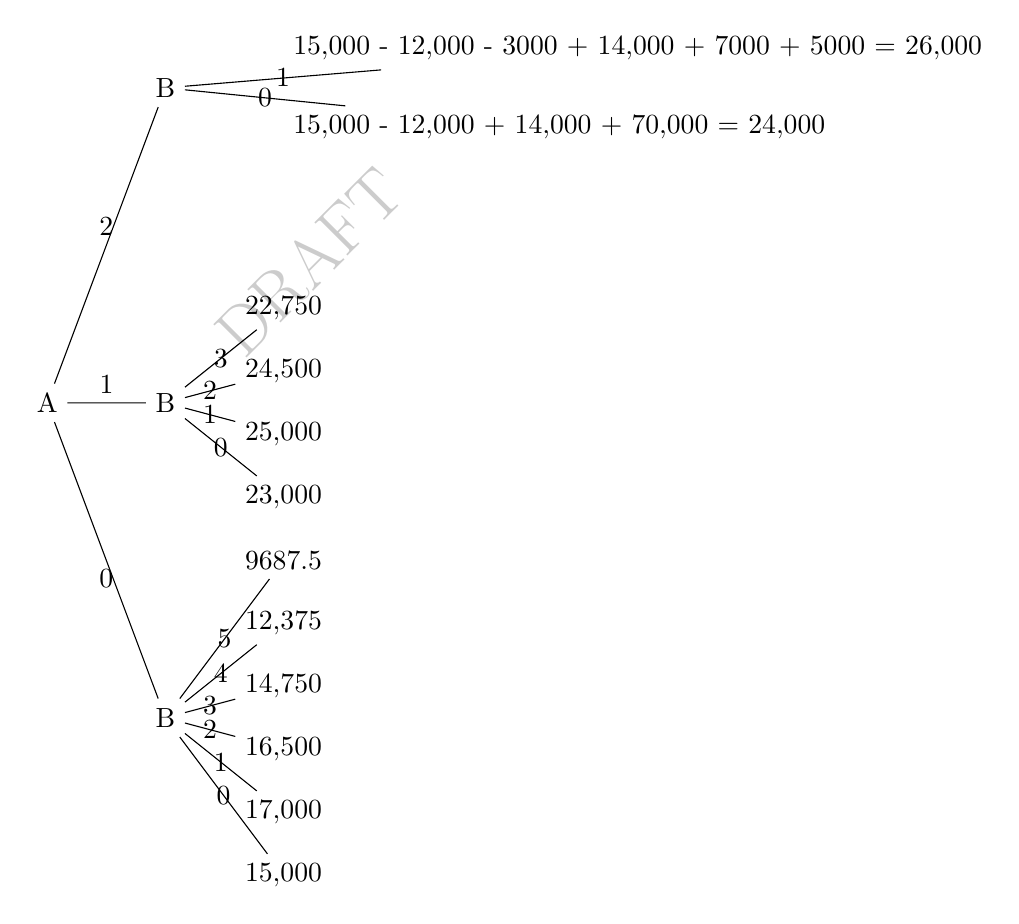
\begin{tikzpicture}
  \tikzstyle{level 1}=[sibling distance=40mm]
  \tikzstyle{level 2}=[sibling distance=8mm]
  \node {A} [grow=right]
  child{node {B} 
    child {node {\num{15000}}
    edge from parent node {0}}
    child {node {\num{17000}}
    edge from parent node {1}}
    child {node {\num{16500}}
    edge from parent node {2}}
    child {node {\num{14750}}
    edge from parent node {3}}
    child {node {\num{12375}}
    edge from parent node {4}}
    child {node {\num{9687.5}}
    edge from parent node {5}}
    edge from parent node[below] {0} }
  child {node {B}
    child {node {\num{23000}}
    edge from parent node {0}}
    child {node {\num{25000}}
    edge from parent node {1}}
    child {node {\num{24500}}
    edge from parent node {2}}
    child {node {\num{22750}}
    edge from parent node {3}}
    edge from parent node[above] {1} }
  child {node {B}
    child[sibling distance=10mm] {node[anchor=west] {\num{15000} -
    \num{12000} + \num{14000} + \num{70000} = \num{24000}}
    edge from parent node {0}}
    child[sibling distance=10mm] {node[anchor=west] {\num{15000} - 
    \num{12000} - \num{3000} + \num{14000} + \num{7000} + \num{5000} 
    = \num{26000}}
    edge from parent node {1}}
    edge from parent node[above] {2} }
  ;
\end{tikzpicture}

The company wants to make the most rational decision, so they
choose the action that maximizes the payoff. 
The company should spend the entire \$\num{15000} on robots for 
their warehouse. They should purchase two of Robot A and one of 
Robot B for a money-equivalent value of \$\num{26000}.

\end{solution}

% This exercise is OK
\item \emph{Rules for decision--making under ignorance.}
  You have the opportunity to go on a
  blind date, but you are hesitant.  You are lonely and would like to
  find the love of your life; however, you dislike awkward
  situations. Furthermore, you find it difficult to estimate the
  probability that this particular blind date will turn out to be the
  love of your life, but you know this probability is
  non-negligible. To be a little more precise, you have the following
  values: finding the love of your life is worth 1000, being in an
  awkward date situation (i.e. being on a date and knowing that you
  will not see the person again) is worth -10, and staying home
  watching Netflix is worth zero.

\begin{enumerate}
\item Formulate a decision problem for deciding whether to go on the
blind date or to stay home.
\item Use the maximin rule to solve the problem.
\item Use the minimax regret rule to solve the problem.
\end{enumerate}

\begin{solution}
\bs The decision problem can be represented with the following table.
\\[.1in]
\begin{tabular}{ccc}
 \multicolumn{3}{c}{decision matrix} \\
 & find love & lots of awkward moments \\ \cline{2-3}
go on date & 1000 & -10 \\
decline date & 0 & 0 
\end{tabular}
\\[.1in] 
The maximin rule tells you to decline the date because it has
the best of all the worst possible outcomes. To use minimax regret, we
form the regret matrix.  \\[.1in]
\begin{tabular}{ccc}
 \multicolumn{3}{c}{regret matrix} \\
 & find love & lots of awkward moments \\ \cline{2-3}
go on date & 0 & -10 \\
decline date & -1000 & 0
\end{tabular}
\\[.1in] Minimax regret tells you to go on the date because the
possibility of not finding love has the most regret.
\end{solution}


\subsubsection*{Games Against Nature}

% written by Emily
\item \emph{Gardening against nature.} A family is considering growing
  their own garden to save money on fresh vegetables. They have space
  in their yard for the garden but would need to purchase seeds and
  gardening supplies. The family is excited to grow a garden, but they
  know there are a lot of hungry rabbits in their neighborhood that
  might eat their plants before the family can harvest any vegetables
  from them. Money saved by the garden is shown in the following
  table.

\begin{tabular}{rcc}
& \multicolumn{2}{c}{State of Nature} \\
& $s_1$ & $s_2$ \\
& rabbits leave garden alone & rabbits eat garden \\ \cline{2-3}
plant garden & \$400 & -\$100\\
buy vegetables from store & 0 & 0
\end{tabular}

\begin{enumerate}
    \item If the probability that the rabbits leave the garden alone is 0.3, what decision is recommended for the family? What are the expected savings?
    
    \item The family has the option to purchase fast-growing plant seeds (the fast-growing seeds are the same price as regular seeds but they must buy the fast-growing seeds now if they want them because they are in high demand).  With these fast-growing seeds, the family can wait three more weeks to plant their garden. During that time, some scientists will finish their study on the appetites of the local rabbits, and the family will have a better idea about the probability that their garden is eaten by rabbits. They can return the seeds later for a partial refund if they do not use them.
    Let $L$ represent the event the rabbits have large appetites and let $S$ represent
    the event that rabbits have small appetites. Then
    \[
    \begin{matrix}
    P(L)=0.60, & P(s_1 \mid L)=0.15, & P(s_2 \mid L)=0.85,\\
    P(S)=0.40, & P(s_1 \mid S)=0.79, & P(s_2 \mid S)=0.21.
    \end{matrix}
    \]
    What is the optimal decision strategy if the family purchases the fast-growing seeds so they can wait and learn more about the rabbit appetites before making a decision?
    
    \item If \$40\ of the fast-growing seed purchase is non-refundable, should the family purchase the fast-growing seeds? Why or why not? What is the maximum non-refundable amount the family should pay to get the fast-growing seeds?
\end{enumerate}

\begin{solution}
\bs For part a), the expected savings when planting the garden are
\[ 400 \times 0.3  - 100 \times 0.7 = \$50. \]
The savings from not planting the garden are \$0, so based on expected value,
the best decision is to plant the garden.

For part b), if the rabbits have large appetites ($L$), then planting 
the garden would result in -\$25 of expected savings.
If the rabbits have small appetites ($S$), then planting the garden will result in \$295 
of expected savings. 

If L, \[ \$100 \times 0.15 - \$100 \times 0.85 = -\$25 \]
If S, \[ \$400 \times 0.79 - \$100 \times 0.21 = \$295 \]

Not planting will always result in \$0 of savings. 
The optimal decision strategy is to plant the garden if $S$ and buy vegetables 
from the store if $L$.

For part c), we use the optimal decision for each possible event $L$ and $S$. 
The expected savings from purchasing the fast-growing seeds
(but before actually purchasing the seeds) are
\[ \$0 \times 0.60 + \$295 \times 0.40 = \$118 \]
The maximum non-refundable amount that the family should be willing 
to pay for the fast-growing seeds is
\[ \$118 - \$50 = \$68 \]
\end{solution}

% this problem is OK
\item \emph{Using Baye's formula to update a prior belief.}
Curling is a sport in which players slide a stone over ice toward a
target. The association governing the sport has implemented drug
testing. It is believed that 15\% of all curlers use banned drugs to
enhance performance. If a player uses banned drugs, the association
may take away any prizes that the player has won; however, it
undesirable to falsely accuse someone of using banned substances.  The
utilities for each decision and state of nature are

\begin{center}
\begin{tabular}{rrrr}
& drug use & no drug use \\ \cline{2-3}
take away prizes & -100 & -1000 \\
do not & -600 & 0 
\end{tabular}
\end{center}

Notice that there is a small dis-utility for taking prizes away from a drug user
due to bad publicity for the sport. The test to detect drug use is
less than 100\% reliable. In particular, if $D$ indicates that a 
player uses banned drugs, and $+$/$-$ indicate a positive/negative
test result, then the true positive rate and the true negative rate
are
\[
P(+ \mid D) = .97 \quad \text{and} \quad P(- \mid \overline{D}) = .97,
\]
respectively, Given the utilities and the accuracy of the test, what is the best
decision if a player has a positive test result? (The association
wants to maximize expected utility.)

\begin{solution}
\bs First we update the probability of drug use via Baye's formula.
\begin{align*}
P(D \mid +) &= \frac{P(D \cap +)}{P(+)} \\
&= \frac{P(+ \mid D)P(D)}{P(+ \mid D)P(D) + P(+ \mid \overline{D})P(\overline{D})} \\
&= \frac{.97 \times .15}{.97 \times .15 + .03 \times .85} \\
&= .851
\end{align*}
and then we can compute $P(\overline{D} \mid +) = 1 - P(D \mid +) = .149$.
Using these posterior probabilities, the expected utilities are
\begin{align*}
E(\text{take away}) &= (-100)(.851) + (-1000)(.149) = -234 \\
E(\text{do not}) &= (-600)(.851) = -511
\end{align*}
The best decision is to take away prizes when a player tests positive.
\end{solution}

% Emily - expected value and sensitivity analysis
\item \emph {Decisions under risk and sensitivity analysis.}  The
  owners of a popular outdoor furniture company predict that their
  sales will double this coming year. The company is already producing
  the maximum amount of furniture possible in their current
  facility. They are considering expanding their manufacturing
  facility to accommodate the predicted increase in demand. If
  undertaken, the expansion will cost \$\num{500000}. If the demand
  doubles as predicted, revenue will increase by \$\num{800000}.  If
  the predicted increase in demand proves to be too optimistic,
  revenue will increase by only \$\num{250000}.  If the expansion is
  not undertaken, the company will lose \$\num{50000} due to
  out-of-stock orders from agitated customers.  The change in demand
  will be determined by next year's weather; more outdoor furniture is
  sold when the weather is nice.  There is a 0.55 chance of good
  weather, which will result in a doubling of demand. There is a 0.45
  chance of poor weather, which will result in only a slight increase
  in demand.

\begin{enumerate}
\item Should the manufacturing facility be expanded? The owners make
  decisions based on expected value.
\item How does the decision change with the probability of good/poor
  weather? To answer this question, you should perform a sensitivity
  analysis.
\end{enumerate}

\begin{solution}
\bs The decision table for this problem is
\begin{center}
\begin{tabular}{rrr}
      & $0.55$ & $0.45$ \\
      & good weather & poor weather \\ \hline
      expansion & \$\num{300000} & -\$\num{250000} \\
      no expansion & -\$\num{50000} & -\$\num{50000}
\end{tabular}
\end{center}

The expected payoff of each decision is
\begin{align*}
&E(\text{expansion}) = 0.55 \times \$\num{300000}
- 0.45 \times \$\num{250000} = \$\num{52500} \\
&E(\text{no expansion}) = -\$\num{50000}
\end{align*}
The company should expand the facility. As the probability of poor
weather increases, the expected value of the expansion
decreases.  Let $p$ represent the probability of poor weather.
\begin{align*}
E(\text{expansion}) &= \num{300000}(1-p) - \num{250000}p \\
&= \num{300000} - \num{550000}p
\end{align*}
The company should expand the facility as long as
\begin{align*}
E(\text{expansion}) &\geq E(\text{no expansion}) \\
\num{300000} - \num{550000}p &\geq -\num{50000} \\
-\num{5500000}p &\geq -\num{350000} \\
p &\leq \frac{7}{11} \approx .64
\end{align*}
Expanding the facility is the best decision unless the probability of
poor weather is greater than .64.
\end{solution}

\item \emph{The value of perfect information.}  You are taking a 
  date to a movie. You like horror movies but you are unsure whether
  your date likes them. You have two choices for the movie, ``The
  Burrowers'' which, despite its title, you've heard is a good movie,
  and ``A Star is Born'', which is rather safe as far as date movies
  go. Your decision problem with associated payoffs is

\begingroup
\setlength{\tabcolsep}{9pt}
\renewcommand*{\arraystretch}{2}
\begin{tabularx}{4in}{YYY}
& \multicolumn{2}{c}{Your date} \\
& likes horror movies & hates horror movies\\ \cline{2-3}
\gtcol{The Burrowers} & \gtcol{10} & \gtcol{1} \\ \cline{2-3}
\gtcol{A Star is Born} & \gtcol{4} & \gtcol{7} \\ \cline{2-3}
\end{tabularx}
\endgroup

\vspace{.2in}
\begin{enumerate}
\item Let $p$ represent the probability that your date likes horror movies. What is
  the optimal decision as a function of $p$?
\item At this point you have no information for your date's movie
  preference (even the trail of social media cannot help you) and so
  you assign $p=1/2$ as your subjective prior probability. Suppose
  that the date's best friend will tell you for sure whether your date
  likes horror movies, but this person is not so nice and wants to be
  paid. If the payoffs represent dollar amounts then how much are you
  willing to pay this person for perfect information? \label{ex:pi}
\end{enumerate}

\begin{solution}
  \bs Choose ``The Burrowers'' if
  \begin{align*}
    10p + (1-p) &> 4p + 7(1-p)\\
    9p + 1 &> -3p + 7\\
    12p &> 6\\
    p &> 1/2
  \end{align*}

  Regarding part \ref{ex:pi}, if you knew that your date liked horror
  movies you would choose ``The Burrowers'' for a pyoff of \$10 and if
  you knew the opposite then you would choose ``A Star is Born'' for a
  payoff of \$7. The expected payoff with perfect information, that
  is, before you actually receive the information, is
  \[ \frac{1}{2}(10) + \frac{1}{2}(7) = 8\frac{1}{2} \]
  Without the information your expected payoff is $\$5 \frac{1}{2}$ (for either
  choice). You would be willing to pay at most
  \[ \$8.50 - \$5.50 = \$3 \]
  for the perfect information.

\end{solution}

% written by Emily
\item \emph{Quality control and the value of perfect information.}  A
  worker in a factory producing potato chips notices that a small bolt
  is missing off of a piece of equipment in the packaging area and
  determines that it fell into a bag before it was sealed. Two pallets
  worth of chips have been produced since the last routine check was
  performed determining that the bolt was in place. The worker does
  not want to throw away all bags of chips that the bolt could
  possibly be in, so he decides to search for the bolt. He has to
  decide if he should start searching bags on pallet one or pallet
  two. If the bolt fell into a bag on pallet one and he searches bags
  on pallet one, the probability of finding the bolt by the end of the
  day is 0.5. If the bolt fell into a bag on pallet two and he
  searches pallet two, the probability of finding the bolt by the end
  of the day is 0.8. The worker's prior probability that the bolt is
  in a bag on pallet one is 0.7 (he thinks it was loose from some work
  done earlier in the day and fell off right away).

\begin{enumerate}
\item The worker only has time to search one pallet per day.  In which
  pallet, one or two, should he look for the bolt?  The worker wants
  to maximize his probability of finding the bolt.
\item Suppose that at the end of the day when the worker goes home, he
  has not found the bolt yet. Which pallet should he search on day 2?
  \emph{Hint}: First update the prior probabilities that the bolt is
  in pallet one/two.
\item Suppose that on the second day, just before the worker begins to
  search for the bolt, a security guard approaches and tells him that
  he has access to security camera footage that would reveal when the
  bolt fell into a bag (revealing which pallet the bolt is in).  How
  much should the worker be willing to pay for this perfect
  information?  Note that the ``units'' for the payment are in terms
  of probabilities.
\end{enumerate}

\begin{solution}
  \bs Let $A$ be the event that the bolt is in pallet one and let $B$
  be the event that the bolt is in pallet two. Also, let $F_A$
  represent the event that the worker finds the bolt in pallet one
  (and similarly define $F_B$). We are given the following.
\begin{align*}
  P(F_A \mid A) = 0.5 &\qquad P(\overline{F}_A \mid A) = 0.5 \\
  P(F_B \mid B) = 0.8 &\qquad P(\overline{F}_B \mid B) = 0.2 \\
\end{align*}

The worker's decision problem is

\begingroup
\setlength{\tabcolsep}{9pt}
\renewcommand*{\arraystretch}{2}
\begin{tabularx}{3.25in}{YYYY}
& & \multicolumn{2}{c}{Nature} \\
& & $0.7$ & $0.3$ \\
& & $A$ & $B$  \\ \cline{3-4}
\multirow{2}{.9in}{Worker} & \gtcol{Look in A} & \gtcol{.5} & \gtcol{0} \\ \cline{3-4}
& \gtcol{Look in B} & \gtcol{0} & \gtcol{.8} \\ \cline{3-4}
\end{tabularx}
\endgroup
\vspace{.2in}

The best option is to look in pallet one. He will find the bolt on the first
day with probability $0.7 \times 0.5 = 0.35$.

On the second day, the worker's belief that the bolt is in pallet one is updated to
\begin{align*}
  P(A \mid \overline{F}_A) &= \frac{P(\overline{F}_A \mid A)P(A)}{P(\overline{F}_A \mid A)P(A) + P(\overline{F}_A \mid B)P(B)}\\
                           &= \frac{0.5 \times 0.7}{0.5 \times 0.7 + 1 \times 0.3} \\
                           &= 0.538
\end{align*}
which implies that $P(B \mid \overline{F}_A) = 1 - 0.538 = 0.462$. On day two,
the worker's decision problem is

\begingroup
\setlength{\tabcolsep}{9pt}
\renewcommand*{\arraystretch}{2}
\begin{tabularx}{3.25in}{YYYY}
& & \multicolumn{2}{c}{Nature} \\
& & $0.538$ & $0.462$ \\
& & $A$ & $B$  \\ \cline{3-4}
\multirow{2}{.9in}{Worker} & \gtcol{Look in A} & \gtcol{.5} & \gtcol{0} \\ \cline{3-4}
& \gtcol{Look in B} & \gtcol{0} & \gtcol{.8} \\ \cline{3-4}
\end{tabularx}
\endgroup
\vspace{.2in}

and his best option is to look in pallet two. The worker will find the bolt with probability
\[ 0.462 \times 0.8 = 0.37\]

With perfect information, but \emph{before} receiving the information, the worker's
expected value for the probability of finding the bolt is
\[ 0.5 \times 0.538 + 0.8 \times 0.462 = 0.639 \]
and in terms of probability ``units'', he should be willing to pay
\[ 0.639 - 0.37 = 0.269 \]
for the information.

\end{solution}


% this problem is OK.
\item \emph{Planting crops and the value of imperfect information.} A
  farmer can plant one of four crops. The yield in bushels per acre
  depends on the particular crop planted and the weather during the
  growing season. Regarding crop yields, the weather can be
  categorized as dry, moderate, or wet. The estimated crop yields,
  commodity prices, and weather forecast are provided in the table
  below.

\begin{center}
\begin{tabular}{lcccc}
& dry & moderate & wet & \$/bushel \\ \hline
crop 1 & 30 & 50 & 60 & \$3.00 \\
crop 2 & 25 & 30 & 40 & \$4.50 \\
crop 3 & 40 & 35 & 35 & \$3.00 \\
crop 4 & 60 & 60 & 60 & \$1.50 \\ \hline
forecast & .2 & .5 & .3 & 
\end{tabular}
\end{center}

\begin{enumerate}
\item If the farmer maximizes expected monetary value, which crop
should she plant and what is her expected revenue per acre?

\item Suppose that the farmer could pay an oracle to tell her
with certainty which category of weather would occur during
the growing season. How much should the farmer be willing to 
pay for this perfect information? Your answer should be in terms
of \$/acre. \label{b}

\item Now suppose a start-up company that specializes in predictive
  modeling announces a new machine learning algorithm for weather
  forecasting. The predictions from the model are good, but not
  perfect.  In particular, the company advertises the following
  accuracy for the weather forecasting model. \label{c}

\begin{center}
\begin{tabular}{clccc}
& & \multicolumn{3}{c}{actual} \\
& & dry & moderate & wet \\ \cline{2-5}
\parbox[t]{2mm}{\multirow{3}{*}{\rotatebox[origin=c]{90}{model}}} & dry & .9 & .1 & .05 \\
& moderate & .05 & .8 & .05 \\
& wet & .05 & .1 & .9 
\end{tabular}
\end{center}

For example, if the weather actually turns out to be dry, the model
would have predicted dry weather with probability .9, moderate weather
with probability .05, and wet weather with probability .05. How much
should the farmer be willing to pay (again in \$/acre) for this
less-than-perfect prediction of the weather? Settle in with a cup of
coffee: this part requires some work. Here is a strategy.
\begin{enumerate}[i)]
\item Develop a notation, e.g., $x$ indicates the weather during the growing season,
and $x'$ indicates the prediction, where $x$ is dry, moderate, or wet.

\item Use Baye's formula to compute the posterior probabilities for
  each weather category given the predictions, e.g. you want to know
  $P(d \mid d')$, $P(m \mid d')$, etc.

\item Determine the expected payoff for each case that the prediction is
dry, moderate, and wet.

\item The expected value of the prediction (i.e. the expected value of the
less-than-perfect information) is the difference between the expected payoff
with the information and without it.
\end{enumerate}

\end{enumerate}

\begin{solution}
\bs Considering the estimated commodity prices, the payoff table and expected
values in \$/acre for each crop are

\begin{center}
\begin{tabular}{lrrrr}
& dry & moderate & wet & $E(\text{payoff})$ \\ \hline
crop 1 & 90 & 150 & 180 & \$147 \\
crop 2 & 112.5 & 135 & 180 & \$144 \\
crop 3 & 120 & 105 & 105 & \$108 \\
crop 4 & 90 & 90 & 90 & \$90 
\end{tabular}
\end{center}

To maximize expected monetary value the farmer should plant crop 1 and
expect \$147/acre of revenue. For part~\ref{b}, if she knew for
certain that the weather would be dry, moderate, or wet, then she
would plant crop 3 with revenue \$120 per acre, crop 1 with revenue
\$150 per acre, and crop 1 (or 2) with revenue \$180 per acre,
respectively. Prior to learning the perfect information, the farmer's
expected payoff with the new information is
\[
.2 \times \$120 + .5 \times \$150 + .3 \times \$180 = \$153
\]
and so the value of the perfect information is worth no more than
\[
\$153 - \$147 = \$6~\text{per acre}
\]

Now for part~\ref{c}, the likelihoods are provided as follows
(using the notation given in the problem description).
\[
\begin{matrix}
P(d' \mid d)=.9 & P(m' \mid d)=.05 & P(w' \mid d)=.05 \\
P(d' \mid m)=.1 & P(m' \mid m)=.8 & P(w' \mid m)=.1 \\
P(d' \mid w)=.05 & P(m' \mid w)=.05 & P(w' \mid w)=.9 \\
\end{matrix}
\]

Using Baye's formula to compute the posterior probabilities, we get
\begin{align*}
P(d \mid d') &= \frac{P(d \cap d')}{P(d')} \\
&= \frac{P(d' \mid d)P(d)}{P(d' \mid d)P(d) + P(d' \mid m)P(m) + P(d' \mid w)P(w)} \\
&= \frac{(.9)(.2)}{(.9)(.2) + (.1)(.5) + (.05)(.3)} \\
&= .735
\end{align*}
and in a similar manner 
\[
\begin{matrix}
& P(m \mid d')=.204 & P(w \mid d')=.061 \\
P(d \mid m')=.024 & P(m \mid m')=.941 & P(w \mid m')=.035 \\
P(d \mid w')=.03 & P(m \mid w')=.152 & P(w \mid w')=.818 \\
\end{matrix}
\]
The expected monetary values given the predictions are

\begin{center}
\begin{tabular}{lrrr}
& $E(\text{dry})$ & $E(\text{moderate})$ & $E(\text{wet})$ \\ \hline
crop 1 & \$108 & 150 & 173 \\
crop 2 & 121 & 136 & 171 \\
crop 3 & 116 & 105 & 105 \\
crop 4 & 90 & 90 & 90
\end{tabular}
\end{center}

If the prediction is dry, the farmer would plant crop 2 for an
expected revenue of \$121 per acre. Similarly for predictions
of moderate and wet, she would plant crop 1 with expected revenue
\$150 per acre and crop 1 with expected revenue \$173 per acre,
respectively. Prior to obtaining the weather prediction,
the expected value of having the prediction is 
\begin{align*}
E(\text{payoff}) &= \$121 \times P(d') + \$150 \times P(m') + \$173 \times P(w') \\
&= \$121 \times .245 + \$150 \times .425 + \$173 \times .33 \\
&= \$150.50
\end{align*}
Note that the unconditional probabilities of the predictions are obtained
using the formula for total probability and they were computed during the
application of Baye's formula. The value of the less-than-perfect
informtaion is 
\[
\$150.50 - \$147 = \$3.50~\text{per acre}
\]
\end{solution}

% decisions over time
% this problem is OK.
\item \emph{The break-up.} You are considering
  breaking up with your boy(girl)friend; however, you know that
  he(she) may break up with you. Your utility is higher if you end
  the realtionship, but it's Friday and you have joint plans for the
  weekend. Here is the situation: on Friday (and possibly Saturday)
  you need to decide to either stay in the relationship, or end it.
  \begin{compactitem}[i)]
    \item \emph{On Friday:}
  If you decide to end the relationship your payoff is one
  (and your done.) If you stay in the relationship then a random
  chance event happens where your boy(girl)friend ends the relationship
  with probability 0.25 and stays with probability 0.75.
\item \emph{On Saturday:} If you end the relationship your
  payoff is 3 (and your done.) If you stay then a chance event happens
  where your boy(girl)friend ends the relationship with probability
  0.5 and stays with probability 0.5.
\end{compactitem}
If you stay in the relationship until Sunday, then you will definitely
end it and your payoff is 4. If, on Friday or Saturday, your boy(girl)friend
ends the relationship then your payoff is one.

Use backward induction to determine a policy for ending/staying that
will maximize your expected payoff.

\begin{solution}
  \bs The decision tree is shown below. Working backwards, the expected
  value of ``stay'' on Saturday is 2.5, so the best decision is ``exit'',
  for a payoff of 3. On Friday, the expected value of ``stay'' is 2.5,
  which is better than ``exit'' with a payoff of 1. So, the policy that
  maximizes expected payoff is to stay in the relationship on Friday and
  exit the relationship on Saturday.

\vspace{.2in}
\begin{center}
%\resizebox{.5\textwidth}{!}{%
  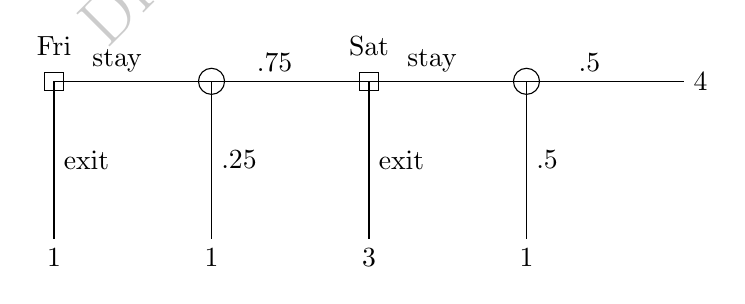
\begin{tikzpicture}
    \draw (0,0) -- (8,0)
    node[pos=.1,anchor=south] {stay}
    node[pos=.35,anchor=south] {.75}
    node[pos=0.6,anchor=south] {stay}
    node[pos=.85,anchor=south] {.5}
    node[right] {4};
    \draw (0,0) -- (0,-2) node[pos=0.5,anchor=west] {exit} node[below] {1};
    \draw (2,0) -- (2,-2) node[pos=.5,anchor=west] {.25} node[below] {1};
    \draw (4,0) -- (4,-2) node[pos=0.5,anchor=west] {exit} node[below] {3};
    \draw (6,0) -- (6,-2) node[pos=0.5,anchor=west] {.5} node[below] {1};
    \node[draw] at (0,0) {};
    \node[circle,draw] at (2,0) {};
    \node[draw] at (4,0) {};
    \node[circle,draw] at (6,0) {};
    \node[anchor=south] at (0,0.2) {Fri};
    \node[anchor=south] at (4,0.2) {Sat};
\end{tikzpicture}%}
\end{center}
\end{solution}

% this problem needs a different context.
% the idea is to use backward induction to find an optimal policy.
\item \emph{An optimal strategy for a chess match.}  Alice is
  preparing for a two--game chess match.  In each game Alice can
  choose one of two strategies: timid play or bold play. The strategy
  selected in the second game can differ from the strategy selected
  in the first game. If Alice plays bold then she will win with
  probability $p_w$ and lose with probability $1-p_w$. If Alice
  chooses timid play then the match will result in a draw with probability
  $p_d$ and she will lose the match with probability $1-p_d$. Note
  that bold play results in a either a win or a loss, and that timid
  play results in either a draw or a loss. At the conclusion of each
  game, each player is awarded 1 point for a win, 1/2 point for a
  draw, or zero points for a loss. If the score is tied at the of two
  games, then the match goes into sudden death and the first person to
  win a game wins the match.  Let $p_w=0.45$ and let $p_d=0.9$. Which
  strategy should Alice select for the first game of the match, timid
  or bold? What about the second game? In other words, what is the
  strategy that will maximize Alice's expected payoff for the match?

  Note that the payoff for Alice is the difference in scores. For
  example, suppose that Alice plays timid in the first game resulting
  in a draw and she plays bold in the second game resulting in a win.
  Then the score for the match is Alice $1\frac{1}{2}$ points and her
  opponent $\frac{1}{2}$ point. In that case the payoff for Alice is
  $1\frac{1}{2} - \frac{1}{2} = 1$. Also consider that in the event of
  a tied score at the end of two games Alice should play bold in
  sudden death.  If she plays timid during sudden death then the best
  that she could hope for is to drag out the match indefinitely. The
  payoff for Alice for a tied score after two games is the expected
  value of a lottery wherein she gets 1 point with probability $p_w$
  and -1 point with probability $1-p_w$.

\begin{solution}
  \bs The optimal strategy for Alice, i.e. the strategy that maximizes
  her expected payoff is to play timid in the first game. If she loses
  the first game then play timid in the second game, otherwise if she
  draws in the first game, then play bold in the second game.  Please
  see the attached decision tree. 
\end{solution}

\subsubsection*{Games Against an Opponent}

% written by Emily
\item \emph{Elimination of dominated strategies.}
Two street vendors, A and B, are located near a major tourist attraction. 
The proportion of customers
captured by each vendor depends on the merchandise sold by that vendor and by
her competitor. A customer gained by one is lost to the other. Each vendor
can stock one of the following: clothing, ice cream, or souvenirs.
The possible strategies and proportion of customers captured are as follows.

\begin{tabular}{l}
If both shops sell souvenirs, A captures 75\% of the customers.\\
If both shops sell clothing, A and B split the customers evenly.\\
If both shops sell ice cream, A and B split the customers evenly.\\
If B sells ice cream and A sells souvenirs, A captures 10\%.\\
If B sells clothing and A sells ice cream, A captures 90\%.\\
If B sells souvenirs and A sells clothing, A captures 10\%.\\
If A sells clothing and B sells ice cream, A captures 100\%.\\
If A sells souvenirs and B sells clothing, A captures 75\%.\\
If A sells ice cream and B sells souvenirs, A captures 40\%.
\end{tabular}

\setlength{\parindent}{0cm}
Model the decision of each vendor as two-person zero-sum game
and find a solution by elimination of dominated strategies.

\begin{solution}
\bs The game is

\begingroup
\setlength{\tabcolsep}{9pt}
\renewcommand*{\arraystretch}{2}
\begin{tabularx}{4.5in}{YYYYY}
& & \multicolumn{3}{c}{B} \\
& & clothing & ice cream & souvenirs \\ \cline{3-5}
\multirow{3}{.25in}{A} & \gtcol{clothing} & \gtcol{.50} & \gtcol{1} & \gtcol{.10} \\ \cline{3-5}
& \gtcol{ice cream} & \gtcol{.90} & \gtcol{.50} & \gtcol{.40} \\ \cline{3-5}
& \gtcol{souvenirs} & \gtcol{.75} & \gtcol{.10} & \gtcol{.25} \\ \cline{3-5}
\end{tabularx}
\endgroup
\vspace{.1in}

For A, ice cream strictly dominates souvenirs and for B, souvenirs
strictly dominates clothing, leaving a $2 \times 2$ game.

\begingroup
\setlength{\tabcolsep}{9pt}
\renewcommand*{\arraystretch}{2}
\begin{tabularx}{4in}{YYYY}
& & \multicolumn{2}{c}{B} \\
& & ice cream & souvenirs \\ \cline{3-4}
\multirow{2}{.25in}{A} & \gtcol{clothing} & \gtcol{1} & \gtcol{.10} \\ \cline{3-4}
& \gtcol{ice cream} & \gtcol{.50} & \gtcol{.40} \\ \cline{3-4}
\end{tabularx}
\endgroup
\vspace{.1in}

Now for B, souvenirs dominates ice cream. Then, A will choose to sell
ice cream over clothing. So, the best strategies for A and B are to
sell ice cream and souvenirs, respectively.  Using this pair of
strategies, A will capture 40\% of the customers.
\end{solution}

% written by Emily to replace Goldsen and Kershaw battle of words
\item \emph{A two-person zero-sum game.}  A professional football
  player believes that the team he plays for should be allocating more
  money to the salaries of the players, so he wants his contract to be
  changed to pay him more. His two options are to play in the upcoming
  season or not play in the upcoming season and hope the team will
  negotiate with him. The team knows that he is a valuable player but
  does not want to pay him more or go through the process of
  negotiations. The team has come up with three options to deal with
  the situation: negotiate, refuse to negotiate and play the season
  without him, or increase the player's salary by a set amount with no
  other negotiations. Keep in mind that the player wants to maximize
  his salary, and the team wants to minimize their costs, which means
  keep salaries as low as possible. The utilities/payoffs to
  the player and to the team are described next.

  If the player plays and the team does not negotiate, the player's
  salary will not change.  If the player does not play and the team
  does not negotiate, the player will find a different job as a
  broadcaster for a payoff of 1 because he is such a well-known
  person. This is bad publicity for the team and hurts their jersey
  sales.  If the player plays but the team still negotiates, the
  player will end up with a payoff of 3.  If the player had
  chosen to not play and the team negotiates, the negotiations will go
  poorly and the player will end up with a payoff of -2 for having to
  deal with costs related to poor publicity.  If the team decides
  increase the player's salary with no negotiations, the player will
  end up with a payoff of 2 no matter what he chooses to do.


  Formulate the 2-by-3 game and determine the best strategy for the
  player and for the team.  Who is most likely to come out ahead in
  this situation?
  
\begin{solution}
\bs The game is

\begingroup
\setlength{\tabcolsep}{9pt}
\renewcommand*{\arraystretch}{2}
\begin{tabularx}{4.5in}{YYYYY}
& & \multicolumn{3}{c}{Team} \\
& & negotiate & don't negotiate & increase salary \\ \cline{3-5}
\multirow{2}{.5in}{Player} & \gtcol{play} & \gtcol{3} & \gtcol{0} & \gtcol{2} \\ \cline{3-5}
& \gtcol{don't play} & \gtcol{-2} & \gtcol{1} & \gtcol{2} \\ \cline{3-5}
\end{tabularx}
\endgroup
\vspace{.1in}

The team's strategy of a set
increase is dominated by the strategy to not negotiate, so there is no
reason that they would chose to offer a pre-determined
increase without negotiations. The reduced game is

\begingroup
\setlength{\tabcolsep}{9pt}
\renewcommand*{\arraystretch}{2}
\begin{tabularx}{4in}{YYYY}
      & & \multicolumn{2}{c}{Team} \\
      & & {negotiate} & {don't negotiate} \\ \cline{3-4}
      \multirow{2}{.5in}{Player} & \gtcol{play} & \gtcol{3} & \gtcol{0} \\ \cline{3-4}
      & \gtcol{don't play} & \gtcol{-2} & \gtcol{1} \\ \cline{3-4}
\end{tabularx}
\vspace{.1in}
\endgroup

Since there is no saddle point, the best strategies for the player and
for team are mixed. The player should mix the strategies ``play'' and
``don't play'' in the ratio 1:1. The team should mix the strategies
``negotiate'' and ``don't negotiate'' in the ratio 1:5.  Using the
player's mixing ratios against the team's strategy of ``negotiate''
the value of the game is computed as
\[
\frac{1 \times (3) + 1 \times (-2)}{2} = 1/2.
\]
The player is more likely to come out ahead. 
\end{solution}
  
% written by Emily to replace cops and robbers
\item \emph{Marketing strategies.} Two peanut butter companies,
  Doodle's and Lola's, are deciding on their marketing strategy for
  the upcoming year. They know that they are each other's main
  competitor and that the demand for peanut butter is relatively
  constant, so a gain in sales for Doodle's is a loss of sales for
  Lola's. Each company has their standard packaging for peanut butter
  and a new innovative packaging for peanut butter. Both companies
  may produce and sell both types of packaging.  If both
  companies choose to market only their innovative packaging, Doodle's
  will gain an extra 2\%\ of the market's sales.  If both companies
  choose to market their standard packaging, Doodle's will loose 2\%\
  of the market.  If Doodle's markets their innovative product and
  Lola's markets their standard product, Doodle's will gain 10\%\
  of the market.  If Lola's markets their innovative product and
  Doodle's markets their standard product, Doodle's will gain 8\%\
  of the market.
 
\begin{enumerate}
\item Formulate this decision problem as a two-person zero-sum game
  and determine the optimal marketing strategy for each company. Note
  that they are able to change their advertising throughout the year,
  so a mixed strategy is possible.
\item Compute the value of the game. \label{val}
\item Suppose that a member of Doodle's marketing team quits her
  job and goes to work for Lola's. She tells her new co-workers
  about the strategy that Doodle's is planning to use. She is even able to
  tell them the probabiliites with which Doodle's will market their
  standard product and their innovative product. Lola's marketing
  team now knows that Doodles is more likely to market the innovative
  product than the standard product. Armed with this knowledge, they
  choose to only market their standard product, thinking that this
will improve their payoff. Is Lola's argument
  valid? In other words, does the value of the game change if
  Lola's knows Doodle's optimal strategy?
\label{knowledge}
\end{enumerate}

\begin{solution}
\bs The game is

\begingroup
\setlength{\tabcolsep}{9pt}
\renewcommand*{\arraystretch}{2}
\begin{tabularx}{3.25in}{YYYY}
& & \multicolumn{2}{c}{Lola's} \\
& & standard & innovative \\ \cline{3-4}
\multirow{2}{.5in}{Doodle's} & \gtcol{standard} & \gtcol{-2} & \gtcol{8} \\ \cline{3-4}
& \gtcol{innovative} & \gtcol{10} & \gtcol{2} \\ \cline{3-4}
\end{tabularx}
\endgroup
\vspace{.1in}

Note that there is no saddle point, and so the best strategy is mixed.
Doodle's should mix the strategies standard and innovative
in the ratio 4 to 5, while Lola's should mix their strategies of
standard to innovative in the ratio 1 to 2.  The corresponding
probabilities are $(4/9,\,5/9)$ for Doodle's and $(1/3,\,2/3)$ for
Lola's.

To compute the value of the game, note that when
Doodle's markets the standard product, they receive a payoff of -2
with probability 1/3 and payoff of 8 with probability 2/3.  The value
of the game is
\[ \frac{1 \times -2 + 2 \times 8}{3} = \frac{14}{3} = 4.67 \]
On average Doodle's comes out ahead.

Regarding part \ref{knowledge}), the team's thought process is not
valid.  As long as one player sticks to the optimal mixed strategy,
the value of the game does not change.
\end{solution}

% written by Emily to replace the silver dollar
\item \emph{The birthday gift.} Liam's birthday is coming up and he
  can't wait to see what he will get as a gift. Liam's parents want
  the gift to be a surprise, but they always hide gifts in either the
  kitchen or the basement. Liam plans to search for the gift when his
  parents are busy, but he knows that even if he searches the room
  that contains the gift, he may not find it. If the gift is hidden in
  the kitchen and Liam searches the kitchen, he will find the gift
  with probability 0.75.  If the gift in hidden in the basement and he
  searches the basement, then he will find it with probability 0.5.
  If he searches the wrong room, there is no way he will find the
  gift. Assume that the payoff to Liam for finding the gift early is
  the same as the payoff to the parents of keeping the gift a
  surprise.  Formulate this game as a two-person, zero-sum game. Liam
  is the row player and his parents are the column player. Find the
  optimal strategies for both players. \label{sda}

\begin{solution}
  \bs Liam has two possible actions for this game: search the kitchen
  or search the basement. His parents also have two options: hide the
  gift in the kitchen or hide the gift in the basement.  The game is

\begingroup
\setlength{\tabcolsep}{9pt}
\renewcommand*{\arraystretch}{2}
\begin{tabularx}{4in}{YYYY}
& & \multicolumn{2}{c}{Parents} \\
& & hide in kitchen & hide in basement \\ \cline{3-4}
\multirow{2}{.5in}{Liam} & \gtcol{search kitchen} & \gtcol{3/4} & \gtcol{0} \\ \cline{3-4}
& \gtcol{search basement} & \gtcol{0} & \gtcol{1/2} \\ \cline{3-4}
\end{tabularx}
\endgroup
\vspace{.1in}

and the optimal strategy is the same for both players. Each
should play a mixture of $(2/5,~3/5)$.
\end{solution}

% written by Emily
\item \emph{Workforce staffing.}  A salon is trying to decide how many
  stylists they should have available for walk-in customers. The
  hourly walk-in demand is specified by the following probability
  distribution, where $p_n$ is the probability of having $n$ customers
  in one hour.

\vspace{.2in}
\begin{tabular}{r|rrrrr}
$n$ & 1 & 2 & 3 & 4 & 5 \\ \hline
$p_n$ & .10 & .20 & .35 & .25 & .10 \\
\end{tabular}

\vspace{.2in} Each stylist costs the salon \$20\ per hour.  If a
stylist has a customer that hour, the salon will charge the customer
\$45\ for service.  Each customer requires about an hour of time from
a stylist.  If a stylist does not have a customer that hour, he/she
will complete a different task in the salon which adds \$9\ of
value. If all stylists are busy with a customer and an additional
customer arrives, that customer will be turned away and will go to a
different salon. How many stylists should be available each hour in
order to maximize profit for the salon?

\begin{solution}
  \bs Let $Q$ represent the available number of stylists (quantity)
  and let $z$ represent the demand. There are two situations.  First,
  if $Q \geq z$
\begin{align*}
E(\text{profit}) &= 45z - 20Q + 9(Q-z) \\
&= 36z - 11Q
\end{align*}
Otherwise if $Q < z$, then
\begin{align*}
E(\text{profit}) &= 45Q - 20Q\\
&= 25Q
\end{align*}

We use the distribution of demand to compute the expected profit
for each possible level of staffing.
\begin{center}
\begin{tabular}{rr|rrrrrr}
& & \multicolumn{5}{c}{$z$} & \\
& & .1 & .2 & .35 & .25 & .1 & \\
& & 1 & 2 & 3 & 4 & 5 &  $E(\text{payoff})$ \\ \hline
\multirow{5}{*}{$Q$} & 1 & 25 & 25 & 25 & 25 & 25 & 25 \\
& 2 & 14 & 50 & 50 & 50 & 50 & 46.4 \\
& 3 & 3 & 39 & 75 & 75 & 75 & 60.6 \\
& 4 & -8 & 28 & 64 & 100 & 100 & 62.2 \\
& 5 & -19 & 17 & 53 & 89 & 125 & 54.8
\end{tabular}
\end{center}

The best decision is to have 4 stylists available.
\end{solution}

\subsubsection*{Utility Theory}

% Written by Emily
% Expected Utility Theorem
\item \emph{Expected utility of a day off.}  Utilities are the basis
  for making rational decisions.  Sydney has the day off from work and
  she is trying to decide what to do. Her top three options and their
  utilities are:

\begin{tabular}{lr}
  option & utility \\ \hline
  go to the beach & 100\\
  go hiking & 75\\
  stay home and watch movies & 50
\end{tabular}

With only this information, Sydney would choose to go to the beach for
the day. However, there is some uncertainty (or risk) in Sydney's
decision. The weather and the people she runs into at the beach or
while hiking impact her utility.  Sydney does not enjoy being outside
when it is raining.  If it rains while she is at the beach, her
utility is decreased by 80.  If it rains while she is hiking, her
utility is decreased by 30.  On the other hand, Sydney enjoys running
into friends. If she runs into a friend at either the beach or on the
hiking trail, it will increase Sydney's utility by a factor of 1.5
(after any disutility has been appplied).

At the beach, it is rainy 40\% of the time and Sydney has a 30\%
chance of running into a friend.  On the hiking trail, it is rainy
20\% of the time and she has a 50\% chance of running into a friend.
Compute Sydney's expected utilities for each option. What is the
``rational'' decision for Sydney?

With this exercise, there are three points to be made:
\begin{enumerate}
\item Rational choice means that agents (like Sydney) make decisions 
    that maximize their utility (or payoff, or happiness). It doesn't 
    mean that agents only care about themselves. Agents have 
    preferences over states of the world. An agent might have a preference 
    for making another agent happy, and that would be reflected in her 
    utility for that state of the world.
\item Each agent has a utility function that maps states of the world
    to real numbers that represent the agent's level of happiness.
\item When there is uncertainty over which state will occur, then
    an agent's utility is her expected utility.
\end{enumerate}

\begin{solution}
\bs We must calculate the expected utility for each possible decision.
The expected utility of going to the beach is:
\begin{align*}
E(\text{utility}) &= 100 - 80 \times 0.40 + 
(100 - 80 \times 0.40) \times 0.50 \times 0.30 \\
&= 78.20
\end{align*}
The expected utility of going hiking is:
\begin{align*}
E(\text{utility}) &= 75 - 30 \times 0.20 + (75 - 30 \times 0.20) \times 0.50 \times 0.50 \\
&= 86.25
\end{align*}
The expected utility of staying home watching movies is 50 because it
is influenced by neither the weather nor running into friends. The
``rational'' decision for Sydney is to go hiking.
\end{solution}

\item \emph{Attitudes toward risk.}  Consider the following scenarios
  for Alice and Bob. Then, draw reasonable utility functions for each
  person. Alice's utility function should be in the range zero to
  \$100K.  Bob's should be from zero to \$40.

  Alice has worked hard to save \$25K for a down payment on a
  house. She is ready to buy the house, but just before closing, she
  is offered the following hot tip. If she invest invests \$25K in a
  cryptocurrency, there is an 80\% chance that she will make \$50K
  within one month, but a 20\% chance that she will lose everything.
  The expected monetary value of the opportunity is
  \[
  0.8 \times \$75\text{K} - 0.2 \times \$25\text{K} = \$55\text{K},
  \]
  but Alice makes the \$25K down payment even though the EMV of the
  investment is higher. The certainty of getting the house is worth
  more to her than the uncertain gain from the investment.

  Bob has \$20 in his possession. He \emph{really} wants to see the
  show at First Avenue, but tickets cost \$40. Over on 7th Street,
  someone comes along and offers Bob the following gamble.
\begin{quote}
  Put in \$20. Roll a die. If the die comes up ``6'', then the player
  wins \$20. If the die comes up any other number the player loses the
  \$20.
\end{quote}
If Bob is lucky enough to win the gamble, he would have \$40 for the
ticket. The expected monetary value of the gamble is
  \[
  \frac{1}{6} \times \$40 - \frac{5}{6} \times \$20 = -\$10,
  \]
  but Bob takes the bet because the chance to see the show is worth
  more to him than having \$20 and \emph{not} seeing the show.

\begin{solution}
  \bs The important point is the general shape of the utility
  functions, not the magnitudes of the utilities. Alice is risk-averse
  and Bob is risk-seeking.

\begin{minipage}{.49\textwidth}
\resizebox{\textwidth}{!}{%
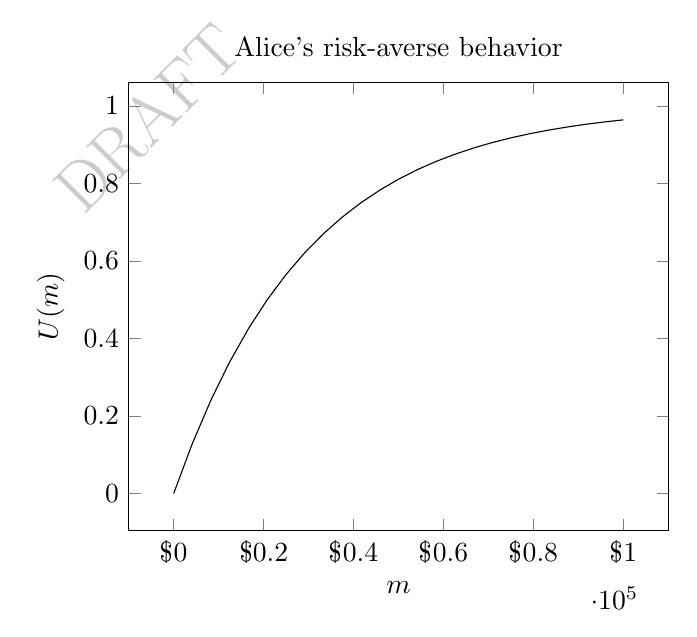
\begin{tikzpicture}
\begin{axis}[
xlabel={$m$},
ylabel={$U(m)$},
xticklabel={\$$\pgfmathprintnumber{\tick}$},
title=Alice's risk-averse behavior,
]
\addplot[domain=0:100000] {1 - exp(-x/30000)};
\end{axis}
\end{tikzpicture}}
\end{minipage}
\hfill
\begin{minipage}{.49\textwidth}
\resizebox{\textwidth}{!}{%
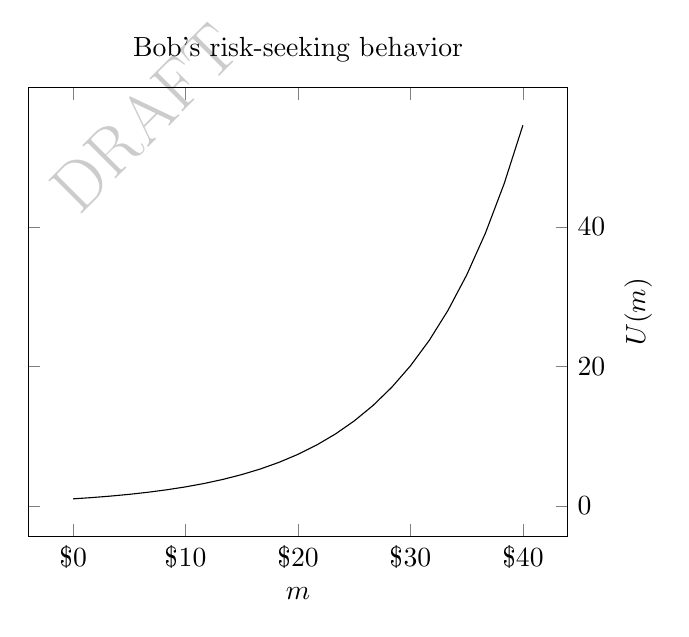
\begin{tikzpicture}
\begin{axis}[
xlabel={$m$},
ylabel={$U(m)$},
xticklabel={\$$\pgfmathprintnumber{\tick}$},
title=Bob's risk-seeking behavior,
yticklabel pos=right,
]
\addplot[domain=0:40] {exp(x/10)};
\end{axis}
\end{tikzpicture}}
\end{minipage}

\end{solution}

\item \emph{Registering for classes.} You are deciding to register for
  one of two classes, IE 5571 or IE 5591. If you register for IE 5571
  you know that you will get a B for sure, but IE 5591 is a lottery
  because the department has not yet decided who will teach the
  class. If Professor England teaches the class then you will get an
  A, but if Professor Doroudi teaches the class then you will get a
  C. You will not know the identity of the instructor until class
  begins and you cannot withdraw from the course once registered. The
  points associated with the letter grades are

\begingroup
\renewcommand{\arraystretch}{1}
\begin{tabular}{cccc}
A&B&C&D \\
4.0 & 3.0 & 2.0 & 1.0
\end{tabular}
\endgroup

Now, you value having fun as much or more than improving your GPA. In
fact, your utility for the points $x$ associated with a letter grade
is $u(x) = \sqrt{x}$. That is to say, your utility for getting a B is
$\sqrt{3}$. The ISyE department head tells you that the probability
that Professor Doroudi will teach IE 5591 is 2/5.

\begin{enumerate}
\item For which class will you register?
\item In general, what is your risk profile toward letter grades?
  (A \emph{brief} answer will suffice.)
\item Your preferences satisfy the conditions of the Expected Utility
  Theorem.  Furthermore, your utility function $u(x)$ was determined
  via questions pertaining to preferences between pairs of
  alternatives (including lotteries). Is it appropriate to say that
  receiving an A is twice as desirable as receiving a D?
\end{enumerate}

\begin{solution}
\bs
The utility of registering for IE 5571 is
\[ u(B) = \sqrt{3} \]
By the expected utility property, the utility of a lottery is its
expected utility. So the utility of registering for IE 5591 is
\begin{align*}
  u\left(L\left(\frac{3}{5},~A,~C\right)\right) &= \frac{3}{5}u(A) + \frac{2}{5}u(C) \\
                  &= \frac{3}{5}\sqrt{4} + \frac{2}{5}\sqrt{2} \\
                  &= \frac{6 + 2\sqrt{2}}{5}
\end{align*}
which is greater than $\sqrt{3}$, so you will register for IE 5591.
In general you are risk-averse with respect to letter grades. It
is \emph{not} appropriate to say that receiving an A is twice
as desirable as receiving a D. Utility functions are defined for
interval scales, not for ratio scales.

\end{solution}

% written by Emily
\item \emph{Preference orderings and utility functions.}  This
  exercise is inspired from discussion in~\cite{resnik:1987}.  Suppose
  you have a goal to be a great long-distance runner.  There are two
  choices involved with this goal in the form of $(x;y)$ where $x$
  represents the number of miles you are able to run in a day after
  you have trained for a month, anywhere from zero to 30 miles, and
  $y$ represents the total number of miles ran to train over the
  course of the month, anywhere from zero to 500. Both $x$ and $y$ are
  continuous distances, and $x \le y$. In general you prefer to be
  able to run farther with less training, but you always prefer to be
  able to run father no matter how much you have to train. For
  example,
  \[
  (x=25~\text{miles}; y=500~\text{miles}) \succ (x=24~\text{miles}; y=200~\text{miles})
  \]
  The symbol `$\succ$' means ``is preferred to''.  Don't confuse that
  symbol with the mathematical inequality symbol `$>$' (although I
  suspect that the resemblence is intended). Note that, as defined, your
  preference ordering satisfies the completeness and transitivity
  properties (see the discussion on page~\pageref{rules-of-consistency}). 
  Is it possible to represent your
  preferences with a single (real-valued) number? That is to say, is
  there a function $u(x,y) : (x,y) \mapsto \mathbb{R}$ with the
  following property
  \[
  (x_1,y_1) \succ (x_2,y_2)~\implies~u(x_1,y_1) > u(x_2,y_2)
  \]
  To make things a little easier, you can restrict $u$ to be a linear
  function of $x$ and $y$. Support your answer with an explanation
  \ldots a formal proof is great, but not required.

\begin{solution}
  \bs I think it is not possible to represent $u$ as a linear
  function of $x$ and $y$. Define $w=500-y$, so that we can represent
  an alternative as $(x,w)$ with the interpretation that more is always
  better, but $x$ still has priority. Now, a linear function will have
  the form
  \[
  u(x,w) = Ax + Bw
  \]
  where $A$ and $B$ are constants.
  It is enough to show a situation where $(x_1;w_1) \succ (x_2;w_2)$
  but that $u(x_1,w_1) < u(x_2,w_2)$. We can write $x_2=x_1-\delta_x$
  and $w_2=w_1+\delta_w$ where $\delta_x > 0$ (so that $x_1>x_2$).
  Now,
  \[
  u(x_1,w_1) = Ax_1 + Bw_1
  \]
  and
  \begin{align*}
    u(x_2,w_2) &= u(x_1-\delta_x,w_1+\delta_w) \\
    &= A(x_1-\delta_x) + B(w_1 + \delta_w) \\
    &= Ax_1 - A\delta_x + Bw_1 + B\delta_w \\
    &= Ax_1 + Bw_1 + (B\delta_w - A\delta_x)
  \end{align*}
  We need only to show that $B\delta_w-A\delta_x > 0$.
  \begin{align*}
    B\delta_w - A\delta_x &> 0 \\
    B\delta_w &> A\delta_x \\
    \frac{\delta_w}{\delta_x} &> \frac{A}{B}
  \end{align*}
  Note that $\delta_w = w_2-w_1 = y_1-y_2 \leq 500$, but because $x$
  is continuous, we can choose $\delta_x$ and $\delta_w$ to satisfy
  the last inequality, which means that $u(x_1,w_1) < u(x_2,w_2)$.
\end{solution}

\end{enumerate}
%%% Local Variables:
%%% TeX-master: "main"
%%% End:

\chapter{Data Analysis}
\label{data-analysis}

\section{Descriptive Statistics}

Point estimate of a population proportion. Consider the
  pizza delivery data that is available on the class Moodle
  page. Construct a point estimate of the probability that the amount
  of tips received in a shift is greater than \$60. What is the
  standard error of your point estimate? You can do the calculations
  by hand or use the software of your choice. If you use software, you
  can use it in any way you like.  For example, I used R as a
  calculator to simply help with the required computations.
  
\begin{Verbatim}
pizza <- read.table("pizza.txt", header=TRUE)
attach(pizza)
x <- sum(Tips > 60)
n <- length(Tips)

# follow the formula for the point estimate and the standard
# error of a sample proportion
phat <- x/n
se <- sqrt((phat*(1-phat))/n)

> phat
[1] 0.2413793
> se
[1] 0.0212373
\end{Verbatim}

% discussion of confidence interval.
% change problem context, have >= 30 observations, use Normal distribution.
  \emph{Confidence Interval.}  An article in the \emph{Journal of Heat
    Transfer} describes a method of measuring the thermal conductivity
  of high-purity iron.  Using a temperature of $100^{\circ}$F and a
  power input of 550 W. The following 10 measurements of thermal
  conductivity (in Btu/hr -- ft -- ${}^{\circ}$F) were determined.
\begin{align*}
  41.60,~41.48,~&42.34,~41.95,~41.86\\
  42.18,~41.72,~&42.26,~41.81,~42.04
\end{align*}
A point estimate of the population mean thermal conductivity
(at $100^{\circ}$F and 550 W) is the sample mean
\[
  \mean{X} = 41.924
\]
The standard error of the sample mean (i.e. the standard error
of the point estimate) is
\[
  \text{se}(\mean{X}) = \frac{S}{\sqrt{n}} = \frac{0.284}{\sqrt{10}} = 0.0898
\]
where $S$ is the sample standard deviation. Notice that the standard
error is about 0.2 percent of the sample mean, indicating a relatively
precise point estimate of thermal conductivity. Occasionally you will
hear people refer to the coefficient of variation (CV).
\[
  \text{CV} = \frac{S}{\mean{X}}
\]
The CV is another measure of the spread of the data. \emph{Question:}
What are the units of the CV?

Now suppose we want to construct a 95\% confidence interval for the
population mean thermal conductivity $\mu$. So, our confidence level
will be $1-\alpha=.95$, and $\alpha=.05$. Since there are only 10
sample data points, we will use the $t$ distribution. From our
discussion in class we know that a $(1-\alpha)$\% confidence interval
for $\mu$ is
\[ \mean{X} \pm t_{\alpha/2,n-1}\frac{S}{\sqrt{n}} \]
From the tabulated values of the $t$ distribution, we see that
$t_{\alpha/2,n-1} = t_{.025,9} = 2.262$. A 95\% confidence interval for $\mu$ is
\[  41.924 \pm 2.263 \times \frac{0.284}{\sqrt{10}} \]
or (41.721, 42.127).

Using R, we could do the following

\vspace{.1in}
\begin{Verbatim}[samepage=true]
> x <- c(41.60,41.48,42.34,41.95,41.86,42.18,41.72,42.26,41.81,42.04)
> alpha <- .05
> n <- length(x)
> xbar <- mean(x)
> se <- sd(x)/sqrt(n)
> cp <- qt(1-alpha/2,n-1)

> xbar + c(-1,1)*cp*se
[1] 41.72076 42.12724
\end{Verbatim}
\vspace{.1in}
To use the Normal distribution instead of the $t$ distribution, obtain the
critical point as
\begin{Verbatim}
> cp <- qnorm(1-alpha/2)
\end{Verbatim}

\emph{Question:} When I got the critical point in R, why did I use
\texttt{qnorm(1-alpha/2)} and not \texttt{qnorm(alpha/2)}?


% introduce the boot strap as a non-parametric technique to obtain
% the std error of a statistic.
\emph{A model for the price of a stock.}
Consider the UNH stock price data that are posted on the class web
site. Suppose that on November 19, 2018, your portfolio consists of 1
share of stock and one call option with a strike price of \$265 and a
duration of six months (125 trading days).  You are
to obtain a 95\% prediction interval for the value of the portfolio in
six months. To estimate the price of the stock six months into the
future, use the multiplicative model 
\[
S_n = S_0 e^{X_1 + X_2 + \ldots + X_n}, \quad n \ge 0
\]
where $S_i$ is the price of the stock on day $i$ and $X_i$ is a random
disturbance on day $i$. The $X_i$ are distributed normal with mean
$\mu$ and variance $\sigma^2$. The policy for exercising the call
option is to wait until the last possible day and then exercise the
option if the stock price is greater than the strike price. Here are
the steps you need to perform:
\begin{enumerate}
\item Using the historical data, estimate the mean $\mu$ and standard deviation $\sigma$ of
the random disturbance. \label{qq}
\item Use Monte Carlo simulation to estimate the price of the stock in six months (125 days).
That is, six months from the last trading day in the data, which is Friday Nov 16, 2018.
\item Compute the cash flow from the call option.
\item Obtain a 95\% prediction interval for the value of the portfolio 
(one share of stock plus one call option.)
\item Use the bootstrap technique to assess the accuracy of your estimate for the
standard deviation $\sigma$ that was computed in step~\ref{qq}. That is, use the bootstrap
to compute the standard error of $\sigma$.
\end{enumerate}

\section{Descriptive Graphics}

\section{Exercises}

\begin{enumerate}
\subsubsection*{Descriptive Statistics}

% need to use different data values
% solution in ie1101/hwfa2018/hw3
\item \emph{Taking averages.} Consider two datasets: 1, 5, 9 and 2,
    4, 6, 8.
\begin{enumerate}
\item Denote the sample means of the two datasets by $\mean{x}$ and
      $\mean{y}$. Is it true that the average
      $\left(\mean{x}+\mean{y}\right)/2$ of $\mean{x}$ and $\mean{y}$ is
      equal to the sample mean of the combined dataset with 7
      elements?
\item Suppose we have two other datasets: one of size $n$ with sample
  mean $\mean{x}_n$ and another dataset of size $m$ with sample mean
  $\mean{y}_m$. Is it always true that the average
  $\left(\mean{x}_n + \mean{y}_m\right)/2$ of $\mean{x}_n$ and
  $\mean{y}_m$ is equal to the sample mean of the combined dataset with
  $n + m$ elements? If no, then provide a counterexample. If yes, then
  explain this.
\item If $m=n$, is $\left(\mean{x}_n + \mean{y}_m\right)/2$ equal to the
  sample mean of the combined dataset with $n + m$ elements?
\end{enumerate}

% this problem is OK.
% solution in ie1101/hwfa2018/hw3
\item \emph{Computing the sample variance.} The following rule is
  useful for the computation of the sample variance (and standard
  deviation). Show that

  \[ \frac{1}{n}\sum_{i=1}^n(x_i - \mean{x}_n)^2 = \left(\frac{1}{n}\sum_{i=1}^nx_i^2 \right)- \left(\mean{x}_n\right)^2 \]
    where $\mean{x}_n = \left(\sum_{i=1}^n x_i\right)/n$

% re-written by Braeden
\item \emph{Summarizing a data set with statistics.}  In the
  \texttt{datasets} package in R, there is a data set called
  \texttt{discoveries} which contains the numbers of "great"
  inventions and scientific discoveries in each year from 1860 to
  1959.

\begin{enumerate}
\item From the data set of 100 observations, determine the following
  summary statistics: minimum, maximum, mean, median, mode, first
  quartile, third quartile, and standard deviation.
\item Create a table that shows the distinct values of the number of
  discoveries per year and their counts, i.e. the number of times that
  each value occurred.
\end{enumerate}

% re-written
\item \emph{Point estimate of a population mean.} Suppose the
  following data points are a sample of a golfer's scores over his
  last 20 rounds. Construct a point estimate of his average
  score. What is the standard error of your point estimate?
\begin{verbatim}
73,69,65,70,67,67,78,72,74,71,70,69,70,67,68,73,70,77,72,69
\end{verbatim}
  
% re-written
\item \emph{Standard error when estimating a proportion.} In a survey, a
  random sample of \num{1200} students are asked whether they prefer
  online or in-person classes.  Out of the \num{1200} students,
  \num{424} said they prefer online classes. Compute a point estimate
  of the overall proportion of students that prefer online classes and
  calculate the standard error of your estimate.

% this problem is OK
\item \emph{Lognormal distribution parameter estimation.}  The file
  \texttt{component-lifetimes.txt} contains the time to failure for
  \num{1345} components (in hours). The times are known to come from a
  Lognormal distribution. 
\begin{enumerate}
\item Estimate the parameters of the failure time distribution. 
\item Use the parameters to estimate the mean time to failure. 
\item Use the parameters to estimate the probability that a component lasts
  longer than \num{10000} hours.
\end{enumerate}

% tag-and-recapture example? but not fish, maybe a wolf or lynx population in MN?
\item \emph{Estimation of the size of a population.}


% this problem is OK
\item \emph{Confidence interval for a mean.} Restaurants are making
  more use of their data on service times for planning purposes.  The
  data in the file \texttt{restaurant-service-times.txt} contains 220
  observations on the time in minutes from seating until departure in
  one particular restaurant. 
\begin{enumerate}
\item Construct a 95\% confidence interval for the true mean service
  time. Remember that this data is just a sample from a larger
  population, the true distribution of which is unknown.
\item Do you think that the Central Limit Theorem applies to this
  data? Why or why not?
\end{enumerate}

% re-written by Braeden
\item \emph{Validation of a simulation model.} A simulation model of a
  job shop was developed to investigate different scheduling rules. To
  validate the model, the scheduling rule currently used was
  incorporated into the model and the resulting output was compared
  against observed system behavior. By searching the previous year’s
  records, it was estimated that the average number of jobs in the
  shop was 22.5 on a given day. The file \texttt{job-shop-wip.txt} contains the 
  results for the average number of (simulated) jobs in the shop for 30 independent 
  replications of the simulation model, each for 30 days of simulated time.

  One metric that can be used to validate the simulation model is to
  construct a 95\% confidence interval for the true mean number of
  (simulated) jobs in the shop. If the confidence interval
  contains the value 22.5, then, the model captures the average
  work-in-process for the job shop\footnote{You would want to know that the
  baseline simulation model is accurate before simulating any proposed
  changes to the scheduling rules.}. Construct the confidence interval
  and comment on the result.

\item \emph{Confidence interval for a proportion.} 

\item \emph{Comparison of system configurations.}


% this problem needs a different data set
\item \emph{Bootstrap confidence interval.} The data file
  \texttt{clinical-trial.txt} contains data on 20 patients. 10
  patients were randomly assigned to receive Medicine A, and 10 were
  randomly assigned to receive Medicine B. The data represents the
  responses of the patients to their assigned medicines. Use the
  bootstrap technique to determine whether or not there is a
  difference in the median response between the two medicines.  In
  order to do this, you should take $B$ bootstrap samples of the data
  (where $B \geq 200$). For each bootstrap sample, compute the
  difference in median response between the two medicines. That is to
  say, for each bootstrap $i$ sample you will compute
  \[
  \text{median}(A_i) - \text{median}(B_i)
  \]
  where $\text{median}(A_i)$ is the median of the data associated with
  medicine A in the $i$th bootstrap sample ($i$ goes from 1 to
  $B$). Determine a 95\% confidence interval for the difference in
  median response by taking the .025 and .975 quantiles of the
  bootstrap replicates. If your confidence interval does not contain
  zero, then you should conclude that there is a difference. If that
  is the case, then state the direction of the difference. That is,
  state which medicine has a higher median response. \label{ex:boot}


% this problem is OK
\item \emph{Required sample size.} The following data are observations
  from a past study of hummingbird migration rates in miles flown per
  day. These observations are from 30 different birds. A researcher
  would like to construct a two-sided, 95\% confidence interval for
  the average rate (in miles per day). The researcher would like for
  the width of the confidence interval to be no larger than 1 day. It
  is very expensive to attach identifiers to the birds, and so the
  researcher has asked you to determine the smallest sample size that
  will achieve the desired confidence interval. What sample size do
  you suggest?
\begin{Verbatim}[samepage=true]
17,17,22,18,19,21,21,23,21,25,
19,21,19,20,20,21,19,20,18,17,
18,20,19,23,18,22,18,22,18,24
\end{Verbatim}

\begin{solution}
\bs The width $W$ of a confidence interval is
2 times the half-width
\[
W = 2 \times z_{\alpha/2} \times \frac{S}{\sqrt{n}}
\]
and the researcher would like $W\leq 1$. We can use the data to
estimate a standard deviation $S = 2.133$. We do not know $n$. In
fact, that is the question we are trying to answer. You can assume
that you will have a sample size at least as big as, say, 30
birds. Using $n=30$ and the tabulated values for the Normal
distribution, we find that $z_{\alpha/2} = z_{.025} = 1.96$.  Then,
solving for $n$, the required sample size is
\[
n \geq 4 \times (z_{\alpha/2} \times S)^2 = 
4 \times (1.96 \times 2.133)^2 = 69.9
\]
We would recommend a sample size no smaller than 70 observations.
Note that you will want to use the 30 observations that you already
have, so a confidence interval of width 1 day will require 
approximately 40 additional observations.
\end{solution}

\subsubsection*{Descriptive Graphics}

% this problem is OK.
\item \emph{College students and driving speed.} The file
  \texttt{speed\_gender\_height.csv} contains 1,325 observations on
  gender, height, and the fastest speed ever driven (in mph) for a
  sample of college students.

\begin{enumerate}
\item Create a boxplot of speed by gender. That is to say, make one
  boxplot for males and one boxplot for females, but put them
  side-by-side on the same plot.
\item Make an x--y plot with height on the x--axis and speed on the
  y--axis. Color the plotted points according to gender. Place a
  legend that shows the color associations. Another option is to use
  different plotting symbols rather than color to distinguish males
  and females.
\end{enumerate}

\end{enumerate}
%%% Local Variables:
%%% TeX-master: "main"
%%% End:

\chapter{Predictive Models}
Predictive models help us summarize and understand data in order to
\begin{inparaenum}[1)] \item
make predictions about the future, and/or \item explain interesting
relationships in the data. 
\end{inparaenum}
The ultimate purpose of a model can be for prediction or explanation,
but we usually want some combination of both. In this chapter, the
term ``predictive model'' includes the explanatory aspects.
Predictive models are broadly categorized into two types: regression
and classification.  The difference is in the nature of the response
variable, i.e.  the ``thing'' that we are trying to predict or
explain.  Regression indicates a numeric response, e.g. a stock price,
population growth, or sales of a product. Classification means that
the response is categorical, e.g. gender, category of an email, or
presence/absence of a disease.

Regardless of whether the model is one of regression or classification, 
modeling is a process that almost always involves iterating
over the following steps~\cite{chambers:1992}.
\begin{compactenum}
\item obtaining data \label{s1}
\item choosing a candidate model  \label{s2}
\item fitting the model, i.e. using software to  estimate the model parameters \label{s3}
\item interpretation of the fitted model parameters \label{s4}
\item diagnostics to see in what ways the model \emph{fails} to fit the data \label{s5}
\end{compactenum}
The wide availability of high-quality, open-source software for
statistical computing has made step~\ref{s3} the easiest part. In this
chapter, we concentrate on steps~\ref{s2}, \ref{s4}, and \ref{s5}.

\section{Regression}

\subsubsection*{Model Formulas}

Regression (and classification) models are simplified descriptions of
data that involve mathematical relationships. In addition to the data
itself, a model consists of \begin{inparaenum}[1)] \item a
  formula that specifies the mathematical relationships among the
  variables, and \item a description of how well the data agree with
  the model.
  \end{inparaenum} 
  Let's start with an example of how model formulas are represented in
  the R programming language. Recall the data set from
  Chapter~\ref{data-analysis} on college students and driving speed.
  This data contains \num{1325} observations on gender, height, and
  the fastest speed ever driven (in mph) for a sample of college
  students.  Do we really think that, on average, males drive faster
  than females (or vice versa)? Similarly, is there any relationship
  between height and speed? Consider the following model formula
written in R.
\begin{Verbatim}
speed ~ height + gender
\end{Verbatim}
You should read the formula above as ``Speed is modeled as a linear
function of height and gender''.  The term to the left of the
``\mtilde'' is the response (a.k.a dependent variable, output
variable) and the terms to the right of the ``\mtilde'' that are
separated by a ``\texttt{+}'' are the predictor variables (a.k.a
explanatory variables, independent variables, features, input
variables).  Mathematically, the formula specifies the following
model.
\begin{equation}
  speed_i = \beta_0 + \beta_1 height_i + \beta_2 gender_i + \epsilon_i, \qquad i=1,\ldots,n
\label{eq:speed-height-gender}
\end{equation}

The coefficients $\beta_0,~\beta_1,~\beta_2$ along with the variance
$\sigma_{\epsilon}^2$ of the error term $\epsilon$ are the \emph{parameters}
to be estimated from the data.  The index $i$ refers to the $i$th
observation in the data set (in this case, the $i$th person). Notice
that neither the coefficients nor the error term appear in the R
formula.  They are inferred and so we do not need to enter them. In
particular the R formula does not include the intercept term
$\beta_0$. It is there by default; this is usually what we want. The R
formula above is equivalent to
\begin{Verbatim}
speed ~ 1 + height + gender
\end{Verbatim}
If we do not want an intercept term in our model, perhaps because we want to
force the fit to go through the origin, then we need to explicitly remove
the intercept, like this:
\begin{Verbatim}
speed ~ -1 + height + gender
\end{Verbatim}

``Fitting'' a model means to obtain estimated values for the
parameters (i.e. the coefficients) along with an indication of how
well the data agrees with the fitted parameters. The data set on
gender, height, and speed is from a sample of \num{1325} students.  If
we obtained the same data on a different sample of students (but drawn
from the population of college students with similar attributes), we
would expect the fitted parameter values from the second model to be
close to, but not exactly the same as, those from the original
sample. Imagine obtaining such a data set and fitting the model many
times.  For each coefficient, you would obtain a distribution of
values. Usually, we are interested in whether this distribution of
values could plausibly contain the value zero. If it does, then we say
that there is no statistical relationship between the associated
predictor variable and the response.

\subsubsection*{Understanding Regression Output}

When fitting a model in the R programming language, the paradigm is to
save the fitted model as an object. Then, we can extract explanatory
information from the object and use that information to make
inferences or predictions on future observations. For simplicity,
let's ignore gender and fit a regression model with speed as the
response and height as the only predictor.

\begin{Verbatim}[numbers=left,xleftmargin=5mm]
Speed <- read.csv("../data/speed-gender-height.csv")

fm <- lm(speed ~ height, data = Speed)
summary(fm)
\end{Verbatim}

The call to \texttt{lm()} on line 3 fits the model and stores the
information about the fir in an object named \texttt{fm}\footnote{You
  can name the object anything you like. I tend to use \texttt{fm} for
  ``fitted model''. It's nice and short.}.  We then ask for summary
information about the fit. The output from line 4 is shown in
Figure~\ref{fig:regoutput1}.

\begin{SaveVerbatim}{regoutput1}
> 
Call:
lm(formula = speed ~ height, data = Speed)

Residuals:
    Min      1Q  Median      3Q     Max 
-98.859  -8.248   1.673  11.635  81.992 

Coefficients:
            Estimate Std. Error t value Pr(>|t|)    
(Intercept)  -0.7145     9.8671  -0.072    0.942    
height        1.3830     0.1489   9.287   <2e-16 ***
---
Signif. codes:  0 ‘***’ 0.001 ‘**’ 0.01 ‘*’ 0.05 ‘.’ 0.1 ‘ ’ 1

Residual standard error: 21.75 on 1300 degrees of freedom
  (23 observations deleted due to missingness)
Multiple R-squared:  0.06222,	Adjusted R-squared:  0.0615 
F-statistic: 86.25 on 1 and 1300 DF,  p-value: < 2.2e-16
\end{SaveVerbatim}

\begin{figure}
\fbox{
\begin{minipage}{\textwidth}
\BUseVerbatim{regoutput1}
\caption{Summary regression output from R for the model with height
  as the only predictor variable.}
\label{fig:regoutput1}
\end{minipage}
}
\end{figure}

The model formula is repeated in the summary output. Recall that, mathematically,
this model is
\begin{equation}
 speed_i = \beta_0 + \beta_1 height_i + \epsilon_i    \label{eq:reg1}
\end{equation}
 where
$\epsilon_i$ is the error term, i.e. the difference between the
model's fitted value of speed for observation $i$ and the actual value
of speed for observation $i$.  This is also known as the residual. One
assumption about linear regression models is that the residuals are
Normally distributed with mean zero and some variance
$\sigma_{\epsilon}^2$.
\begin{equation}
 \epsilon_i \sim \mathcal{N} \left( 0, \sigma_{\epsilon}^2 \right) 
\label{eq:resid}
\end{equation}
The output section entitled \texttt{Residuals:} provides a rough idea
of this distribution. If the residuals are distributed according
to~\ref{eq:resid}, then we would expect the distribution to be
symmetric, with median equal to zero and with first and third
quartiles that are the same distance from zero. Of course, we are
working with a sample of data, so we cannot expect perfect symmetry.
The residuals for this particular model appear to be symmetric, or at
least not too far from it.

Model \ref{eq:reg1} has three parameters: the intercept $\beta_0$, the
coefficient on height $\beta_1$ (a.k.a the slope), and the variance of
the residuals $\sigma_{\epsilon}^2$.  All three parameters are
estimated from the data. The output section entitled
\texttt{Coefficients:} provides a table of information about the
fitted coefficients. The table has four columns:

\vspace{.1in}
\begin{tabular}{ll}
\texttt{Estimate}& the estimated value of the coefficient\\
\texttt{Std. Error}& the uncertainty in the estimated value\\
\texttt{t value} & the test statistic in the test for whether $\beta_j=0$\\
\texttt{Pr(>|t|)}& the associated $p$-value\\
\end{tabular}
\vspace{.1in}

Let's take the coefficient on height as an example. From the table,
the estimate is $\hat{\beta}_1 = 1.383$. A regression coefficient is a 
statistic; it is a summary of data. Because a regression coefficient
can be written as the sum of random variables, the Central Limit Theorem
tells us that $\hat{\beta}_1$ is Normally distributed with mean equal
to its true value and with variance equal to $\sigma^2_{\beta_1}$, or equivalently
with standard deviation equal to $\sigma_{\beta_1}$. The standard deviation
of a statistic is called the standard error, and from the table we see
that $\hat{\sigma}_{\beta_1} = 0.1489$.

Recall that we are usually interested in whether $\beta_1=0$,
i.e. whether there is a relationship between speed and height. The
formal ``hypothesis test'' is
\begin{align}
\begin{split}
  H_0 &: \beta_1 = 0 \\
  H_A &: \beta_1 \neq 0
\label{eq:hyp}
\end{split}
\end{align}
where $H_0$ is called the null hypothesis, which is sort of like the default
position. $H_A$ is called the alternative hypothesis. The question is whether
the data provides enough evidence to reject the null hypothesis in favor
of the alternative hypothesis. The test is set up so that if you reject
the null hypothesis, then you have found something interesting to report
(e.g. ``On average, taller people drive faster!'') The third column of the
summary output reports the standardized value of $\beta_1$ when the null
hypothesis is true. It is the test statistic for the hypothesis test
\ref{eq:hyp}.
\[ t_0 = \frac{\hat{\beta}_1 - 0}{\hat{\sigma}_{\beta_1}} =
  \frac{1.383 - 0}{0.1489} = 9.288 \] If the null hypothesis is true,
the test statistic $t_0$ has a $t$ distribution with degrees of
freedom equal to the number of observations in the data set minus the
number of estimated coefficients.  A value of 9.288 falls very far into
the right tail of the $t$ distribution.  The area to the right of
9.288 is called the $p$-value. It represents the probability that null
hypothesis really is true, given this data set. This value is reported
in the last column under \texttt{Pr(>|t|)}. In our case, the $p$-value
for $\beta_1$ is extremely small, less than $2 \times 10^{-16}$.  What
we conclude from all of this is that the data provides strong evidence
of a statistical relationship between speed and height.

The numeric interpretation of the value $\hat{\beta}_1 = 1.383 \neq 0$
is that, on average, a one-unit increase in height corresponds to a
1.383-unit increase in speed.  Here, we need to pay attention to the
units in the data. Speed is reported in miles per hour and height is
reported in inches. So, the data indicate that for each one inch
increase in height, the fastest speed ever driven increases by 1.383
miles per hour (again, this is ``on average''). Although the
coefficient on height is statistically significant, is it
\emph{practically} significant? Let's say that 3 inches represents a
practical difference in height. Then our model tells us that (on
average) the difference in speed is a $3 \times 1.383 \approx 4$ miles
per hour.  The average ``fastest speed'' is about 91 miles per hour.
So, while the effect is statistically significant, the magnitude of
the effect is mediocre at best.

The estimated value for $\sigma_{\epsilon}$ is provided in the
last section of the output. We see that $\hat{\sigma}_{\epsilon} = 21.75$.
It is reported as the residual standard error (i.e. standard deviation), 
rather than as the variance
of the residuals. Notice that R reports that this estimate is based on
\num{1300} ``degrees of freedom''. We can think of the degrees of freedom
as the effective size of the data set. In this case, we have \num{1325}
observations in the data set, but 23 observations contain either a missing
value for speed or a missing value for height. Also, we lose a 
degree of freedom for each estimated coefficient. This leaves
$\num{1325} - 23 - 2 = \num{1300}$ degrees of freedom.

For completeness, the last two lines of the output show the values for
$R^2$ and the $F$-statistic for the overall hypothesis test of whether
there is a relationship between any of the predictor variables and the
response.  Model~\ref{eq:reg1} has a single predictor variable. In
this case, the overall hypothesis test is equivalent to the hypothesis
test~\ref{eq:hyp}\footnote{In the case of a single predictor
  variable, the $F$-statistic is equal to the squared value of the
  $t$-statistic ($86.246 = 9.287^2$).  Also notice that the $p$-value
  for the overall test matches the $p$-value for the coefficient on
  height, the only predictor variable.}.  We can think of $R^2$ as the
proportion of variation in the data that is explained by the
model. To be specific, if the actual response values are $y_i$ and the fitted
values from the model are $\hat{y}_i$, where $i=1,\ldots,n$, 
then $R^2$ is computed as follows.
\begin{align}
\begin{split}
TSS =& \sum_{i=1}^n \left( y_i - \bar{y} \right)^2\\
RSS =& \sum_{i=1}^n \left( y_i - \hat{y}_i \right)^2\\
R^2 =& 1 - RSS/TSS
\end{split}
\label{eq:R2}
\end{align}
where $\bar{y}$ is the sample mean of the response. $TSS$ represents
the total sum of squares around the sample mean. It is the total
variation in the response (if we were to simply use the sample mean to 
make predictions). $RSS$ represents the sum of squares around the
regression line.  The ratio $RSS/TSS$ is the proportion of (squared)
variation that is \emph{unexplained} by the model.

The reported value of $R^2 = 0.06222$ seems low, but this typical of
real-world data sets. Figure~\ref{fig:speed-height} shows the data
with the regression line from model~\ref{eq:reg1} over-layed.  There
is a detectable slope in the data, but there is also a lot of
variation around the regression line. The code to produce
Figure~\ref{fig:speed-height} is

\begin{Verbatim}[numbers=left,xleftmargin=5mm]
ggplot(Speed, aes(x=height, y=speed)) +
    geom_point() +
    geom_smooth(method="lm", se=FALSE)
\end{Verbatim}


\begin{figure}
\begin{center}
\includegraphics[width=0.7\columnwidth]{speed-height.pdf}
\caption{The fitted model \texttt{speed~\mtilde~height}. Height is the 
single predictor variable. $R^2 \approx 0.062$.}
\label{fig:speed-height}
\end{center}
\end{figure}

Keep in mind that $R^2$ is not an indication of model
``correctness''. Rather, it is a measure of the tightness of the
data to the fitted model. Indeed, models with high values of $R^2$ are very
often not all that interesting. Figure~\ref{fig:mpg-wt} shows the data
and over-layed regression line for a model from the often-cited
\texttt{mtcars} data set that is available in R. This data set
contains 32 observations on various attributes of automobiles. The
regression model with \texttt{mpg} (miles per gallon) as the response
and \texttt{wt} (vehicle weight) as the only predictor variable
provides an $R^2 \approx 0.75$, which is quite large for a regression
model. The model may be useful when designing an automobile, but the
result is unsurprising.

\begin{figure}
\begin{center}
\includegraphics[width=0.7\columnwidth]{mpg-wt.pdf}
\caption{The model \texttt{mpg~\mtilde~wt} from the \texttt{mtcars} data set. 
$R^2 \approx 0.75$.}
\label{fig:mpg-wt}
\end{center}
\end{figure}

\subsubsection*{Regression with a Categorical Predictor Variable}

Is it possible to improve the fit of the model to predict fastest
speed ever driven (and perhaps increase $R^2$)? Typically, two options
are available to address this question:
\begin{inparaenum}[1)] \item more (and/or better) predictor variables,
  and \item a different model.\end{inparaenum}. The latter option is
appropriate when, for example, we observe a nonlinear trend in the
data. We would then want to create a model that could capture the
nonlinear relationship, e.g., a nonlinear regression model, a
tree-based model, or a neural network. Regarding the first option, the
data set contains one other variable: \texttt{gender}. Let's add it as
the second predictor variable.

\begin{Verbatim}[numbers=left,xleftmargin=5mm,samepage=true]
fm2 <- lm(speed ~ height + gender, data = Speed, na.action="na.exclude")
summary(fm2)
\end{Verbatim}

Two changes are made to the call to \texttt{lm()}:
\begin{inparaenum}[1)]
\item we add gender to the model formula, and
\item we explicitly exclude observations with missing values.
\end{inparaenum}
The output from the call to \texttt{summary()} is shown in
Figure~\ref{fig:regoutput2}. The residuals still appear to be
(roughly) symmetric about zero. Notice that the table of information
on the coefficients now has a row for $\beta_2$, the coefficient on
gender, and that the label for the coefficient is \texttt{gendermale}.
Recall that gender is a categorical predictor variable. In R, the categories
(i.e. male and female) are called \emph{levels}.

\begin{Verbatim}[samepage=true]
> levels(Speed$gender)
[1] "female" "male"  
\end{Verbatim}

The levels are simply labels; however, the underlying mathematical
model knows nothing about the labels.  In model
\ref{eq:speed-height-gender}, which is repeated here, the categorical
variable
$gender_i$ is an indicator variable that takes the value 0 or 1.
\begin{equation*}
  speed_i = \beta_0 + \beta_1 height_i + \beta_2 gender_i + \epsilon_i, \qquad i=1,\ldots,n
\tag{\ref{eq:speed-height-gender} revisited}
\end{equation*}
where $height_i$ is a numeric value in units of inches and
\begin{equation*}
  gender_i = \begin{cases}
0 \quad \text{if person $i$ is female,}\\
1 \quad \text{if person $i$ is male.}
\end{cases}
\end{equation*}

For categorical variables, one level is called the ``reference
level''. The effect of all other levels on the response are with
respect to the reference level. In this case, the reference level is
\texttt{female}. You can think of the variable $gender_i$ as a switch
that gets flipped on if person $i$ is male. When $gender_i = 1$, the
estimated value for $\beta_2$ is added to the response. In this way,
we can interpret $\hat{\beta}_2 = 5.7276$ as the average difference
between males and females for the fastest speed ever driven. Now, we
are in a position to understand why R concatenates the non-reference
level to the identifier for the coefficient for gender
(i.e. \texttt{gendermale}).  The mnemonic is ``add 5.7276 to the
predicted response if observation $i$ has \texttt{male} as the level
for gender''.  For categorical variables with more than two levels,
the \texttt{Coefficients:} table will contain an entry for each level
except the reference level.

\begin{SaveVerbatim}{regoutput2}
>
Call:
lm(formula = speed ~ height + gender, data = Speed, na.action = "na.exclude")

Residuals:
     Min       1Q   Median       3Q      Max 
-100.234   -7.717    2.283   11.313   81.857 

Coefficients:
            Estimate Std. Error t value Pr(>|t|)    
(Intercept)  24.6755    12.1534   2.030 0.042525 *  
height        0.9699     0.1885   5.145 3.09e-07 ***
gendermale    5.7276     1.6142   3.548 0.000402 ***
---
Signif. codes:  0 ‘***’ 0.001 ‘**’ 0.01 ‘*’ 0.05 ‘.’ 0.1 ‘ ’ 1

Residual standard error: 21.66 on 1299 degrees of freedom
  (23 observations deleted due to missingness)
Multiple R-squared:  0.07122,	Adjusted R-squared:  0.06979 
F-statistic:  49.8 on 2 and 1299 DF,  p-value: < 2.2e-16
\end{SaveVerbatim}

\begin{figure}
\fbox{
\begin{minipage}{\textwidth}
\BUseVerbatim{regoutput2}
\caption{Summary regression output from R for the model with both
height and gender as predictor variables.}
\label{fig:regoutput2}
\end{minipage}
}
\end{figure}

In effect, the model~\ref{eq:speed-height-gender} contains two
regression lines, one for males and one for females. The effect of
height on speed (the slope) is assumed to be the same for both
genders.  A plot of the fitted regression model is shown in
Figure~\ref{fig:speed-height-gender}. The separation between the lines
for male and female is the value $\hat{\beta}_2 = 5.7276$. If we have
reason to believe that the effect of height on speed varies by gender,
then we would add an interaction term to the model. The addition of
interaction term may be warranted, but doing so complicates the
interpretation of the model. This modification to the model is
explored in Exercise~\ref{ex:interaction}.

\begin{figure}
\begin{center}
\includegraphics[width=0.7\columnwidth]{speed-height-gender.pdf}
\caption{The fitted model \texttt{speed~\mtilde~height + gender}. $R^2 \approx 0.071$.}
\label{fig:speed-height-gender}
\end{center}
\end{figure}

The code to produce Figure~\ref{fig:speed-height-gender} is shown
below.  On line 1, we add the predicted (i.e. fitted) values from the
model to the \texttt{Speed} data frame so that we can overlay the
fitted regression lines for males and for females.  If we did not use
the predicted values from the call to \texttt{predict()}, then the
call to \texttt{geom\_smooth} would use height alone as the predictor
(i.e. it would not include gender).  This is a work-around so that we
can show the fit from the full model.

\begin{Verbatim}[numbers=left,xleftmargin=5mm,samepage=true]
Speed <- mutate(Speed, fit = predict(fm2, na.action=NULL))

ggplot(Speed, aes(x=height, y=speed, color=gender)) +
    geom_point() +
    geom_smooth(method="lm", mapping=aes(y=fit))
\end{Verbatim}


\subsubsection*{Transformations on data.}

Sometimes we can transform the data in order to model nonlinear
relationships among variables, but in the framework of a linear model.
With experience, you will be able to recognize situations when this
technique may be appropriate. As an example, the \texttt{msleep} data
set is available in R as part of the \texttt{ggplot2} package.  This
data set contains, among other things, the total hours of sleep per
day for 83 species of mammals. To read about the data set, type
\begin{Verbatim}
> ?msleep
\end{Verbatim}
at the R prompt. Suppose that an animal sciences researcher would like
to explain the amount of sleep as function of brain weight. First, we
plot total sleep in hours versus brain weight in kilograms.

\begin{Verbatim}[samepage=true]
ggplot(msleep) +
    geom_point(aes(x = brainwt, y = sleep_total))
\end{Verbatim}

The plot is shown in Figure~\ref{fig:sleep-brainwt}. At first glance, the
data does not appear promising for a linear model; however, just
looking at the spread of the brain weight values along the $x$ axis,
we notice that the small values are ``bunched up'' and the larger
values are spread out.  This is an indication that a transformation
may be appropriate. For mathematical (and biological) reasons, a
logarithmic transformation is a common approach to make the data more amenable
to the assumptions required by a linear regression model.  By taking the
logarithms of the brain weights, we penalize (or shrink) the large values
toward the smaller values (on the log scale). 

\begin{Verbatim}[samepage=true]
ggplot(msleep, aes(x = log(brainwt), y = sleep_total)) +
    geom_point() +
    geom_smooth(method="lm", se=FALSE)
\end{Verbatim}

\begin{figure}
\begin{center}
\includegraphics[width=0.7\columnwidth]{sleep-brainwt.pdf}
\caption{Total sleep in hours vs. brain weight in kg from the \texttt{msleep}
data set.}
\label{fig:sleep-brainwt}
\end{center}
\end{figure}

Figure~\ref{fig:sleep-log-brainwt} shows total sleep versus the
log-transformed brain weight along with a fitted regression line
\footnote{When taking a logarithmic transforming of a predictor
  variable, it's common to use the natural logarithm, but any
  logarithmic transformation will have a similar effect.}. The pattern
is now clear: on average, mammals with larger brains sleep
less. Moreover, the residuals appear to be roughly symmetric about the
regression line. For simplicity and reliability during the fitting
process, we would like to use linear models whenever possible;
however, the price we pay for transforming a predictor variable is
increased complexity when we interpret the estimated parameters.

\begin{figure}
\begin{center}
\includegraphics[width=0.7\columnwidth]{sleep-log-brainwt.pdf}
\caption{Total sleep in hours vs. logarithm of brain weight in kg from the \texttt{msleep}
data set.}
\label{fig:sleep-log-brainwt}
\end{center}
\end{figure}

Fitting the model in R is straightforward.
\begin{Verbatim}[samepage=true]
fm <- lm(sleep_total ~ log(brainwt), data=msleep)
summary(fm)
\end{Verbatim}
Mathematically, this model is
\begin{equation}
  \label{eq:sleep-log-brainwt}
  sleep\_total_i = \beta_0 + \beta_1 \ln brainwt_i + \epsilon_i
\end{equation}

The summary output is shown in Figure~\ref{fig:regoutput3}.  An
understandable interpretation of $\hat{\beta}_1$, the coefficient on
brain weight, is more difficult, but the basic linear relationship
remains the same. A one-unit increase in the logarithm of brain weight
corresponds to a decrease in total sleep time of about on hour (on
average). Perhaps the easiest way to get an idea of the effect of
brain weight on sleep time is to plug in some values and observe the
difference. Suppose we are interested in comparing the difference in the 
amount of sleep for two mammals, one with a brain weight of 2 kg
and one with a brain weight of 3 kg. The average difference in sleep
time is about 0.421 hours, or about 25 minutes.
\begin{Verbatim}[samepage=true]
> (5.9474 -1.039*log(2)) - (5.9474 -1.039*log(3))
[1] 0.4212782
\end{Verbatim}


\begin{SaveVerbatim}{regoutput3}
Call:
lm(formula = sleep_total ~ log(brainwt), data = msleep)

Residuals:
    Min      1Q  Median      3Q     Max 
-6.0734 -2.8483 -0.6479  2.4049  9.5395 

Coefficients:
             Estimate Std. Error t value Pr(>|t|)    
(Intercept)    5.9474     0.9135   6.510 2.57e-08 ***
log(brainwt)  -1.0397     0.1914  -5.432 1.36e-06 ***
---
Signif. codes:  0 ‘***’ 0.001 ‘**’ 0.01 ‘*’ 0.05 ‘.’ 0.1 ‘ ’ 1

Residual standard error: 3.588 on 54 degrees of freedom
  (27 observations deleted due to missingness)
Multiple R-squared:  0.3534,	Adjusted R-squared:  0.3414 
F-statistic: 29.51 on 1 and 54 DF,  p-value: 1.361e-06
\end{SaveVerbatim}

\begin{figure}
\fbox{
\begin{minipage}{\textwidth}
\BUseVerbatim{regoutput3}
\caption{Summary regression output from R for mammalian sleep in hours
with log-transformed brain weight as the predictor variable.}
\label{fig:regoutput3}
\end{minipage}
}
\end{figure}


\section{Classification}

\section{Time Series}

\section{Exercises}

\begin{enumerate}

\subsubsection*{Regression}
  
% this problem is OK
\item \emph{Old Faithful.}
In the \texttt{datasets} package in R there is a data set named
\text{faithful} that
contains data on the Old Faithful geyser in Yellowstone National Park,
Wyoming, USA.  The variables in the data set are
\begin{compactitem}[$\circ$]
\item \texttt{eruptions} the eruption time in minutes
\item \texttt{waiting} the time in minutes until the next eruption
\end{compactitem}

To view information about the data set, type
\begin{Verbatim}
> ?faithful
\end{Verbatim}
at the R prompt. Use this data to perform the following exercises.

\begin{enumerate}
\item Create histograms of \texttt{eruptions} and \texttt{waiting}
  (separately). \label{hist}

\item Create a scatter plot (i.e. an x--y plot) with \texttt{eruptions}
  on the x axis and \texttt{waiting} on the y axis. \label{scat}

\item From the histograms and the scatter plot that you created, what
  can you say about the behavior of the Old Faithful geyser? \label{interp}
  
\item Fit a linear regression model using the \texttt{lm()} function
  with \texttt{waiting} as the response variable and \texttt{eruptions}
  as the only predictor variable. Print a summary of the results.
  \begin{enumerate}
  \item What is the interpretation of the intercept? \label{int}
  \item What is your interpretation of the fitted coefficient
    on \texttt{eruptions}? \label{dur}

  \item You just observed an eruption of duration 4 minutes.
    Make a prediction on how long you will have to wait until
    the next eruption. Can you make any statement about the
    uncertainty in your prediction? In other words, can
    you give a range for the time until the next eruption?
    Don't worry about being exact with your range, just
    give something reasonable. \label{pred}.
  \end{enumerate}
\end{enumerate}

% re-written by Braeden 
\item \emph{Cherry trees.} In the \texttt{datasets} package in R, the
  \texttt{trees} data set contains measurements on the girth
  (diameter) in inches, height in feet, and volume in cubic feet of 31
  black cherry trees.
\begin{enumerate}
\item Fit a regression model with volume as the response
variable and girth as the predictor variable.
\item Plot the data and overlay the fitted regression line.
\item Provide an interpretation for the coefficient on girth.
\item In your own words, state your interpretation of the $p$-value
for the coefficient on girth.
\end{enumerate}
  
% written by braeden
\item \emph{Fuel efficiency.}
  For this problem we will be using a dataset called \texttt{mtcars}
  from the \texttt{datasets} package in R. This dataset contains data
  about different types of cars.  Fit a linear regression model using
  \texttt{lm()} with miles per gallon (\texttt{mpg}) as the response
  variable and the following predictor variables:
  \begin{compactitem}
  \item number of cylinders (\texttt{cyl})
  \item horsepower (\texttt{hp})
  \item weight in thousands of lbs (\texttt{wt})
    \end{compactitem}
    So the model is
    \[ mpg_i = \beta_0 + \beta_1 cyl_i + \beta_2 hp_i +
      \beta_3 wt_i + \epsilon_i \]
    Now do the following.
    \begin{enumerate}
    \item Looking at the summary of the fitted model, the coefficient for weight 
      $\beta_3 \approx -3.17$. What is the interpretation of $\beta_3$?
      
    \item How do the number of cylinders and horsepower affect fuel
      efficiency?
     
    \item Plot \texttt{mpg} as a function of
    \texttt{wt}. Overlay a fitted regression line from the
    full model onto the plot.  When plotting the regression line you
    should show \texttt{mpg} at the average \texttt{cyl} and average \texttt{hp}.
    In other words, it's a two-dimensional plot, but for the other
    variables that are not shown, we compute \texttt{mpg} at their
    average values. So you want to overlay
    \[ mpg_i = \beta_0 + \beta_1 \overline{cyl} +
      \beta_2 \overline{hp} +
      \beta_3 wt_i \]
    onto the data. You can use \texttt{coef()} to extract the
    coefficients from the fitted model object.

  \item Plot the actual \texttt{mpg} vs. the predicted (fitted)
    mpg. If your fitted model is stored in an object named
    \texttt{fm}, then you can get the predicted price as follows.
    \begin{Verbatim}
      mtcars$pred <- fitted(fm)
    \end{Verbatim}
    % $
    or
    \begin{Verbatim}
      mtcars$pred <- predict(fm)
    \end{Verbatim}
    % $

  \item In the summary output of the fitted model, the estimated residual
    standard error is reported to be
    $\hat{\sigma}_{\epsilon}=2.512$. Independently compute this quantity. In
    other words, use the actual values from the data and the fitted
    values from the model to compute the residual standard error
    yourself.  The formula is
    \[ \hat{\sigma}_{\epsilon} = \sqrt{ \frac{\sum_{i=1}^n \left(y_i - \hat{y_i}\right)^2}{n-k}} \]
    where $y_i$ and $\hat{y_i}$ are the actual and fitted values of observation
    $i$, respectively, $n$ is the total number of observations, and $k$ is the
    number of fitted parameters in the model. $n-k$ is the degrees of freedom.

  \item Do you think that a linear model is appropriate for this data?
  \end{enumerate}

% i'm not yet sure what i want to do with this problem.
\item \emph{Linear regression with numeric and categorical predictors.}
  The following sales data were
  collected for one particular product from a company for the past 10
  seasons.  The data are the price of the product that the company
  itself charged, the price that its competitor charged (for the
  competitor's version of the same product), the corresponding sales
  of the company's product, and the season. This data is available
  in the file \texttt{sales.csv}.

\begin{center}
\begin{tabular}{rrrl}
company price & competitor price & sales (1000s) & season \\ \hline
         \$10.2         &     \$9.9  &71.1 &winter \\
         11.6         &     9.9  &63.0 &summer \\
          9.8         &    11.7  &71.7 &winter \\
         13.7         &     9.5  &58.3 &summer \\
         12.0         &     8.9  &61.8 &summer \\
         11.2         &    10.1  &66.0 &summer \\
         10.2         &    11.1  &71.2 &winter \\
         10.6         &    10.7  &66.9 &winter \\
          9.5         &    12.6  &72.5 &winter \\
         11.8         &    10.0  &65.4 &winter
\end{tabular}
\end{center}

\begin{enumerate}
\item Create a visualization that shows all of the data on one plot.
  One idea is to plot sales vs. price, distinguish company and competitor
  price by symbol shape, and distinguish season by color.
  \item Fit a linear regression model 
\[
y = \beta_0 + \beta_1x_1 + \beta_2x_2 + \beta_3x_3
\]
where $y$ represents the sales in 1000s of units, $x_1$ represents
the company price in dollars, $x_2$ represents the competitor price in
dollars, and $x_3$ is an indicator variable as follows
\[
x_3 = \begin{cases} 0 \quad \text{if season is winter} \\
1 \quad \text{if season is summer}
\end{cases}
\]
\item Provide an interpretation each of the fitted parameters $\beta_0$, $\beta_1$,
  $\beta_2$, and $\beta_3$. \label{aa}
\item Do you think that competitor price should be included in the
  model?  Explain the reasoning for your answer. \label{bb}
\item What is the expected company sales if the company and the
  competitor both set their prices to \$11 for the winter season?  Use
  the full model, regardless of your answer to
  part~\ref{bb} \label{cc}
\end{enumerate}

\item \emph{Adding an interaction term to a regression model.}  Refer
  to model \ref{eq:speed-height-gender} where we express the fastest
  speed ever driven for a sample of college students as a function of
  height and gender. \label{ex:interaction}

\begin{equation*}
  speed_i = \beta_0 + \beta_1 height_i + \beta_2 gender_i + \epsilon_i, \qquad i=1,\ldots,n
\tag{\ref{eq:speed-height-gender} revisited}
\end{equation*}

The summary regression output is shown in Figure~\ref{fig:regoutput2}
and the fitted model is plotted against the data in
Figure~\ref{fig:speed-height-gender}. In this model, the effect
of height on speed is the same for both genders. Now, we want to investigate the
possibility that the effect of height differs by gender. In other words,
we want to allow the slope for height to be different for males and
females (if the data indicates so). To do this, we add an interaction 
term to the model.

\begin{equation}
  speed_i = \beta_0 + \beta_1 height_i + \beta_2 gender_i + \beta_3 height_i gender_i + 
\epsilon_i, \qquad i=1,\ldots,n
\end{equation}

Remember that in the mathematical model $height_i$ and $gender_i$ are both numeric.
The term $\beta_3 height_i gender_i$ is literally the product of $beta_3$, $height_i$,
and $gender_i$. The corresponding model formula in R is:
\begin{Verbatim}[samepage=true]
speed ~ height + gender + height*gender
\end{Verbatim}

\begin{enumerate}
\item Fit this model in R. The summary output will contain an entry for the
coefficent $\beta_3$ (the coefficient on the interaction term).
\item Provide an interpretation for the effect of height on speed and also
for the effect of gender on speed. \emph{Hint:} When an interaction term
is present, we can no longer interpret the coefficients in isolation. For example,
the effect of height on speed will involve both $\beta_1$ and $\beta_3$.
\item Plot the fitted model against the data. Your plot will be
  similar to Figure~\ref{fig:speed-height-gender} except the slopes
  will differ by gender.
\item Do you think that, at least statistically, the interaction term is
  appropriate for this model?
\end{enumerate}

\item \emph{Computing $R^2$.} Refer to model~\ref{eq:reg1} and the 
output shown in Figure~\ref{fig:regoutput1}. Using the equations
\ref{eq:R2} as a guide, implement your own computation of $R^2$ for
model \ref{eq:reg1}. In other words, using R as a calculator,
compute $R^2$ on your own.

% I need to check if this problem needs to be re-written.  The data is
% from harrell's book, but we may be able to use it. the idea is to
% fit a logistic regression model with one numeric predictor and one
% categorical predictor and view the response on the probability scale
% graphically.
\item \emph{Logistic regression.} The file \texttt{harrell.csv}
contains data on 40 people. The variables are \texttt{age} in years,
\texttt{gender}, a categorical variable with two levels, \texttt{female}
and \texttt{male}, and \texttt{response}, a 0/1 indicator variable for
whether the person responded to a medical treatment (1 means that the
person responded). Fit a logistic regression model with
\texttt{response} as the dependent variable and \texttt{age} and
\texttt{gender} as the independent variables.

\begin{enumerate}
\item How does the probability of response change for a 42-year-old male
compared to a 52-year-old male?
\item Which gender has a higher probability of response to the medical
treatment?
\item What is the effect on the odds of response for a one--year
increase in age?
\item Make a plot of the probability of response as a function
of age, with one curve for females and one curve for males.
\end{enumerate}

\item \emph{Transformations on data.}
  Suppose that a response variable $u$ is related to an explanatory variable $v$ as
\[
u = \gamma_0e^{\gamma_1v}
\]
where $\gamma_0$ and $\gamma_1$ are parameters to be estimated.  Even
though the relationship between $u$ and $v$ is nonlinear, explain how
you could use simple linear regression to find estimates for
$\gamma_0$ and $\gamma_1$.

\begin{solution}
\bs
We can transform the relationship into a linear one
by taking logarithms.
\[
\text{ln}(u) = \text{ln}(\gamma_0) + \gamma_1v
\]
Then we have the form of a linear regression model with $\beta_0 = \text{ln}(\gamma_0)$
and $\beta_1 = \gamma_1$. After fitting the linear model,
\[
\hat{\gamma}_0=e^{\hat{\beta}_0}, \qquad \hat{\gamma}_1 = \hat{\beta}_1
\]
\end{solution}

\subsubsection*{Classification}

\subsubsection*{Time Series}

% re-written by braeden
\item \emph{Flattening the curve.}  The file
  \texttt{us-daily-covid-cases.csv} contains data on the daily number
  of confirmed COVID-19 cases in the United States from March 1st to
  July 7th 2020.

\begin{enumerate}
\item Construct a single plot that shows the actual number of cases,
a 7-day moving average, and exponentially smoothed average for 
the case where the smoothing parameter is $\alpha=0.3$. 
\item Briefly explain the main differences between the moving average
values and the exponential smoothing values.
\end{enumerate}

% this problem is OK.
\item \emph{Simulation of a simple trading strategy.}
  The file \texttt{BTC-USD.csv} contains one year's worth of price
  data on Bitcoin. The \texttt{Close} column is the price of
  Bitcoin in USD on \texttt{Date}. 

\begin{enumerate}
\item Read the data into an R data frame.
\item Turn the \texttt{Date} field into a proper Date variable rather
  than a character string.
\item Make a time-series plot with \texttt{Date} on the x axis and
  \texttt{Close} on the y axis.
\item Make a scatter plot with \texttt{Volume} on the x axis and
  \texttt{Close} on the y axis. Do you see a pattern? Try making
  this plot using a logarithmic transformation on \texttt{Volume} and
  \texttt{Close}.
\item Create a one-step-ahead forecast for the closing price using
  simple exponential smoothing. Use a smoothing parameter value
  of $\alpha = 0.5$.
\item Using your forecast simulate a very simple trading strategy.
  The strategy is: if the forecast is for a price increase then buy,
  otherwise if the forecast is for a price decrease then sell. Don't
  worry about the bid/ask spread, trading fees, or any of the messy
  details. You are simply buying or selling one Bitcoin at the closing
  price. Keep track of your gain/loss. How did you do? Do you
  have any criticisms of this trading strategy?
\item  Now plot your forecasted/predicted price and the actual price
  on the same plot. Do you see a general behavior in the forecast?
  Experiment with different values for $\alpha$.
\end{enumerate}
  
\end{enumerate}
%%% Local Variables:
%%% TeX-master: "main"
%%% End:

\appendix

\chapter{A Primer on Probability}

% a section to be written

% the idea is to use the fact that
% the events are independent, so you can take a product, but the probability
% in which you are interested is the complement, so you take 1 - product.
\emph{The get-away.} You plan to rob four banks and then escape
  to Mexico. In each robbery the probability of getting caught is 1/3,
  and the outcome of each robbery is independent of that of the
  others. What is the probability that you end up in jail?

  Since the outcome of each robbery is independent, the probability of
  \emph{not} ending up in jail is the probability that you never get
  caught.
\[
P(\text{don't get caught}) = 
\left(\frac{2}{3}\right)\left(\frac{2}{3}\right)\left(\frac{2}{3}\right)\left(\frac{2}{3}\right) = 
\frac{16}{81}
\]
and so the probability of ending up in jail is $1 - \frac{16}{81} \approx 0.8$.

%% probability and independence of events
Suppose that the probability of exposure to the flu during an epidemic
is 0.6. Experience has shown that a serum is 80\% successful in
preventing an inoculated person from acquiring the flu, if exposed. A
person not inoculated faces a probability of 0.9 of acquiring the flu
if exposed. Two persons, one inoculated and one not, are capable of
performing a highly specialized task in a business.  Assume that they
are not at the same location, are not in contact with the same people,
and cannot expose each other. What is the probability that at least
one will get the flu?

Let $A$ be the event that the inoculated person gets the flu, and let $B$
be the event that the person who is not inoculated gets the flu. The probability
that at least one of them gets the flu is
\[ P(A \cup B) \]
From the problem description we can safely say
that the events $A$ and $B$ are independent. Also note that a
person's exposure to the flu is independent of inoculation, so that
\[ P(A) = (.6)(.2) = .12 \qquad \text{and} \qquad P(B) = (.6)(.9) = .54 \]
Then,
\begin{align*}
  P(A \cup B) &= P(A) + P(B) - P(A \cap B)\\
              &= P(A) + P(B) - P(A)P(B)\\
              &= .12 + .54 - (.12)(.54)\\
              &= .5952
\end{align*}

\emph{Conditional probability}.
In a population of 100,000 females, 89.835\% can expect
to live to age 60, while 57.062\% can expect to live to age
80. Given that a woman is 60, what is the probability that she lives
to age 80?

We can use the definition of conditional
probability. Let $E$ be the event that a woman lives to be 60, and
let $F$ be the event that a woman lives to be 80.
\[
P(F \mid E) = \frac{P(F,E)}{P(E)} = \frac{P(E \mid F)P(F)}{P(E)} = \frac{1 \times .5706}{.8984} = .6352
\]

Also, read this answer that was taken from Grinstead and Snell. It
nicely describes the idea of conditional probability.

\begin{quote}
  The original sample space can be thought of as a set of 100,000
  females. The events E and F are the subsets of the sample space
  consisting of all women who live at least 60 years, and at least 80
  years, respectively. We consider E to be the new sample space, and
  note that F is a subset of E. Thus, the size of E is 89,835, and the
  size of F is 57,062.  So, the probability in question equals
  57,062/89,835 = .6352. Thus, a woman who is 60 has a 63.52\% chance
  of living to age 80.
\end{quote}


\emph{Baye's formula.}
An automobile manufacturer makes cars with three types of
  engines. Of all cars made by this manufacturer, 45\% are hybrids
  (gasoline-electric), 35\% are gasoline, and 20\% are diesel. From
  past data, it is known that 5\% of the cars with hybrid engines fail
  the emissions test, while 12\% of cars with gasoline engines and
  25\% of cars with diesel engines fail the test. A record of a failed
  emissions test is selected at random, what is the probability that
  it is for a car with a diesel engine?
  
\begin{center}
\begin{tabular}{lrr}
    engine type & \% of cars & \% failed \\ \hline
    hybrid & 45 & 5 \\
    gasoline & 35 & 12 \\
    diesel & 20 & 25
\end{tabular}
\end{center}
  Let $H$ represent the event that a car has a hybrid
  engine. Similarly, $G$ and $D$ represent gasoline and diesel. Let
  $F$ represent the event that a car failed the emissions test. We
  want to know $P(D\mid F)$.
\begin{align*}
    P(D\mid F) &= \frac{P(D \cap F)}{P(F)} \\
    &= \frac{P(F \mid D)P(D)}{P(F \mid H)P(H) + P(F \mid G)P(G) + P(F \mid D)P(D)} \\
    &= \frac{(.25)(.20)}{(.05)(.45) + (.12)(.35) + (.25)(.20)} \\
    &= .437
\end{align*}

\emph{Updating a prior belief with new information or Bayesian updating.}
Your prior probability that a certain coin is biased to always land
heads up is 0.1. Now you toss the coin three times and observe that it
lands heads up every time. What is your posterior probability that the
coin is biased to always land heads up?  Use Baye's formula to compute
the posterior probability. Use the Binomial distribution to compute
the likelihood.

Let $B$ indicate that the coin is biased, and let $3H$ indicate an
outcome of three heads. We are given (or can determine)
\[
P(B) = 0.1, \quad P(3H \mid \overline{B}) = \left(\frac{1}{2}\right)^3, \quad P(3H \mid B) = 1
\]
We can use Baye's Theorem to compute the posterior probability.
\begin{align*}
P(B \mid 3H) &= \frac{P(B~\text{and}~3H)}{P(3H)} \\
&= \frac{P(3H \mid B)P(B)}{P(3H \mid B)P(B) + P(3H \mid \overline{B})P(\overline{B})} \\
&= \frac{(1)(0.1)}{(1)(0.1) + \left(\frac{1}{8}\right)(.9)} \\
&\approx 0.47
\end{align*}

\chapter{Standard Normal Distribution}

Standard Normal random
  variables are denoted by an upper case $Z$. 
  \[ Z \sim \mathcal{N}(0,1) \]
The cumulative distribution function (CDF) is denoted
  $\Phi(z)$. It is represented by the area under the curve and to the
  left of $z$.
  \[
  \Phi(z) = P(Z \leq z) = \int_{-\infty}^z \frac{1}{\sqrt{2\pi}}e^{-u^2/2}\, du
  \]


\begin{center}
\begin{tikzpicture}
\begin{axis}[
  no markers, domain=-4:4,samples=100,
  height=5cm, width=9cm,
  axis x line*=bottom,
  axis y line=none,
  xtick={-4,-3,-2,-1,0,1,2,3,4}, ytick=\empty,
  extra x ticks={1.5},
  extra x tick labels={$z$},
  enlargelimits=false
  ]
  
\addplot [fill, color=gray!50, opacity=0.5, domain=-3.5:1.5] {gauss(0,1)} \closedcycle;
\addplot [thick] {gauss(0,1)};

\draw[thin] (1.5,0) -- (1.5,0.1295176);
\draw (-2,.2) node[anchor=east] (p1) {$\Phi(z)$};
\draw (-.2,.13) node (p2) {};
\draw[-] (p1) -- (p2);

\end{axis}
\end{tikzpicture}
\end{center}

The probabilities in the table on the opposite page were generated
using R. For example, \texttt{pnorm(1.31)} returns 0.9049. Given an
area, one can obtain the corresponding quantile by working backwards
through the table. Using R, \texttt{qnorm(.9)} returns 1.28.

\begingroup
\renewcommand*{\arraystretch}{1.1}
\newcolumntype{Z}{>{\raggedleft\arraybackslash}X}
{\small
\begin{tabularx}{\textwidth}{p{0.5cm}ZZZZZZZZZZ} \hline
$z$ & 0.00 & 0.01 & 0.02 & 0.03 & 0.04 & 0.05 & 0.06 & 0.07 & 0.08 & 0.09 \\ \hline
0.0& 0.5000& 0.5040& 0.5080& 0.5120& 0.5160& 0.5199& 0.5239& 0.5279& 0.5319& 0.5359\\ 
0.1& 0.5398& 0.5438& 0.5478& 0.5517& 0.5557& 0.5596& 0.5636& 0.5675& 0.5714& 0.5753\\ 
0.2& 0.5793& 0.5832& 0.5871& 0.5910& 0.5948& 0.5987& 0.6026& 0.6064& 0.6103& 0.6141\\ 
0.3& 0.6179& 0.6217& 0.6255& 0.6293& 0.6331& 0.6368& 0.6406& 0.6443& 0.6480& 0.6517\\ 
0.4& 0.6554& 0.6591& 0.6628& 0.6664& 0.6700& 0.6736& 0.6772& 0.6808& 0.6844& 0.6879\\ 
0.5& 0.6915& 0.6950& 0.6985& 0.7019& 0.7054& 0.7088& 0.7123& 0.7157& 0.7190& 0.7224\\ 
\rowcolor[gray]{0.8}
0.6& 0.7257& 0.7291& 0.7324& 0.7357& 0.7389& 0.7422& 0.7454& 0.7486& 0.7517& 0.7549\\ 
\rowcolor[gray]{0.8}
0.7& 0.7580& 0.7611& 0.7642& 0.7673& 0.7704& 0.7734& 0.7764& 0.7794& 0.7823& 0.7852\\ 
\rowcolor[gray]{0.8}
0.8& 0.7881& 0.7910& 0.7939& 0.7967& 0.7995& 0.8023& 0.8051& 0.8078& 0.8106& 0.8133\\ 
\rowcolor[gray]{0.8}
0.9& 0.8159& 0.8186& 0.8212& 0.8238& 0.8264& 0.8289& 0.8315& 0.8340& 0.8365& 0.8389\\ 
\rowcolor[gray]{0.8}
1.0& 0.8413& 0.8438& 0.8461& 0.8485& 0.8508& 0.8531& 0.8554& 0.8577& 0.8599& 0.8621\\ 
1.1& 0.8643& 0.8665& 0.8686& 0.8708& 0.8729& 0.8749& 0.8770& 0.8790& 0.8810& 0.8830\\ 
1.2& 0.8849& 0.8869& 0.8888& 0.8907& 0.8925& 0.8944& 0.8962& 0.8980& 0.8997& 0.9015\\ 
1.3& 0.9032& 0.9049& 0.9066& 0.9082& 0.9099& 0.9115& 0.9131& 0.9147& 0.9162& 0.9177\\ 
1.4& 0.9192& 0.9207& 0.9222& 0.9236& 0.9251& 0.9265& 0.9279& 0.9292& 0.9306& 0.9319\\ 
1.5& 0.9332& 0.9345& 0.9357& 0.9370& 0.9382& 0.9394& 0.9406& 0.9418& 0.9429& 0.9441\\ 
\rowcolor[gray]{0.8}
1.6& 0.9452& 0.9463& 0.9474& 0.9484& 0.9495& 0.9505& 0.9515& 0.9525& 0.9535& 0.9545\\ 
\rowcolor[gray]{0.8}
1.7& 0.9554& 0.9564& 0.9573& 0.9582& 0.9591& 0.9599& 0.9608& 0.9616& 0.9625& 0.9633\\ 
\rowcolor[gray]{0.8}
1.8& 0.9641& 0.9649& 0.9656& 0.9664& 0.9671& 0.9678& 0.9686& 0.9693& 0.9699& 0.9706\\ 
\rowcolor[gray]{0.8}
1.9& 0.9713& 0.9719& 0.9726& 0.9732& 0.9738& 0.9744& 0.9750& 0.9756& 0.9761& 0.9767\\ 
\rowcolor[gray]{0.8}
2.0& 0.9772& 0.9778& 0.9783& 0.9788& 0.9793& 0.9798& 0.9803& 0.9808& 0.9812& 0.9817\\ 
2.1& 0.9821& 0.9826& 0.9830& 0.9834& 0.9838& 0.9842& 0.9846& 0.9850& 0.9854& 0.9857\\ 
2.2& 0.9861& 0.9864& 0.9868& 0.9871& 0.9875& 0.9878& 0.9881& 0.9884& 0.9887& 0.9890\\ 
2.3& 0.9893& 0.9896& 0.9898& 0.9901& 0.9904& 0.9906& 0.9909& 0.9911& 0.9913& 0.9916\\ 
2.4& 0.9918& 0.9920& 0.9922& 0.9925& 0.9927& 0.9929& 0.9931& 0.9932& 0.9934& 0.9936\\ 
2.5& 0.9938& 0.9940& 0.9941& 0.9943& 0.9945& 0.9946& 0.9948& 0.9949& 0.9951& 0.9952\\ 
\rowcolor[gray]{0.8}
2.6& 0.9953& 0.9955& 0.9956& 0.9957& 0.9959& 0.9960& 0.9961& 0.9962& 0.9963& 0.9964\\ 
\rowcolor[gray]{0.8}
2.7& 0.9965& 0.9966& 0.9967& 0.9968& 0.9969& 0.9970& 0.9971& 0.9972& 0.9973& 0.9974\\ 
\rowcolor[gray]{0.8}
2.8& 0.9974& 0.9975& 0.9976& 0.9977& 0.9977& 0.9978& 0.9979& 0.9979& 0.9980& 0.9981\\ 
\rowcolor[gray]{0.8}
2.9& 0.9981& 0.9982& 0.9982& 0.9983& 0.9984& 0.9984& 0.9985& 0.9985& 0.9986& 0.9986\\ 
\rowcolor[gray]{0.8}
3.0& 0.9987& 0.9987& 0.9987& 0.9988& 0.9988& 0.9989& 0.9989& 0.9989& 0.9990& 0.9990\\ 
3.1& 0.9990& 0.9991& 0.9991& 0.9991& 0.9992& 0.9992& 0.9992& 0.9992& 0.9993& 0.9993\\ 
3.2& 0.9993& 0.9993& 0.9994& 0.9994& 0.9994& 0.9994& 0.9994& 0.9995& 0.9995& 0.9995\\ 
3.3& 0.9995& 0.9995& 0.9995& 0.9996& 0.9996& 0.9996& 0.9996& 0.9996& 0.9996& 0.9997\\ 
\end{tabularx}
}
\endgroup
%%% Local Variables:
%%% TeX-master: "main"
%%% End:


\printbibliography[heading=bibintoc,title={References}]
\end{document}
%%% Local Variables:
%%% TeX-master: "main"
%%% End:
